\batchmode
\documentclass[twoside]{book}

% Packages required by doxygen
\usepackage{fixltx2e}
\usepackage{calc}
\usepackage{doxygen}
\usepackage[export]{adjustbox} % also loads graphicx
\usepackage{graphicx}
\usepackage[utf8]{inputenc}
\usepackage{makeidx}
\usepackage{multicol}
\usepackage{multirow}
\PassOptionsToPackage{warn}{textcomp}
\usepackage{textcomp}
\usepackage[nointegrals]{wasysym}
\usepackage[table]{xcolor}

% Font selection
\usepackage[T1]{fontenc}
\usepackage[scaled=.90]{helvet}
\usepackage{courier}
\usepackage{amssymb}
\usepackage{sectsty}
\renewcommand{\familydefault}{\sfdefault}
\allsectionsfont{%
  \fontseries{bc}\selectfont%
  \color{darkgray}%
}
\renewcommand{\DoxyLabelFont}{%
  \fontseries{bc}\selectfont%
  \color{darkgray}%
}
\newcommand{\+}{\discretionary{\mbox{\scriptsize$\hookleftarrow$}}{}{}}

% Page & text layout
\usepackage{geometry}
\geometry{%
  a4paper,%
  top=2.5cm,%
  bottom=2.5cm,%
  left=2.5cm,%
  right=2.5cm%
}
\tolerance=750
\hfuzz=15pt
\hbadness=750
\setlength{\emergencystretch}{15pt}
\setlength{\parindent}{0cm}
\setlength{\parskip}{3ex plus 2ex minus 2ex}
\makeatletter
\renewcommand{\paragraph}{%
  \@startsection{paragraph}{4}{0ex}{-1.0ex}{1.0ex}{%
    \normalfont\normalsize\bfseries\SS@parafont%
  }%
}
\renewcommand{\subparagraph}{%
  \@startsection{subparagraph}{5}{0ex}{-1.0ex}{1.0ex}{%
    \normalfont\normalsize\bfseries\SS@subparafont%
  }%
}
\makeatother

% Headers & footers
\usepackage{fancyhdr}
\pagestyle{fancyplain}
\fancyhead[LE]{\fancyplain{}{\bfseries\thepage}}
\fancyhead[CE]{\fancyplain{}{}}
\fancyhead[RE]{\fancyplain{}{\bfseries\leftmark}}
\fancyhead[LO]{\fancyplain{}{\bfseries\rightmark}}
\fancyhead[CO]{\fancyplain{}{}}
\fancyhead[RO]{\fancyplain{}{\bfseries\thepage}}
\fancyfoot[LE]{\fancyplain{}{}}
\fancyfoot[CE]{\fancyplain{}{}}
\fancyfoot[RE]{\fancyplain{}{\bfseries\scriptsize Generated by Doxygen }}
\fancyfoot[LO]{\fancyplain{}{\bfseries\scriptsize Generated by Doxygen }}
\fancyfoot[CO]{\fancyplain{}{}}
\fancyfoot[RO]{\fancyplain{}{}}
\renewcommand{\footrulewidth}{0.4pt}
\renewcommand{\chaptermark}[1]{%
  \markboth{#1}{}%
}
\renewcommand{\sectionmark}[1]{%
  \markright{\thesection\ #1}%
}

% Indices & bibliography
\usepackage{natbib}
\usepackage[titles]{tocloft}
\setcounter{tocdepth}{3}
\setcounter{secnumdepth}{5}
\makeindex

% Hyperlinks (required, but should be loaded last)
\usepackage{ifpdf}
\ifpdf
  \usepackage[pdftex,pagebackref=true]{hyperref}
\else
  \usepackage[ps2pdf,pagebackref=true]{hyperref}
\fi
\hypersetup{%
  colorlinks=true,%
  linkcolor=blue,%
  citecolor=blue,%
  unicode%
}

% Custom commands
\newcommand{\clearemptydoublepage}{%
  \newpage{\pagestyle{empty}\cleardoublepage}%
}

\usepackage{caption}
\captionsetup{labelsep=space,justification=centering,font={bf},singlelinecheck=off,skip=4pt,position=top}

%===== C O N T E N T S =====

\begin{document}

% Titlepage & ToC
\hypersetup{pageanchor=false,
             bookmarksnumbered=true,
             pdfencoding=unicode
            }
\pagenumbering{alph}
\pagenumbering{arabic}
\hypersetup{pageanchor=true}

%--- Begin generated contents ---
\chapter{A two-\/dimensional Biharmonic problem with the C1-\/curved triangular finite element}
\label{index}\hypertarget{index}{}\hypertarget{index_q}{}\section{A few quick questions...}\label{index_q}
Since {\ttfamily oomph-\/lib} is developed as open-\/source software, any evidence that the code is being downloaded and used is very helpful for us as it helps to justify our continued work on this project.

We would therefore be extremely grateful if you could provide the information requested in the form below. Pressing the \char`\"{}submit\char`\"{} button will get you to the actual download page.

{\bfseries Note\+:} 
\begin{DoxyItemize}
\item All information will be treated as confidential. 
\item If you provide your email address and check the appropriate box we will add you to our mailing list to inform you of upgrades and bug fixes to the code. Rest assured that the mailing list is {\bfseries very low volume} -- we have better things to do than to bombard you with email. 
\item If you still feel reluctant to provide any of the information requested, feel free to enter some dummy input. The form will check that {\bfseries some} information has been entered but entering your name as \char`\"{}\+Joe Cool\char`\"{} is perfectly acceptable -- this is to discourage people from not providing the information simply because they are too lazy to type... 
\end{DoxyItemize}



 







 

 \hypertarget{index_pdf}{}\section{P\+D\+F file}\label{index_pdf}
A \href{../latex/refman.pdf}{\tt pdf version} of this document is available. \end{document}

\chapter{Namespace Index}
\section{Namespace List}
Here is a list of all namespaces with brief descriptions\+:\begin{DoxyCompactList}
\item\contentsline{section}{\hyperlink{namespaceGlobal__Physical__Variables}{Global\+\_\+\+Physical\+\_\+\+Variables} \\*Global variables that represent physical properties }{\pageref{namespaceGlobal__Physical__Variables}}{}
\item\contentsline{section}{\hyperlink{namespaceoomph}{oomph} }{\pageref{namespaceoomph}}{}
\item\contentsline{section}{\hyperlink{namespacePhysical__Variables}{Physical\+\_\+\+Variables} \\*Namespace for the solution of 2D linear shell equation }{\pageref{namespacePhysical__Variables}}{}
\end{DoxyCompactList}

\chapter{Hierarchical Index}
\section{Class Hierarchy}
This inheritance list is sorted roughly, but not completely, alphabetically\+:\begin{DoxyCompactList}
\item Problem\begin{DoxyCompactList}
\item \contentsline{section}{Unstructured\+Solid\+Problem$<$ E\+L\+E\+M\+E\+NT $>$}{\pageref{classUnstructuredSolidProblem}}{}
\end{DoxyCompactList}
\end{DoxyCompactList}

\chapter{Class Index}
\section{Class List}
Here are the classes, structs, unions and interfaces with brief descriptions\+:\begin{DoxyCompactList}
\item\contentsline{section}{\hyperlink{classPMLProblem}{P\+M\+L\+Problem$<$ E\+L\+E\+M\+E\+N\+T $>$} }{\pageref{classPMLProblem}}{}
\item\contentsline{section}{\hyperlink{classGlobalParameters_1_1TestPMLMapping}{Global\+Parameters\+::\+Test\+P\+M\+L\+Mapping} }{\pageref{classGlobalParameters_1_1TestPMLMapping}}{}
\end{DoxyCompactList}

\chapter{File Index}
\section{File List}
Here is a list of all files with brief descriptions\+:\begin{DoxyCompactList}
\item\contentsline{section}{\hyperlink{jeffery__orbit_8cc}{jeffery\+\_\+orbit.\+cc} }{\pageref{jeffery__orbit_8cc}}{}
\item\contentsline{section}{\hyperlink{jeffery__orbit_8txt__doxygenified_8h}{jeffery\+\_\+orbit.\+txt\+\_\+doxygenified.\+h} }{\pageref{jeffery__orbit_8txt__doxygenified_8h}}{}
\item\contentsline{section}{\hyperlink{my__taylor__hood__elements_8h}{my\+\_\+taylor\+\_\+hood\+\_\+elements.\+h} }{\pageref{my__taylor__hood__elements_8h}}{}
\end{DoxyCompactList}

\chapter{Namespace Documentation}
\hypertarget{namespaceoomph}{}\section{oomph Namespace Reference}
\label{namespaceoomph}\index{oomph@{oomph}}
\subsection*{Classes}
\begin{DoxyCompactItemize}
\item 
class \hyperlink{classoomph_1_1BellShellElement}{Bell\+Shell\+Element}
\begin{DoxyCompactList}\small\item\em \hyperlink{classoomph_1_1BellShellElement}{Bell\+Shell\+Element} elements are with subparametric interpolation for the function. \end{DoxyCompactList}\item 
class \hyperlink{classoomph_1_1FaceGeometry_3_01BellShellElement_3_01DIM_00_01NNODE__1D_01_4_01_4}{Face\+Geometry$<$ Bell\+Shell\+Element$<$ D\+I\+M, N\+N\+O\+D\+E\+\_\+1\+D $>$ $>$}
\item 
class \hyperlink{classoomph_1_1MyShellEquations}{My\+Shell\+Equations}
\item 
class \hyperlink{classoomph_1_1Plate}{Plate}
\begin{DoxyCompactList}\small\item\em Elliptical tube with half axes a and b. \end{DoxyCompactList}\end{DoxyCompactItemize}

\hypertarget{namespacePhysical__Variables}{}\section{Physical\+\_\+\+Variables Namespace Reference}
\label{namespacePhysical__Variables}\index{Physical\+\_\+\+Variables@{Physical\+\_\+\+Variables}}


Namespace for the solution of 2D Biharmonic equation.  


\subsection*{Functions}
\begin{DoxyCompactItemize}
\item 
void \hyperlink{namespacePhysical__Variables_af90d0c580c57b1152fd1cc7046055031}{get\+\_\+exact\+\_\+u} (const Vector$<$ double $>$ \&x, Vector$<$ double $>$ \&u)
\begin{DoxyCompactList}\small\item\em Exact solution as a Vector. \end{DoxyCompactList}\item 
void \hyperlink{namespacePhysical__Variables_ae11027d76c5f512b7db6a1b6d17dc792}{source\+\_\+function} (const Vector$<$ double $>$ \&x, double \&source)
\begin{DoxyCompactList}\small\item\em Source function required to make the above exact solution. \end{DoxyCompactList}\end{DoxyCompactItemize}


\subsection{Detailed Description}
Namespace for the solution of 2D Biharmonic equation. 

\subsection{Function Documentation}
\mbox{\Hypertarget{namespacePhysical__Variables_af90d0c580c57b1152fd1cc7046055031}\label{namespacePhysical__Variables_af90d0c580c57b1152fd1cc7046055031}} 
\index{Physical\+\_\+\+Variables@{Physical\+\_\+\+Variables}!get\+\_\+exact\+\_\+u@{get\+\_\+exact\+\_\+u}}
\index{get\+\_\+exact\+\_\+u@{get\+\_\+exact\+\_\+u}!Physical\+\_\+\+Variables@{Physical\+\_\+\+Variables}}
\subsubsection{\texorpdfstring{get\+\_\+exact\+\_\+u()}{get\_exact\_u()}}
{\footnotesize\ttfamily void Physical\+\_\+\+Variables\+::get\+\_\+exact\+\_\+u (\begin{DoxyParamCaption}\item[{const Vector$<$ double $>$ \&}]{x,  }\item[{Vector$<$ double $>$ \&}]{u }\end{DoxyParamCaption})}



Exact solution as a Vector. 



Definition at line 951 of file unstructured\+\_\+2d\+\_\+biharmonic\+\_\+bellelement.\+cc.



Referenced by Biharmonic\+Problem$<$ E\+L\+E\+M\+E\+N\+T, D\+I\+M, N\+N\+O\+D\+E\+\_\+1\+D $>$\+::actions\+\_\+before\+\_\+newton\+\_\+solve(), My\+Biharmonic\+Problem$<$ E\+L\+E\+M\+E\+N\+T, D\+I\+M, N\+N\+O\+D\+E\+\_\+1\+D $>$\+::actions\+\_\+before\+\_\+newton\+\_\+solve(), oomph\+::\+Biharmonic\+Curved\+Element$<$ D\+I\+M, N\+N\+O\+D\+E\+\_\+1\+D $>$\+::d2shape\+\_\+and\+\_\+d2test\+\_\+eulerian\+\_\+at\+\_\+knot\+\_\+biharmonic(), Biharmonic\+Problem$<$ E\+L\+E\+M\+E\+N\+T, D\+I\+M, N\+N\+O\+D\+E\+\_\+1\+D $>$\+::doc\+\_\+solution(), My\+Biharmonic\+Problem$<$ E\+L\+E\+M\+E\+N\+T, D\+I\+M, N\+N\+O\+D\+E\+\_\+1\+D $>$\+::doc\+\_\+solution(), and main().

\mbox{\Hypertarget{namespacePhysical__Variables_ae11027d76c5f512b7db6a1b6d17dc792}\label{namespacePhysical__Variables_ae11027d76c5f512b7db6a1b6d17dc792}} 
\index{Physical\+\_\+\+Variables@{Physical\+\_\+\+Variables}!source\+\_\+function@{source\+\_\+function}}
\index{source\+\_\+function@{source\+\_\+function}!Physical\+\_\+\+Variables@{Physical\+\_\+\+Variables}}
\subsubsection{\texorpdfstring{source\+\_\+function()}{source\_function()}}
{\footnotesize\ttfamily void Physical\+\_\+\+Variables\+::source\+\_\+function (\begin{DoxyParamCaption}\item[{const Vector$<$ double $>$ \&}]{x,  }\item[{double \&}]{source }\end{DoxyParamCaption})}



Source function required to make the above exact solution. 

Source function required to make the solution above an exact solution. 

Definition at line 962 of file unstructured\+\_\+2d\+\_\+biharmonic\+\_\+bellelement.\+cc.



Referenced by oomph\+::\+Biharmonic\+Curved\+Element$<$ D\+I\+M, N\+N\+O\+D\+E\+\_\+1\+D $>$\+::d2shape\+\_\+and\+\_\+d2test\+\_\+eulerian\+\_\+at\+\_\+knot\+\_\+biharmonic(), and main().


\chapter{Class Documentation}
\hypertarget{classoomph_1_1BellBiharmonicElement}{}\section{oomph\+:\+:Bell\+Biharmonic\+Element$<$ D\+IM, N\+N\+O\+D\+E\+\_\+1D $>$ Class Template Reference}
\label{classoomph_1_1BellBiharmonicElement}\index{oomph\+::\+Bell\+Biharmonic\+Element$<$ D\+I\+M, N\+N\+O\+D\+E\+\_\+1\+D $>$@{oomph\+::\+Bell\+Biharmonic\+Element$<$ D\+I\+M, N\+N\+O\+D\+E\+\_\+1\+D $>$}}
Inheritance diagram for oomph\+:\+:Bell\+Biharmonic\+Element$<$ D\+IM, N\+N\+O\+D\+E\+\_\+1D $>$\+:\begin{figure}[H]
\begin{center}
\leavevmode
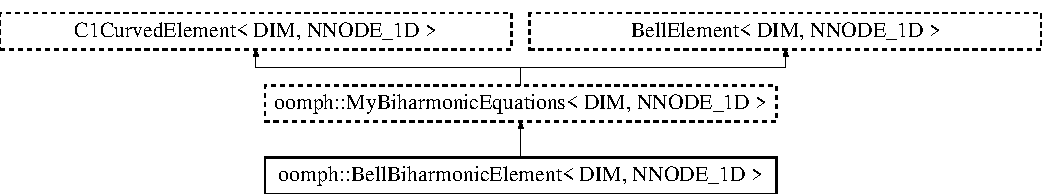
\includegraphics[height=2.608696cm]{classoomph_1_1BellBiharmonicElement}
\end{center}
\end{figure}
\subsection*{Public Member Functions}
\begin{DoxyCompactItemize}
\item 
\hyperlink{classoomph_1_1BellBiharmonicElement_aacb9d267c8aa65057c2c0248b0ef669e}{Bell\+Biharmonic\+Element} ()
\begin{DoxyCompactList}\small\item\em Constructor\+: Call constructors for Bell\+Element and Biharmonic equations. \end{DoxyCompactList}\item 
\hyperlink{classoomph_1_1BellBiharmonicElement_a7fc1038d4814433b0b9e998958309ce5}{Bell\+Biharmonic\+Element} (const \hyperlink{classoomph_1_1BellBiharmonicElement}{Bell\+Biharmonic\+Element}$<$ D\+IM, N\+N\+O\+D\+E\+\_\+1D $>$ \&dummy)
\begin{DoxyCompactList}\small\item\em Broken copy constructor. \end{DoxyCompactList}\item 
unsigned \hyperlink{classoomph_1_1BellBiharmonicElement_a342b59354c4d109da9cda12aad79f293}{required\+\_\+nvalue} (const unsigned \&n) const
\begin{DoxyCompactList}\small\item\em Required \# of `values\textquotesingle{} (pinned or dofs) at node n. \end{DoxyCompactList}\item 
void \hyperlink{classoomph_1_1BellBiharmonicElement_a857d5d7ebdd9eef2b14ef3548fe60e8f}{output} (std\+::ostream \&outfile)
\begin{DoxyCompactList}\small\item\em Output function\+: x,y,u or x,y,z,u. \end{DoxyCompactList}\item 
void \hyperlink{classoomph_1_1BellBiharmonicElement_a558bc65d41a06e864e62eba4d3aa4fa5}{output} (std\+::ostream \&outfile, const unsigned \&n\+\_\+plot)
\begin{DoxyCompactList}\small\item\em Output function\+: x,y,u or x,y,z,u at n\+\_\+plot$^\wedge$\+D\+IM plot points. \end{DoxyCompactList}\item 
void \hyperlink{classoomph_1_1BellBiharmonicElement_a438ad259cc2614b7987542126d92d015}{output} (F\+I\+LE $\ast$file\+\_\+pt)
\begin{DoxyCompactList}\small\item\em C-\/style output function\+: x,y,u or x,y,z,u. \end{DoxyCompactList}\item 
void \hyperlink{classoomph_1_1BellBiharmonicElement_a2c1ef4d6456d860a357dff65fa310bf2}{output} (F\+I\+LE $\ast$file\+\_\+pt, const unsigned \&n\+\_\+plot)
\begin{DoxyCompactList}\small\item\em C-\/style output function\+: x,y,u or x,y,z,u at n\+\_\+plot$^\wedge$\+D\+IM plot points. \end{DoxyCompactList}\item 
void \hyperlink{classoomph_1_1BellBiharmonicElement_a99fcec7056c18d59f747180bd49ef744}{output\+\_\+fct} (std\+::ostream \&outfile, const unsigned \&n\+\_\+plot, Finite\+Element\+::\+Steady\+Exact\+Solution\+Fct\+Pt exact\+\_\+soln\+\_\+pt)
\begin{DoxyCompactList}\small\item\em Output function for an exact solution\+: x,y,u\+\_\+exact or x,y,z,u\+\_\+exact at n\+\_\+plot$^\wedge$\+D\+IM plot points. \end{DoxyCompactList}\item 
void \hyperlink{classoomph_1_1BellBiharmonicElement_a35c7af5c86baeb3787eaf87e2401ea6c}{output\+\_\+fct} (std\+::ostream \&outfile, const unsigned \&n\+\_\+plot, const double \&time, Finite\+Element\+::\+Unsteady\+Exact\+Solution\+Fct\+Pt exact\+\_\+soln\+\_\+pt)
\begin{DoxyCompactList}\small\item\em Output function for a time-\/dependent exact solution. x,y,u\+\_\+exact or x,y,z,u\+\_\+exact at n\+\_\+plot$^\wedge$\+D\+IM plot points (Calls the steady version) \end{DoxyCompactList}\end{DoxyCompactItemize}
\subsection*{Protected Member Functions}
\begin{DoxyCompactItemize}
\item 
double \hyperlink{classoomph_1_1BellBiharmonicElement_af26cb1e9c4980ae4b0911238820f6ae1}{d2shape\+\_\+and\+\_\+d2test\+\_\+eulerian\+\_\+biharmonic} (const Vector$<$ double $>$ \&s, Shape \&psi, D\+Shape \&dpsidx, D\+Shape \&d2psidx, Shape \&test, D\+Shape \&dtestdx, D\+Shape \&d2testdx) const
\begin{DoxyCompactList}\small\item\em Shape, test functions \& derivs. w.\+r.\+t. to global coords. Return Jacobian. \end{DoxyCompactList}\item 
double \hyperlink{classoomph_1_1BellBiharmonicElement_aaa8959c7456a75c15db4b42a70812304}{dshape\+\_\+and\+\_\+dtest\+\_\+eulerian\+\_\+biharmonic} (const Vector$<$ double $>$ \&s, Shape \&psi, D\+Shape \&dpsidx, Shape \&test, D\+Shape \&dtestdx) const
\item 
double \hyperlink{classoomph_1_1BellBiharmonicElement_aceea1798272378f0402ef0e0f324ff3b}{d2shape\+\_\+and\+\_\+d2test\+\_\+eulerian\+\_\+at\+\_\+knot\+\_\+biharmonic} (const unsigned \&ipt, Shape \&psi, D\+Shape \&dpsidx, D\+Shape \&d2psidx, Shape \&test, D\+Shape \&dtestdx, D\+Shape \&d2testdx) const
\begin{DoxyCompactList}\small\item\em Shape, test functions \& derivs. w.\+r.\+t. to global coords. at integration point ipt. Return Jacobian. \end{DoxyCompactList}\item 
double \hyperlink{classoomph_1_1BellBiharmonicElement_ac2875860aa48405076c296341fd778df}{dshape\+\_\+and\+\_\+dtest\+\_\+eulerian\+\_\+at\+\_\+knot\+\_\+biharmonic} (const unsigned \&ipt, Shape \&psi, D\+Shape \&dpsidx, Shape \&test, D\+Shape \&dtestdx) const
\end{DoxyCompactItemize}
\subsection*{Static Private Attributes}
\begin{DoxyCompactItemize}
\item 
static const unsigned \hyperlink{classoomph_1_1BellBiharmonicElement_af13af063a582a21866c4096ef99e67de}{Initial\+\_\+\+Nvalue} = 6
\begin{DoxyCompactList}\small\item\em Static int that holds the number of variables at nodes\+: always the same. \end{DoxyCompactList}\end{DoxyCompactItemize}
\subsection*{Additional Inherited Members}


\subsection{Detailed Description}
\subsubsection*{template$<$unsigned D\+IM, unsigned N\+N\+O\+D\+E\+\_\+1D$>$\newline
class oomph\+::\+Bell\+Biharmonic\+Element$<$ D\+I\+M, N\+N\+O\+D\+E\+\_\+1\+D $>$}

\hyperlink{classoomph_1_1BellBiharmonicElement}{Bell\+Biharmonic\+Element} elements are a subparametric scheme with linear Lagrange interpolation for approximating the geometry and the C1-\/functions for approximating variables. 

Definition at line 311 of file unstructured\+\_\+2d\+\_\+biharmonic\+\_\+bellelement.\+cc.



\subsection{Constructor \& Destructor Documentation}
\mbox{\Hypertarget{classoomph_1_1BellBiharmonicElement_aacb9d267c8aa65057c2c0248b0ef669e}\label{classoomph_1_1BellBiharmonicElement_aacb9d267c8aa65057c2c0248b0ef669e}} 
\index{oomph\+::\+Bell\+Biharmonic\+Element@{oomph\+::\+Bell\+Biharmonic\+Element}!Bell\+Biharmonic\+Element@{Bell\+Biharmonic\+Element}}
\index{Bell\+Biharmonic\+Element@{Bell\+Biharmonic\+Element}!oomph\+::\+Bell\+Biharmonic\+Element@{oomph\+::\+Bell\+Biharmonic\+Element}}
\subsubsection{\texorpdfstring{Bell\+Biharmonic\+Element()}{BellBiharmonicElement()}\hspace{0.1cm}{\footnotesize\ttfamily [1/2]}}
{\footnotesize\ttfamily template$<$unsigned D\+IM, unsigned N\+N\+O\+D\+E\+\_\+1D$>$ \\
\hyperlink{classoomph_1_1BellBiharmonicElement}{oomph\+::\+Bell\+Biharmonic\+Element}$<$ D\+IM, N\+N\+O\+D\+E\+\_\+1D $>$\+::\hyperlink{classoomph_1_1BellBiharmonicElement}{Bell\+Biharmonic\+Element} (\begin{DoxyParamCaption}{ }\end{DoxyParamCaption})\hspace{0.3cm}{\ttfamily [inline]}}



Constructor\+: Call constructors for Bell\+Element and Biharmonic equations. 



Definition at line 325 of file unstructured\+\_\+2d\+\_\+biharmonic\+\_\+bellelement.\+cc.

\mbox{\Hypertarget{classoomph_1_1BellBiharmonicElement_a7fc1038d4814433b0b9e998958309ce5}\label{classoomph_1_1BellBiharmonicElement_a7fc1038d4814433b0b9e998958309ce5}} 
\index{oomph\+::\+Bell\+Biharmonic\+Element@{oomph\+::\+Bell\+Biharmonic\+Element}!Bell\+Biharmonic\+Element@{Bell\+Biharmonic\+Element}}
\index{Bell\+Biharmonic\+Element@{Bell\+Biharmonic\+Element}!oomph\+::\+Bell\+Biharmonic\+Element@{oomph\+::\+Bell\+Biharmonic\+Element}}
\subsubsection{\texorpdfstring{Bell\+Biharmonic\+Element()}{BellBiharmonicElement()}\hspace{0.1cm}{\footnotesize\ttfamily [2/2]}}
{\footnotesize\ttfamily template$<$unsigned D\+IM, unsigned N\+N\+O\+D\+E\+\_\+1D$>$ \\
\hyperlink{classoomph_1_1BellBiharmonicElement}{oomph\+::\+Bell\+Biharmonic\+Element}$<$ D\+IM, N\+N\+O\+D\+E\+\_\+1D $>$\+::\hyperlink{classoomph_1_1BellBiharmonicElement}{Bell\+Biharmonic\+Element} (\begin{DoxyParamCaption}\item[{const \hyperlink{classoomph_1_1BellBiharmonicElement}{Bell\+Biharmonic\+Element}$<$ D\+IM, N\+N\+O\+D\+E\+\_\+1D $>$ \&}]{dummy }\end{DoxyParamCaption})\hspace{0.3cm}{\ttfamily [inline]}}



Broken copy constructor. 



Definition at line 329 of file unstructured\+\_\+2d\+\_\+biharmonic\+\_\+bellelement.\+cc.



\subsection{Member Function Documentation}
\mbox{\Hypertarget{classoomph_1_1BellBiharmonicElement_aceea1798272378f0402ef0e0f324ff3b}\label{classoomph_1_1BellBiharmonicElement_aceea1798272378f0402ef0e0f324ff3b}} 
\index{oomph\+::\+Bell\+Biharmonic\+Element@{oomph\+::\+Bell\+Biharmonic\+Element}!d2shape\+\_\+and\+\_\+d2test\+\_\+eulerian\+\_\+at\+\_\+knot\+\_\+biharmonic@{d2shape\+\_\+and\+\_\+d2test\+\_\+eulerian\+\_\+at\+\_\+knot\+\_\+biharmonic}}
\index{d2shape\+\_\+and\+\_\+d2test\+\_\+eulerian\+\_\+at\+\_\+knot\+\_\+biharmonic@{d2shape\+\_\+and\+\_\+d2test\+\_\+eulerian\+\_\+at\+\_\+knot\+\_\+biharmonic}!oomph\+::\+Bell\+Biharmonic\+Element@{oomph\+::\+Bell\+Biharmonic\+Element}}
\subsubsection{\texorpdfstring{d2shape\+\_\+and\+\_\+d2test\+\_\+eulerian\+\_\+at\+\_\+knot\+\_\+biharmonic()}{d2shape\_and\_d2test\_eulerian\_at\_knot\_biharmonic()}}
{\footnotesize\ttfamily template$<$unsigned D\+IM, unsigned N\+N\+O\+D\+E\+\_\+1D$>$ \\
double \hyperlink{classoomph_1_1BellBiharmonicElement}{oomph\+::\+Bell\+Biharmonic\+Element}$<$ D\+IM, N\+N\+O\+D\+E\+\_\+1D $>$\+::d2shape\+\_\+and\+\_\+d2test\+\_\+eulerian\+\_\+at\+\_\+knot\+\_\+biharmonic (\begin{DoxyParamCaption}\item[{const unsigned \&}]{ipt,  }\item[{Shape \&}]{psi,  }\item[{D\+Shape \&}]{dpsidx,  }\item[{D\+Shape \&}]{d2psidx,  }\item[{Shape \&}]{test,  }\item[{D\+Shape \&}]{dtestdx,  }\item[{D\+Shape \&}]{d2testdx }\end{DoxyParamCaption}) const\hspace{0.3cm}{\ttfamily [inline]}, {\ttfamily [protected]}, {\ttfamily [virtual]}}



Shape, test functions \& derivs. w.\+r.\+t. to global coords. at integration point ipt. Return Jacobian. 



Implements \hyperlink{classoomph_1_1MyBiharmonicEquations_a85687f39c0fb72f25ce67f5867a83470}{oomph\+::\+My\+Biharmonic\+Equations$<$ D\+I\+M, N\+N\+O\+D\+E\+\_\+1\+D $>$}.



Definition at line 517 of file unstructured\+\_\+2d\+\_\+biharmonic\+\_\+bellelement.\+cc.

\mbox{\Hypertarget{classoomph_1_1BellBiharmonicElement_af26cb1e9c4980ae4b0911238820f6ae1}\label{classoomph_1_1BellBiharmonicElement_af26cb1e9c4980ae4b0911238820f6ae1}} 
\index{oomph\+::\+Bell\+Biharmonic\+Element@{oomph\+::\+Bell\+Biharmonic\+Element}!d2shape\+\_\+and\+\_\+d2test\+\_\+eulerian\+\_\+biharmonic@{d2shape\+\_\+and\+\_\+d2test\+\_\+eulerian\+\_\+biharmonic}}
\index{d2shape\+\_\+and\+\_\+d2test\+\_\+eulerian\+\_\+biharmonic@{d2shape\+\_\+and\+\_\+d2test\+\_\+eulerian\+\_\+biharmonic}!oomph\+::\+Bell\+Biharmonic\+Element@{oomph\+::\+Bell\+Biharmonic\+Element}}
\subsubsection{\texorpdfstring{d2shape\+\_\+and\+\_\+d2test\+\_\+eulerian\+\_\+biharmonic()}{d2shape\_and\_d2test\_eulerian\_biharmonic()}}
{\footnotesize\ttfamily template$<$unsigned D\+IM, unsigned N\+N\+O\+D\+E\+\_\+1D$>$ \\
double \hyperlink{classoomph_1_1BellBiharmonicElement}{oomph\+::\+Bell\+Biharmonic\+Element}$<$ D\+IM, N\+N\+O\+D\+E\+\_\+1D $>$\+::d2shape\+\_\+and\+\_\+d2test\+\_\+eulerian\+\_\+biharmonic (\begin{DoxyParamCaption}\item[{const Vector$<$ double $>$ \&}]{s,  }\item[{Shape \&}]{psi,  }\item[{D\+Shape \&}]{dpsidx,  }\item[{D\+Shape \&}]{d2psidx,  }\item[{Shape \&}]{test,  }\item[{D\+Shape \&}]{dtestdx,  }\item[{D\+Shape \&}]{d2testdx }\end{DoxyParamCaption}) const\hspace{0.3cm}{\ttfamily [inline]}, {\ttfamily [protected]}, {\ttfamily [virtual]}}



Shape, test functions \& derivs. w.\+r.\+t. to global coords. Return Jacobian. 



Implements \hyperlink{classoomph_1_1MyBiharmonicEquations_a4597b3938b6f1244d6e8e0f58250c14a}{oomph\+::\+My\+Biharmonic\+Equations$<$ D\+I\+M, N\+N\+O\+D\+E\+\_\+1\+D $>$}.



Definition at line 471 of file unstructured\+\_\+2d\+\_\+biharmonic\+\_\+bellelement.\+cc.

\mbox{\Hypertarget{classoomph_1_1BellBiharmonicElement_ac2875860aa48405076c296341fd778df}\label{classoomph_1_1BellBiharmonicElement_ac2875860aa48405076c296341fd778df}} 
\index{oomph\+::\+Bell\+Biharmonic\+Element@{oomph\+::\+Bell\+Biharmonic\+Element}!dshape\+\_\+and\+\_\+dtest\+\_\+eulerian\+\_\+at\+\_\+knot\+\_\+biharmonic@{dshape\+\_\+and\+\_\+dtest\+\_\+eulerian\+\_\+at\+\_\+knot\+\_\+biharmonic}}
\index{dshape\+\_\+and\+\_\+dtest\+\_\+eulerian\+\_\+at\+\_\+knot\+\_\+biharmonic@{dshape\+\_\+and\+\_\+dtest\+\_\+eulerian\+\_\+at\+\_\+knot\+\_\+biharmonic}!oomph\+::\+Bell\+Biharmonic\+Element@{oomph\+::\+Bell\+Biharmonic\+Element}}
\subsubsection{\texorpdfstring{dshape\+\_\+and\+\_\+dtest\+\_\+eulerian\+\_\+at\+\_\+knot\+\_\+biharmonic()}{dshape\_and\_dtest\_eulerian\_at\_knot\_biharmonic()}}
{\footnotesize\ttfamily template$<$unsigned D\+IM, unsigned N\+N\+O\+D\+E\+\_\+1D$>$ \\
double \hyperlink{classoomph_1_1BellBiharmonicElement}{oomph\+::\+Bell\+Biharmonic\+Element}$<$ D\+IM, N\+N\+O\+D\+E\+\_\+1D $>$\+::dshape\+\_\+and\+\_\+dtest\+\_\+eulerian\+\_\+at\+\_\+knot\+\_\+biharmonic (\begin{DoxyParamCaption}\item[{const unsigned \&}]{ipt,  }\item[{Shape \&}]{psi,  }\item[{D\+Shape \&}]{dpsidx,  }\item[{Shape \&}]{test,  }\item[{D\+Shape \&}]{dtestdx }\end{DoxyParamCaption}) const\hspace{0.3cm}{\ttfamily [inline]}, {\ttfamily [protected]}, {\ttfamily [virtual]}}

Define the shape functions and test functions and derivatives w.\+r.\+t. global coordinates and return Jacobian of mapping.

Galerkin\+: Test functions = shape functions 

Implements \hyperlink{classoomph_1_1MyBiharmonicEquations_a08e45fddb2c25119e6ba826cd6cafdbf}{oomph\+::\+My\+Biharmonic\+Equations$<$ D\+I\+M, N\+N\+O\+D\+E\+\_\+1\+D $>$}.



Definition at line 503 of file unstructured\+\_\+2d\+\_\+biharmonic\+\_\+bellelement.\+cc.

\mbox{\Hypertarget{classoomph_1_1BellBiharmonicElement_aaa8959c7456a75c15db4b42a70812304}\label{classoomph_1_1BellBiharmonicElement_aaa8959c7456a75c15db4b42a70812304}} 
\index{oomph\+::\+Bell\+Biharmonic\+Element@{oomph\+::\+Bell\+Biharmonic\+Element}!dshape\+\_\+and\+\_\+dtest\+\_\+eulerian\+\_\+biharmonic@{dshape\+\_\+and\+\_\+dtest\+\_\+eulerian\+\_\+biharmonic}}
\index{dshape\+\_\+and\+\_\+dtest\+\_\+eulerian\+\_\+biharmonic@{dshape\+\_\+and\+\_\+dtest\+\_\+eulerian\+\_\+biharmonic}!oomph\+::\+Bell\+Biharmonic\+Element@{oomph\+::\+Bell\+Biharmonic\+Element}}
\subsubsection{\texorpdfstring{dshape\+\_\+and\+\_\+dtest\+\_\+eulerian\+\_\+biharmonic()}{dshape\_and\_dtest\_eulerian\_biharmonic()}}
{\footnotesize\ttfamily template$<$unsigned D\+IM, unsigned N\+N\+O\+D\+E\+\_\+1D$>$ \\
double \hyperlink{classoomph_1_1BellBiharmonicElement}{oomph\+::\+Bell\+Biharmonic\+Element}$<$ D\+IM, N\+N\+O\+D\+E\+\_\+1D $>$\+::dshape\+\_\+and\+\_\+dtest\+\_\+eulerian\+\_\+biharmonic (\begin{DoxyParamCaption}\item[{const Vector$<$ double $>$ \&}]{s,  }\item[{Shape \&}]{psi,  }\item[{D\+Shape \&}]{dpsidx,  }\item[{Shape \&}]{test,  }\item[{D\+Shape \&}]{dtestdx }\end{DoxyParamCaption}) const\hspace{0.3cm}{\ttfamily [inline]}, {\ttfamily [protected]}, {\ttfamily [virtual]}}

Define the shape functions and test functions and derivatives w.\+r.\+t. global coordinates and return Jacobian of mapping.

Galerkin\+: Test functions = shape functions 

Implements \hyperlink{classoomph_1_1MyBiharmonicEquations_a084eaadd62185dad622c7708862f023a}{oomph\+::\+My\+Biharmonic\+Equations$<$ D\+I\+M, N\+N\+O\+D\+E\+\_\+1\+D $>$}.



Definition at line 455 of file unstructured\+\_\+2d\+\_\+biharmonic\+\_\+bellelement.\+cc.

\mbox{\Hypertarget{classoomph_1_1BellBiharmonicElement_a857d5d7ebdd9eef2b14ef3548fe60e8f}\label{classoomph_1_1BellBiharmonicElement_a857d5d7ebdd9eef2b14ef3548fe60e8f}} 
\index{oomph\+::\+Bell\+Biharmonic\+Element@{oomph\+::\+Bell\+Biharmonic\+Element}!output@{output}}
\index{output@{output}!oomph\+::\+Bell\+Biharmonic\+Element@{oomph\+::\+Bell\+Biharmonic\+Element}}
\subsubsection{\texorpdfstring{output()}{output()}\hspace{0.1cm}{\footnotesize\ttfamily [1/4]}}
{\footnotesize\ttfamily template$<$unsigned D\+IM, unsigned N\+N\+O\+D\+E\+\_\+1D$>$ \\
void \hyperlink{classoomph_1_1BellBiharmonicElement}{oomph\+::\+Bell\+Biharmonic\+Element}$<$ D\+IM, N\+N\+O\+D\+E\+\_\+1D $>$\+::output (\begin{DoxyParamCaption}\item[{std\+::ostream \&}]{outfile }\end{DoxyParamCaption})\hspace{0.3cm}{\ttfamily [inline]}}



Output function\+: x,y,u or x,y,z,u. 



Definition at line 342 of file unstructured\+\_\+2d\+\_\+biharmonic\+\_\+bellelement.\+cc.

\mbox{\Hypertarget{classoomph_1_1BellBiharmonicElement_a558bc65d41a06e864e62eba4d3aa4fa5}\label{classoomph_1_1BellBiharmonicElement_a558bc65d41a06e864e62eba4d3aa4fa5}} 
\index{oomph\+::\+Bell\+Biharmonic\+Element@{oomph\+::\+Bell\+Biharmonic\+Element}!output@{output}}
\index{output@{output}!oomph\+::\+Bell\+Biharmonic\+Element@{oomph\+::\+Bell\+Biharmonic\+Element}}
\subsubsection{\texorpdfstring{output()}{output()}\hspace{0.1cm}{\footnotesize\ttfamily [2/4]}}
{\footnotesize\ttfamily template$<$unsigned D\+IM, unsigned N\+N\+O\+D\+E\+\_\+1D$>$ \\
void \hyperlink{classoomph_1_1BellBiharmonicElement}{oomph\+::\+Bell\+Biharmonic\+Element}$<$ D\+IM, N\+N\+O\+D\+E\+\_\+1D $>$\+::output (\begin{DoxyParamCaption}\item[{std\+::ostream \&}]{outfile,  }\item[{const unsigned \&}]{n\+\_\+plot }\end{DoxyParamCaption})\hspace{0.3cm}{\ttfamily [inline]}}



Output function\+: x,y,u or x,y,z,u at n\+\_\+plot$^\wedge$\+D\+IM plot points. 



Definition at line 348 of file unstructured\+\_\+2d\+\_\+biharmonic\+\_\+bellelement.\+cc.

\mbox{\Hypertarget{classoomph_1_1BellBiharmonicElement_a438ad259cc2614b7987542126d92d015}\label{classoomph_1_1BellBiharmonicElement_a438ad259cc2614b7987542126d92d015}} 
\index{oomph\+::\+Bell\+Biharmonic\+Element@{oomph\+::\+Bell\+Biharmonic\+Element}!output@{output}}
\index{output@{output}!oomph\+::\+Bell\+Biharmonic\+Element@{oomph\+::\+Bell\+Biharmonic\+Element}}
\subsubsection{\texorpdfstring{output()}{output()}\hspace{0.1cm}{\footnotesize\ttfamily [3/4]}}
{\footnotesize\ttfamily template$<$unsigned D\+IM, unsigned N\+N\+O\+D\+E\+\_\+1D$>$ \\
void \hyperlink{classoomph_1_1BellBiharmonicElement}{oomph\+::\+Bell\+Biharmonic\+Element}$<$ D\+IM, N\+N\+O\+D\+E\+\_\+1D $>$\+::output (\begin{DoxyParamCaption}\item[{F\+I\+LE $\ast$}]{file\+\_\+pt }\end{DoxyParamCaption})\hspace{0.3cm}{\ttfamily [inline]}}



C-\/style output function\+: x,y,u or x,y,z,u. 



Definition at line 354 of file unstructured\+\_\+2d\+\_\+biharmonic\+\_\+bellelement.\+cc.

\mbox{\Hypertarget{classoomph_1_1BellBiharmonicElement_a2c1ef4d6456d860a357dff65fa310bf2}\label{classoomph_1_1BellBiharmonicElement_a2c1ef4d6456d860a357dff65fa310bf2}} 
\index{oomph\+::\+Bell\+Biharmonic\+Element@{oomph\+::\+Bell\+Biharmonic\+Element}!output@{output}}
\index{output@{output}!oomph\+::\+Bell\+Biharmonic\+Element@{oomph\+::\+Bell\+Biharmonic\+Element}}
\subsubsection{\texorpdfstring{output()}{output()}\hspace{0.1cm}{\footnotesize\ttfamily [4/4]}}
{\footnotesize\ttfamily template$<$unsigned D\+IM, unsigned N\+N\+O\+D\+E\+\_\+1D$>$ \\
void \hyperlink{classoomph_1_1BellBiharmonicElement}{oomph\+::\+Bell\+Biharmonic\+Element}$<$ D\+IM, N\+N\+O\+D\+E\+\_\+1D $>$\+::output (\begin{DoxyParamCaption}\item[{F\+I\+LE $\ast$}]{file\+\_\+pt,  }\item[{const unsigned \&}]{n\+\_\+plot }\end{DoxyParamCaption})\hspace{0.3cm}{\ttfamily [inline]}}



C-\/style output function\+: x,y,u or x,y,z,u at n\+\_\+plot$^\wedge$\+D\+IM plot points. 



Definition at line 360 of file unstructured\+\_\+2d\+\_\+biharmonic\+\_\+bellelement.\+cc.

\mbox{\Hypertarget{classoomph_1_1BellBiharmonicElement_a99fcec7056c18d59f747180bd49ef744}\label{classoomph_1_1BellBiharmonicElement_a99fcec7056c18d59f747180bd49ef744}} 
\index{oomph\+::\+Bell\+Biharmonic\+Element@{oomph\+::\+Bell\+Biharmonic\+Element}!output\+\_\+fct@{output\+\_\+fct}}
\index{output\+\_\+fct@{output\+\_\+fct}!oomph\+::\+Bell\+Biharmonic\+Element@{oomph\+::\+Bell\+Biharmonic\+Element}}
\subsubsection{\texorpdfstring{output\+\_\+fct()}{output\_fct()}\hspace{0.1cm}{\footnotesize\ttfamily [1/2]}}
{\footnotesize\ttfamily template$<$unsigned D\+IM, unsigned N\+N\+O\+D\+E\+\_\+1D$>$ \\
void \hyperlink{classoomph_1_1BellBiharmonicElement}{oomph\+::\+Bell\+Biharmonic\+Element}$<$ D\+IM, N\+N\+O\+D\+E\+\_\+1D $>$\+::output\+\_\+fct (\begin{DoxyParamCaption}\item[{std\+::ostream \&}]{outfile,  }\item[{const unsigned \&}]{n\+\_\+plot,  }\item[{Finite\+Element\+::\+Steady\+Exact\+Solution\+Fct\+Pt}]{exact\+\_\+soln\+\_\+pt }\end{DoxyParamCaption})\hspace{0.3cm}{\ttfamily [inline]}}



Output function for an exact solution\+: x,y,u\+\_\+exact or x,y,z,u\+\_\+exact at n\+\_\+plot$^\wedge$\+D\+IM plot points. 



Definition at line 366 of file unstructured\+\_\+2d\+\_\+biharmonic\+\_\+bellelement.\+cc.

\mbox{\Hypertarget{classoomph_1_1BellBiharmonicElement_a35c7af5c86baeb3787eaf87e2401ea6c}\label{classoomph_1_1BellBiharmonicElement_a35c7af5c86baeb3787eaf87e2401ea6c}} 
\index{oomph\+::\+Bell\+Biharmonic\+Element@{oomph\+::\+Bell\+Biharmonic\+Element}!output\+\_\+fct@{output\+\_\+fct}}
\index{output\+\_\+fct@{output\+\_\+fct}!oomph\+::\+Bell\+Biharmonic\+Element@{oomph\+::\+Bell\+Biharmonic\+Element}}
\subsubsection{\texorpdfstring{output\+\_\+fct()}{output\_fct()}\hspace{0.1cm}{\footnotesize\ttfamily [2/2]}}
{\footnotesize\ttfamily template$<$unsigned D\+IM, unsigned N\+N\+O\+D\+E\+\_\+1D$>$ \\
void \hyperlink{classoomph_1_1BellBiharmonicElement}{oomph\+::\+Bell\+Biharmonic\+Element}$<$ D\+IM, N\+N\+O\+D\+E\+\_\+1D $>$\+::output\+\_\+fct (\begin{DoxyParamCaption}\item[{std\+::ostream \&}]{outfile,  }\item[{const unsigned \&}]{n\+\_\+plot,  }\item[{const double \&}]{time,  }\item[{Finite\+Element\+::\+Unsteady\+Exact\+Solution\+Fct\+Pt}]{exact\+\_\+soln\+\_\+pt }\end{DoxyParamCaption})\hspace{0.3cm}{\ttfamily [inline]}, {\ttfamily [virtual]}}



Output function for a time-\/dependent exact solution. x,y,u\+\_\+exact or x,y,z,u\+\_\+exact at n\+\_\+plot$^\wedge$\+D\+IM plot points (Calls the steady version) 



Reimplemented from \hyperlink{classoomph_1_1MyBiharmonicEquations_a95b35b18fac5212ade1a81c26657bcdb}{oomph\+::\+My\+Biharmonic\+Equations$<$ D\+I\+M, N\+N\+O\+D\+E\+\_\+1\+D $>$}.



Definition at line 375 of file unstructured\+\_\+2d\+\_\+biharmonic\+\_\+bellelement.\+cc.

\mbox{\Hypertarget{classoomph_1_1BellBiharmonicElement_a342b59354c4d109da9cda12aad79f293}\label{classoomph_1_1BellBiharmonicElement_a342b59354c4d109da9cda12aad79f293}} 
\index{oomph\+::\+Bell\+Biharmonic\+Element@{oomph\+::\+Bell\+Biharmonic\+Element}!required\+\_\+nvalue@{required\+\_\+nvalue}}
\index{required\+\_\+nvalue@{required\+\_\+nvalue}!oomph\+::\+Bell\+Biharmonic\+Element@{oomph\+::\+Bell\+Biharmonic\+Element}}
\subsubsection{\texorpdfstring{required\+\_\+nvalue()}{required\_nvalue()}}
{\footnotesize\ttfamily template$<$unsigned D\+IM, unsigned N\+N\+O\+D\+E\+\_\+1D$>$ \\
unsigned \hyperlink{classoomph_1_1BellBiharmonicElement}{oomph\+::\+Bell\+Biharmonic\+Element}$<$ D\+IM, N\+N\+O\+D\+E\+\_\+1D $>$\+::required\+\_\+nvalue (\begin{DoxyParamCaption}\item[{const unsigned \&}]{n }\end{DoxyParamCaption}) const\hspace{0.3cm}{\ttfamily [inline]}}



Required \# of `values\textquotesingle{} (pinned or dofs) at node n. 



Definition at line 337 of file unstructured\+\_\+2d\+\_\+biharmonic\+\_\+bellelement.\+cc.



\subsection{Member Data Documentation}
\mbox{\Hypertarget{classoomph_1_1BellBiharmonicElement_af13af063a582a21866c4096ef99e67de}\label{classoomph_1_1BellBiharmonicElement_af13af063a582a21866c4096ef99e67de}} 
\index{oomph\+::\+Bell\+Biharmonic\+Element@{oomph\+::\+Bell\+Biharmonic\+Element}!Initial\+\_\+\+Nvalue@{Initial\+\_\+\+Nvalue}}
\index{Initial\+\_\+\+Nvalue@{Initial\+\_\+\+Nvalue}!oomph\+::\+Bell\+Biharmonic\+Element@{oomph\+::\+Bell\+Biharmonic\+Element}}
\subsubsection{\texorpdfstring{Initial\+\_\+\+Nvalue}{Initial\_Nvalue}}
{\footnotesize\ttfamily template$<$unsigned D\+IM, unsigned N\+N\+O\+D\+E\+\_\+1D$>$ \\
const unsigned \hyperlink{classoomph_1_1BellBiharmonicElement}{oomph\+::\+Bell\+Biharmonic\+Element}$<$ D\+IM, N\+N\+O\+D\+E\+\_\+1D $>$\+::Initial\+\_\+\+Nvalue = 6\hspace{0.3cm}{\ttfamily [static]}, {\ttfamily [private]}}



Static int that holds the number of variables at nodes\+: always the same. 

Set the data for the number of Variables at each node. 

Definition at line 318 of file unstructured\+\_\+2d\+\_\+biharmonic\+\_\+bellelement.\+cc.



The documentation for this class was generated from the following file\+:\begin{DoxyCompactItemize}
\item 
\hyperlink{unstructured__2d__biharmonic__bellelement_8cc}{unstructured\+\_\+2d\+\_\+biharmonic\+\_\+bellelement.\+cc}\end{DoxyCompactItemize}

\hypertarget{classoomph_1_1BiharmonicCurvedElement}{}\section{oomph\+:\+:Biharmonic\+Curved\+Element$<$ D\+IM, N\+N\+O\+D\+E\+\_\+1D $>$ Class Template Reference}
\label{classoomph_1_1BiharmonicCurvedElement}\index{oomph\+::\+Biharmonic\+Curved\+Element$<$ D\+I\+M, N\+N\+O\+D\+E\+\_\+1\+D $>$@{oomph\+::\+Biharmonic\+Curved\+Element$<$ D\+I\+M, N\+N\+O\+D\+E\+\_\+1\+D $>$}}
Inheritance diagram for oomph\+:\+:Biharmonic\+Curved\+Element$<$ D\+IM, N\+N\+O\+D\+E\+\_\+1D $>$\+:\begin{figure}[H]
\begin{center}
\leavevmode
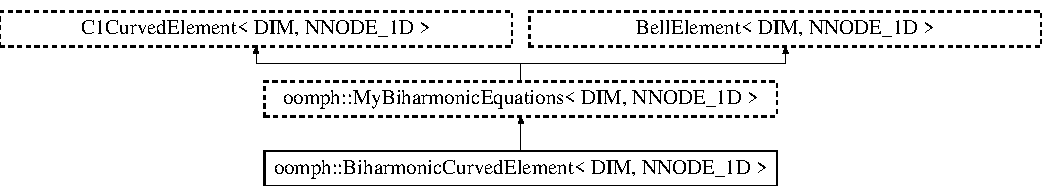
\includegraphics[height=2.500000cm]{classoomph_1_1BiharmonicCurvedElement}
\end{center}
\end{figure}
\subsection*{Public Member Functions}
\begin{DoxyCompactItemize}
\item 
\hyperlink{classoomph_1_1BiharmonicCurvedElement_a29bf3b21c60da246d8bc9abfd0e91bf5}{Biharmonic\+Curved\+Element} ()
\begin{DoxyCompactList}\small\item\em Constructor\+: Call constructors for C1\+Curved\+Element and Biharmonic equations. \end{DoxyCompactList}\item 
\hyperlink{classoomph_1_1BiharmonicCurvedElement_a20723b0ce340d7ddb7823f83c3d504ee}{Biharmonic\+Curved\+Element} (const \hyperlink{classoomph_1_1BiharmonicCurvedElement}{Biharmonic\+Curved\+Element}$<$ D\+IM, N\+N\+O\+D\+E\+\_\+1D $>$ \&dummy)
\begin{DoxyCompactList}\small\item\em Broken copy constructor. \end{DoxyCompactList}\item 
unsigned \hyperlink{classoomph_1_1BiharmonicCurvedElement_a335d075769ca949eed1d1ab5482a6e46}{required\+\_\+nvalue} (const unsigned \&n) const
\begin{DoxyCompactList}\small\item\em Required \# of `values\textquotesingle{} (pinned or dofs) at node n. \end{DoxyCompactList}\item 
void \hyperlink{classoomph_1_1BiharmonicCurvedElement_a702f7fef5954cb750e30579ce4a8a0da}{output} (std\+::ostream \&outfile)
\begin{DoxyCompactList}\small\item\em Output function\+: x,y,u or x,y,z,u. \end{DoxyCompactList}\item 
void \hyperlink{classoomph_1_1BiharmonicCurvedElement_ac6229a99465efed7ef1852806f12772e}{output} (std\+::ostream \&outfile, const unsigned \&n\+\_\+plot)
\begin{DoxyCompactList}\small\item\em Output function\+: x,y,u or x,y,z,u at n\+\_\+plot$^\wedge$\+D\+IM plot points. \end{DoxyCompactList}\item 
void \hyperlink{classoomph_1_1BiharmonicCurvedElement_a6bb84710cab6c0c27c90e2b0675ff6cd}{output} (F\+I\+LE $\ast$file\+\_\+pt)
\begin{DoxyCompactList}\small\item\em C-\/style output function\+: x,y,u or x,y,z,u. \end{DoxyCompactList}\item 
void \hyperlink{classoomph_1_1BiharmonicCurvedElement_a7a5dfc6d78fcd52385395cca7a125772}{output} (F\+I\+LE $\ast$file\+\_\+pt, const unsigned \&n\+\_\+plot)
\begin{DoxyCompactList}\small\item\em C-\/style output function\+: x,y,u or x,y,z,u at n\+\_\+plot$^\wedge$\+D\+IM plot points. \end{DoxyCompactList}\item 
void \hyperlink{classoomph_1_1BiharmonicCurvedElement_a19906845c3b1678b6d193b46038042c6}{output\+\_\+fct} (std\+::ostream \&outfile, const unsigned \&n\+\_\+plot, Finite\+Element\+::\+Steady\+Exact\+Solution\+Fct\+Pt exact\+\_\+soln\+\_\+pt)
\begin{DoxyCompactList}\small\item\em Output function for an exact solution\+: x,y,u\+\_\+exact or x,y,z,u\+\_\+exact at n\+\_\+plot$^\wedge$\+D\+IM plot points. \end{DoxyCompactList}\item 
void \hyperlink{classoomph_1_1BiharmonicCurvedElement_a50187fb5a3a0a5905590ed7cd6780211}{output\+\_\+fct} (std\+::ostream \&outfile, const unsigned \&n\+\_\+plot, const double \&time, Finite\+Element\+::\+Unsteady\+Exact\+Solution\+Fct\+Pt exact\+\_\+soln\+\_\+pt)
\begin{DoxyCompactList}\small\item\em Output function for a time-\/dependent exact solution. x,y,u\+\_\+exact or x,y,z,u\+\_\+exact at n\+\_\+plot$^\wedge$\+D\+IM plot points (Calls the steady version) \end{DoxyCompactList}\end{DoxyCompactItemize}
\subsection*{Protected Member Functions}
\begin{DoxyCompactItemize}
\item 
double \hyperlink{classoomph_1_1BiharmonicCurvedElement_aabae0edfbfa93f138e7a2c6421dfcfcd}{d2shape\+\_\+and\+\_\+d2test\+\_\+eulerian\+\_\+biharmonic} (const Vector$<$ double $>$ \&s, Shape \&psi, D\+Shape \&dpsidx, D\+Shape \&d2psidx, Shape \&test, D\+Shape \&dtestdx, D\+Shape \&d2testdx) const
\begin{DoxyCompactList}\small\item\em Shape, test functions \& derivs. w.\+r.\+t. to global coords. Return Jacobian. \end{DoxyCompactList}\item 
double \hyperlink{classoomph_1_1BiharmonicCurvedElement_a3dcacc1730a9bf9bf8f7396a795ce6b6}{dshape\+\_\+and\+\_\+dtest\+\_\+eulerian\+\_\+biharmonic} (const Vector$<$ double $>$ \&s, Shape \&psi, D\+Shape \&dpsidx, Shape \&test, D\+Shape \&dtestdx) const
\item 
double \hyperlink{classoomph_1_1BiharmonicCurvedElement_a89720b99d24708f02135502625ad7e3c}{d2shape\+\_\+and\+\_\+d2test\+\_\+eulerian\+\_\+at\+\_\+knot\+\_\+biharmonic} (const unsigned \&ipt, Shape \&psi, D\+Shape \&dpsidx, D\+Shape \&d2psidx, Shape \&test, D\+Shape \&dtestdx, D\+Shape \&d2testdx) const
\begin{DoxyCompactList}\small\item\em Shape, test functions \& derivs. w.\+r.\+t. to global coords. at integration point ipt. Return Jacobian. \end{DoxyCompactList}\item 
double \hyperlink{classoomph_1_1BiharmonicCurvedElement_a41fe37c99757e9da1181e4e769752915}{dshape\+\_\+and\+\_\+dtest\+\_\+eulerian\+\_\+at\+\_\+knot\+\_\+biharmonic} (const unsigned \&ipt, Shape \&psi, D\+Shape \&dpsidx, Shape \&test, D\+Shape \&dtestdx) const
\end{DoxyCompactItemize}
\subsection*{Static Private Attributes}
\begin{DoxyCompactItemize}
\item 
static const unsigned \hyperlink{classoomph_1_1BiharmonicCurvedElement_a67e3e0d226505fa7f24eedab2f9d744c}{Initial\+\_\+\+Nvalue} = 6
\begin{DoxyCompactList}\small\item\em Static int that holds the number of variables at nodes\+: always the same. \end{DoxyCompactList}\end{DoxyCompactItemize}
\subsection*{Additional Inherited Members}


\subsection{Detailed Description}
\subsubsection*{template$<$unsigned D\+IM, unsigned N\+N\+O\+D\+E\+\_\+1D$>$\newline
class oomph\+::\+Biharmonic\+Curved\+Element$<$ D\+I\+M, N\+N\+O\+D\+E\+\_\+1\+D $>$}

\hyperlink{classoomph_1_1BiharmonicCurvedElement}{Biharmonic\+Curved\+Element} elements are a subparametric scheme with a Lagrange interpolation for approximating the geometry and the C1-\/functions for approximating variables. 

Definition at line 332 of file unstructured\+\_\+2d\+\_\+biharmonic\+\_\+curvedelement.\+cc.



\subsection{Constructor \& Destructor Documentation}
\mbox{\Hypertarget{classoomph_1_1BiharmonicCurvedElement_a29bf3b21c60da246d8bc9abfd0e91bf5}\label{classoomph_1_1BiharmonicCurvedElement_a29bf3b21c60da246d8bc9abfd0e91bf5}} 
\index{oomph\+::\+Biharmonic\+Curved\+Element@{oomph\+::\+Biharmonic\+Curved\+Element}!Biharmonic\+Curved\+Element@{Biharmonic\+Curved\+Element}}
\index{Biharmonic\+Curved\+Element@{Biharmonic\+Curved\+Element}!oomph\+::\+Biharmonic\+Curved\+Element@{oomph\+::\+Biharmonic\+Curved\+Element}}
\subsubsection{\texorpdfstring{Biharmonic\+Curved\+Element()}{BiharmonicCurvedElement()}\hspace{0.1cm}{\footnotesize\ttfamily [1/2]}}
{\footnotesize\ttfamily template$<$unsigned D\+IM, unsigned N\+N\+O\+D\+E\+\_\+1D$>$ \\
\hyperlink{classoomph_1_1BiharmonicCurvedElement}{oomph\+::\+Biharmonic\+Curved\+Element}$<$ D\+IM, N\+N\+O\+D\+E\+\_\+1D $>$\+::\hyperlink{classoomph_1_1BiharmonicCurvedElement}{Biharmonic\+Curved\+Element} (\begin{DoxyParamCaption}{ }\end{DoxyParamCaption})\hspace{0.3cm}{\ttfamily [inline]}}



Constructor\+: Call constructors for C1\+Curved\+Element and Biharmonic equations. 



Definition at line 346 of file unstructured\+\_\+2d\+\_\+biharmonic\+\_\+curvedelement.\+cc.

\mbox{\Hypertarget{classoomph_1_1BiharmonicCurvedElement_a20723b0ce340d7ddb7823f83c3d504ee}\label{classoomph_1_1BiharmonicCurvedElement_a20723b0ce340d7ddb7823f83c3d504ee}} 
\index{oomph\+::\+Biharmonic\+Curved\+Element@{oomph\+::\+Biharmonic\+Curved\+Element}!Biharmonic\+Curved\+Element@{Biharmonic\+Curved\+Element}}
\index{Biharmonic\+Curved\+Element@{Biharmonic\+Curved\+Element}!oomph\+::\+Biharmonic\+Curved\+Element@{oomph\+::\+Biharmonic\+Curved\+Element}}
\subsubsection{\texorpdfstring{Biharmonic\+Curved\+Element()}{BiharmonicCurvedElement()}\hspace{0.1cm}{\footnotesize\ttfamily [2/2]}}
{\footnotesize\ttfamily template$<$unsigned D\+IM, unsigned N\+N\+O\+D\+E\+\_\+1D$>$ \\
\hyperlink{classoomph_1_1BiharmonicCurvedElement}{oomph\+::\+Biharmonic\+Curved\+Element}$<$ D\+IM, N\+N\+O\+D\+E\+\_\+1D $>$\+::\hyperlink{classoomph_1_1BiharmonicCurvedElement}{Biharmonic\+Curved\+Element} (\begin{DoxyParamCaption}\item[{const \hyperlink{classoomph_1_1BiharmonicCurvedElement}{Biharmonic\+Curved\+Element}$<$ D\+IM, N\+N\+O\+D\+E\+\_\+1D $>$ \&}]{dummy }\end{DoxyParamCaption})\hspace{0.3cm}{\ttfamily [inline]}}



Broken copy constructor. 



Definition at line 350 of file unstructured\+\_\+2d\+\_\+biharmonic\+\_\+curvedelement.\+cc.



\subsection{Member Function Documentation}
\mbox{\Hypertarget{classoomph_1_1BiharmonicCurvedElement_a89720b99d24708f02135502625ad7e3c}\label{classoomph_1_1BiharmonicCurvedElement_a89720b99d24708f02135502625ad7e3c}} 
\index{oomph\+::\+Biharmonic\+Curved\+Element@{oomph\+::\+Biharmonic\+Curved\+Element}!d2shape\+\_\+and\+\_\+d2test\+\_\+eulerian\+\_\+at\+\_\+knot\+\_\+biharmonic@{d2shape\+\_\+and\+\_\+d2test\+\_\+eulerian\+\_\+at\+\_\+knot\+\_\+biharmonic}}
\index{d2shape\+\_\+and\+\_\+d2test\+\_\+eulerian\+\_\+at\+\_\+knot\+\_\+biharmonic@{d2shape\+\_\+and\+\_\+d2test\+\_\+eulerian\+\_\+at\+\_\+knot\+\_\+biharmonic}!oomph\+::\+Biharmonic\+Curved\+Element@{oomph\+::\+Biharmonic\+Curved\+Element}}
\subsubsection{\texorpdfstring{d2shape\+\_\+and\+\_\+d2test\+\_\+eulerian\+\_\+at\+\_\+knot\+\_\+biharmonic()}{d2shape\_and\_d2test\_eulerian\_at\_knot\_biharmonic()}}
{\footnotesize\ttfamily template$<$unsigned D\+IM, unsigned N\+N\+O\+D\+E\+\_\+1D$>$ \\
double \hyperlink{classoomph_1_1BiharmonicCurvedElement}{oomph\+::\+Biharmonic\+Curved\+Element}$<$ D\+IM, N\+N\+O\+D\+E\+\_\+1D $>$\+::d2shape\+\_\+and\+\_\+d2test\+\_\+eulerian\+\_\+at\+\_\+knot\+\_\+biharmonic (\begin{DoxyParamCaption}\item[{const unsigned \&}]{ipt,  }\item[{Shape \&}]{psi,  }\item[{D\+Shape \&}]{dpsidx,  }\item[{D\+Shape \&}]{d2psidx,  }\item[{Shape \&}]{test,  }\item[{D\+Shape \&}]{dtestdx,  }\item[{D\+Shape \&}]{d2testdx }\end{DoxyParamCaption}) const\hspace{0.3cm}{\ttfamily [inline]}, {\ttfamily [protected]}, {\ttfamily [virtual]}}



Shape, test functions \& derivs. w.\+r.\+t. to global coords. at integration point ipt. Return Jacobian. 



Implements \hyperlink{classoomph_1_1MyBiharmonicEquations_a85687f39c0fb72f25ce67f5867a83470}{oomph\+::\+My\+Biharmonic\+Equations$<$ D\+I\+M, N\+N\+O\+D\+E\+\_\+1\+D $>$}.



Definition at line 532 of file unstructured\+\_\+2d\+\_\+biharmonic\+\_\+curvedelement.\+cc.



References Physical\+\_\+\+Variables\+::get\+\_\+exact\+\_\+u(), and Physical\+\_\+\+Variables\+::source\+\_\+function().

\mbox{\Hypertarget{classoomph_1_1BiharmonicCurvedElement_aabae0edfbfa93f138e7a2c6421dfcfcd}\label{classoomph_1_1BiharmonicCurvedElement_aabae0edfbfa93f138e7a2c6421dfcfcd}} 
\index{oomph\+::\+Biharmonic\+Curved\+Element@{oomph\+::\+Biharmonic\+Curved\+Element}!d2shape\+\_\+and\+\_\+d2test\+\_\+eulerian\+\_\+biharmonic@{d2shape\+\_\+and\+\_\+d2test\+\_\+eulerian\+\_\+biharmonic}}
\index{d2shape\+\_\+and\+\_\+d2test\+\_\+eulerian\+\_\+biharmonic@{d2shape\+\_\+and\+\_\+d2test\+\_\+eulerian\+\_\+biharmonic}!oomph\+::\+Biharmonic\+Curved\+Element@{oomph\+::\+Biharmonic\+Curved\+Element}}
\subsubsection{\texorpdfstring{d2shape\+\_\+and\+\_\+d2test\+\_\+eulerian\+\_\+biharmonic()}{d2shape\_and\_d2test\_eulerian\_biharmonic()}}
{\footnotesize\ttfamily template$<$unsigned D\+IM, unsigned N\+N\+O\+D\+E\+\_\+1D$>$ \\
double \hyperlink{classoomph_1_1BiharmonicCurvedElement}{oomph\+::\+Biharmonic\+Curved\+Element}$<$ D\+IM, N\+N\+O\+D\+E\+\_\+1D $>$\+::d2shape\+\_\+and\+\_\+d2test\+\_\+eulerian\+\_\+biharmonic (\begin{DoxyParamCaption}\item[{const Vector$<$ double $>$ \&}]{s,  }\item[{Shape \&}]{psi,  }\item[{D\+Shape \&}]{dpsidx,  }\item[{D\+Shape \&}]{d2psidx,  }\item[{Shape \&}]{test,  }\item[{D\+Shape \&}]{dtestdx,  }\item[{D\+Shape \&}]{d2testdx }\end{DoxyParamCaption}) const\hspace{0.3cm}{\ttfamily [inline]}, {\ttfamily [protected]}, {\ttfamily [virtual]}}



Shape, test functions \& derivs. w.\+r.\+t. to global coords. Return Jacobian. 



Implements \hyperlink{classoomph_1_1MyBiharmonicEquations_a4597b3938b6f1244d6e8e0f58250c14a}{oomph\+::\+My\+Biharmonic\+Equations$<$ D\+I\+M, N\+N\+O\+D\+E\+\_\+1\+D $>$}.



Definition at line 489 of file unstructured\+\_\+2d\+\_\+biharmonic\+\_\+curvedelement.\+cc.

\mbox{\Hypertarget{classoomph_1_1BiharmonicCurvedElement_a41fe37c99757e9da1181e4e769752915}\label{classoomph_1_1BiharmonicCurvedElement_a41fe37c99757e9da1181e4e769752915}} 
\index{oomph\+::\+Biharmonic\+Curved\+Element@{oomph\+::\+Biharmonic\+Curved\+Element}!dshape\+\_\+and\+\_\+dtest\+\_\+eulerian\+\_\+at\+\_\+knot\+\_\+biharmonic@{dshape\+\_\+and\+\_\+dtest\+\_\+eulerian\+\_\+at\+\_\+knot\+\_\+biharmonic}}
\index{dshape\+\_\+and\+\_\+dtest\+\_\+eulerian\+\_\+at\+\_\+knot\+\_\+biharmonic@{dshape\+\_\+and\+\_\+dtest\+\_\+eulerian\+\_\+at\+\_\+knot\+\_\+biharmonic}!oomph\+::\+Biharmonic\+Curved\+Element@{oomph\+::\+Biharmonic\+Curved\+Element}}
\subsubsection{\texorpdfstring{dshape\+\_\+and\+\_\+dtest\+\_\+eulerian\+\_\+at\+\_\+knot\+\_\+biharmonic()}{dshape\_and\_dtest\_eulerian\_at\_knot\_biharmonic()}}
{\footnotesize\ttfamily template$<$unsigned D\+IM, unsigned N\+N\+O\+D\+E\+\_\+1D$>$ \\
double \hyperlink{classoomph_1_1BiharmonicCurvedElement}{oomph\+::\+Biharmonic\+Curved\+Element}$<$ D\+IM, N\+N\+O\+D\+E\+\_\+1D $>$\+::dshape\+\_\+and\+\_\+dtest\+\_\+eulerian\+\_\+at\+\_\+knot\+\_\+biharmonic (\begin{DoxyParamCaption}\item[{const unsigned \&}]{ipt,  }\item[{Shape \&}]{psi,  }\item[{D\+Shape \&}]{dpsidx,  }\item[{Shape \&}]{test,  }\item[{D\+Shape \&}]{dtestdx }\end{DoxyParamCaption}) const\hspace{0.3cm}{\ttfamily [inline]}, {\ttfamily [protected]}, {\ttfamily [virtual]}}

Define the shape functions and test functions and derivatives w.\+r.\+t. global coordinates and return Jacobian of mapping.

Galerkin\+: Test functions = shape functions 

Implements \hyperlink{classoomph_1_1MyBiharmonicEquations_a08e45fddb2c25119e6ba826cd6cafdbf}{oomph\+::\+My\+Biharmonic\+Equations$<$ D\+I\+M, N\+N\+O\+D\+E\+\_\+1\+D $>$}.



Definition at line 518 of file unstructured\+\_\+2d\+\_\+biharmonic\+\_\+curvedelement.\+cc.

\mbox{\Hypertarget{classoomph_1_1BiharmonicCurvedElement_a3dcacc1730a9bf9bf8f7396a795ce6b6}\label{classoomph_1_1BiharmonicCurvedElement_a3dcacc1730a9bf9bf8f7396a795ce6b6}} 
\index{oomph\+::\+Biharmonic\+Curved\+Element@{oomph\+::\+Biharmonic\+Curved\+Element}!dshape\+\_\+and\+\_\+dtest\+\_\+eulerian\+\_\+biharmonic@{dshape\+\_\+and\+\_\+dtest\+\_\+eulerian\+\_\+biharmonic}}
\index{dshape\+\_\+and\+\_\+dtest\+\_\+eulerian\+\_\+biharmonic@{dshape\+\_\+and\+\_\+dtest\+\_\+eulerian\+\_\+biharmonic}!oomph\+::\+Biharmonic\+Curved\+Element@{oomph\+::\+Biharmonic\+Curved\+Element}}
\subsubsection{\texorpdfstring{dshape\+\_\+and\+\_\+dtest\+\_\+eulerian\+\_\+biharmonic()}{dshape\_and\_dtest\_eulerian\_biharmonic()}}
{\footnotesize\ttfamily template$<$unsigned D\+IM, unsigned N\+N\+O\+D\+E\+\_\+1D$>$ \\
double \hyperlink{classoomph_1_1BiharmonicCurvedElement}{oomph\+::\+Biharmonic\+Curved\+Element}$<$ D\+IM, N\+N\+O\+D\+E\+\_\+1D $>$\+::dshape\+\_\+and\+\_\+dtest\+\_\+eulerian\+\_\+biharmonic (\begin{DoxyParamCaption}\item[{const Vector$<$ double $>$ \&}]{s,  }\item[{Shape \&}]{psi,  }\item[{D\+Shape \&}]{dpsidx,  }\item[{Shape \&}]{test,  }\item[{D\+Shape \&}]{dtestdx }\end{DoxyParamCaption}) const\hspace{0.3cm}{\ttfamily [inline]}, {\ttfamily [protected]}, {\ttfamily [virtual]}}

Define the shape functions and test functions and derivatives w.\+r.\+t. global coordinates and return Jacobian of mapping.

Galerkin\+: Test functions = shape functions 

Implements \hyperlink{classoomph_1_1MyBiharmonicEquations_a084eaadd62185dad622c7708862f023a}{oomph\+::\+My\+Biharmonic\+Equations$<$ D\+I\+M, N\+N\+O\+D\+E\+\_\+1\+D $>$}.



Definition at line 474 of file unstructured\+\_\+2d\+\_\+biharmonic\+\_\+curvedelement.\+cc.

\mbox{\Hypertarget{classoomph_1_1BiharmonicCurvedElement_a702f7fef5954cb750e30579ce4a8a0da}\label{classoomph_1_1BiharmonicCurvedElement_a702f7fef5954cb750e30579ce4a8a0da}} 
\index{oomph\+::\+Biharmonic\+Curved\+Element@{oomph\+::\+Biharmonic\+Curved\+Element}!output@{output}}
\index{output@{output}!oomph\+::\+Biharmonic\+Curved\+Element@{oomph\+::\+Biharmonic\+Curved\+Element}}
\subsubsection{\texorpdfstring{output()}{output()}\hspace{0.1cm}{\footnotesize\ttfamily [1/4]}}
{\footnotesize\ttfamily template$<$unsigned D\+IM, unsigned N\+N\+O\+D\+E\+\_\+1D$>$ \\
void \hyperlink{classoomph_1_1BiharmonicCurvedElement}{oomph\+::\+Biharmonic\+Curved\+Element}$<$ D\+IM, N\+N\+O\+D\+E\+\_\+1D $>$\+::output (\begin{DoxyParamCaption}\item[{std\+::ostream \&}]{outfile }\end{DoxyParamCaption})\hspace{0.3cm}{\ttfamily [inline]}}



Output function\+: x,y,u or x,y,z,u. 



Definition at line 362 of file unstructured\+\_\+2d\+\_\+biharmonic\+\_\+curvedelement.\+cc.

\mbox{\Hypertarget{classoomph_1_1BiharmonicCurvedElement_ac6229a99465efed7ef1852806f12772e}\label{classoomph_1_1BiharmonicCurvedElement_ac6229a99465efed7ef1852806f12772e}} 
\index{oomph\+::\+Biharmonic\+Curved\+Element@{oomph\+::\+Biharmonic\+Curved\+Element}!output@{output}}
\index{output@{output}!oomph\+::\+Biharmonic\+Curved\+Element@{oomph\+::\+Biharmonic\+Curved\+Element}}
\subsubsection{\texorpdfstring{output()}{output()}\hspace{0.1cm}{\footnotesize\ttfamily [2/4]}}
{\footnotesize\ttfamily template$<$unsigned D\+IM, unsigned N\+N\+O\+D\+E\+\_\+1D$>$ \\
void \hyperlink{classoomph_1_1BiharmonicCurvedElement}{oomph\+::\+Biharmonic\+Curved\+Element}$<$ D\+IM, N\+N\+O\+D\+E\+\_\+1D $>$\+::output (\begin{DoxyParamCaption}\item[{std\+::ostream \&}]{outfile,  }\item[{const unsigned \&}]{n\+\_\+plot }\end{DoxyParamCaption})\hspace{0.3cm}{\ttfamily [inline]}}



Output function\+: x,y,u or x,y,z,u at n\+\_\+plot$^\wedge$\+D\+IM plot points. 



Definition at line 368 of file unstructured\+\_\+2d\+\_\+biharmonic\+\_\+curvedelement.\+cc.

\mbox{\Hypertarget{classoomph_1_1BiharmonicCurvedElement_a6bb84710cab6c0c27c90e2b0675ff6cd}\label{classoomph_1_1BiharmonicCurvedElement_a6bb84710cab6c0c27c90e2b0675ff6cd}} 
\index{oomph\+::\+Biharmonic\+Curved\+Element@{oomph\+::\+Biharmonic\+Curved\+Element}!output@{output}}
\index{output@{output}!oomph\+::\+Biharmonic\+Curved\+Element@{oomph\+::\+Biharmonic\+Curved\+Element}}
\subsubsection{\texorpdfstring{output()}{output()}\hspace{0.1cm}{\footnotesize\ttfamily [3/4]}}
{\footnotesize\ttfamily template$<$unsigned D\+IM, unsigned N\+N\+O\+D\+E\+\_\+1D$>$ \\
void \hyperlink{classoomph_1_1BiharmonicCurvedElement}{oomph\+::\+Biharmonic\+Curved\+Element}$<$ D\+IM, N\+N\+O\+D\+E\+\_\+1D $>$\+::output (\begin{DoxyParamCaption}\item[{F\+I\+LE $\ast$}]{file\+\_\+pt }\end{DoxyParamCaption})\hspace{0.3cm}{\ttfamily [inline]}}



C-\/style output function\+: x,y,u or x,y,z,u. 



Definition at line 374 of file unstructured\+\_\+2d\+\_\+biharmonic\+\_\+curvedelement.\+cc.

\mbox{\Hypertarget{classoomph_1_1BiharmonicCurvedElement_a7a5dfc6d78fcd52385395cca7a125772}\label{classoomph_1_1BiharmonicCurvedElement_a7a5dfc6d78fcd52385395cca7a125772}} 
\index{oomph\+::\+Biharmonic\+Curved\+Element@{oomph\+::\+Biharmonic\+Curved\+Element}!output@{output}}
\index{output@{output}!oomph\+::\+Biharmonic\+Curved\+Element@{oomph\+::\+Biharmonic\+Curved\+Element}}
\subsubsection{\texorpdfstring{output()}{output()}\hspace{0.1cm}{\footnotesize\ttfamily [4/4]}}
{\footnotesize\ttfamily template$<$unsigned D\+IM, unsigned N\+N\+O\+D\+E\+\_\+1D$>$ \\
void \hyperlink{classoomph_1_1BiharmonicCurvedElement}{oomph\+::\+Biharmonic\+Curved\+Element}$<$ D\+IM, N\+N\+O\+D\+E\+\_\+1D $>$\+::output (\begin{DoxyParamCaption}\item[{F\+I\+LE $\ast$}]{file\+\_\+pt,  }\item[{const unsigned \&}]{n\+\_\+plot }\end{DoxyParamCaption})\hspace{0.3cm}{\ttfamily [inline]}}



C-\/style output function\+: x,y,u or x,y,z,u at n\+\_\+plot$^\wedge$\+D\+IM plot points. 



Definition at line 380 of file unstructured\+\_\+2d\+\_\+biharmonic\+\_\+curvedelement.\+cc.

\mbox{\Hypertarget{classoomph_1_1BiharmonicCurvedElement_a19906845c3b1678b6d193b46038042c6}\label{classoomph_1_1BiharmonicCurvedElement_a19906845c3b1678b6d193b46038042c6}} 
\index{oomph\+::\+Biharmonic\+Curved\+Element@{oomph\+::\+Biharmonic\+Curved\+Element}!output\+\_\+fct@{output\+\_\+fct}}
\index{output\+\_\+fct@{output\+\_\+fct}!oomph\+::\+Biharmonic\+Curved\+Element@{oomph\+::\+Biharmonic\+Curved\+Element}}
\subsubsection{\texorpdfstring{output\+\_\+fct()}{output\_fct()}\hspace{0.1cm}{\footnotesize\ttfamily [1/2]}}
{\footnotesize\ttfamily template$<$unsigned D\+IM, unsigned N\+N\+O\+D\+E\+\_\+1D$>$ \\
void \hyperlink{classoomph_1_1BiharmonicCurvedElement}{oomph\+::\+Biharmonic\+Curved\+Element}$<$ D\+IM, N\+N\+O\+D\+E\+\_\+1D $>$\+::output\+\_\+fct (\begin{DoxyParamCaption}\item[{std\+::ostream \&}]{outfile,  }\item[{const unsigned \&}]{n\+\_\+plot,  }\item[{Finite\+Element\+::\+Steady\+Exact\+Solution\+Fct\+Pt}]{exact\+\_\+soln\+\_\+pt }\end{DoxyParamCaption})\hspace{0.3cm}{\ttfamily [inline]}}



Output function for an exact solution\+: x,y,u\+\_\+exact or x,y,z,u\+\_\+exact at n\+\_\+plot$^\wedge$\+D\+IM plot points. 



Definition at line 386 of file unstructured\+\_\+2d\+\_\+biharmonic\+\_\+curvedelement.\+cc.

\mbox{\Hypertarget{classoomph_1_1BiharmonicCurvedElement_a50187fb5a3a0a5905590ed7cd6780211}\label{classoomph_1_1BiharmonicCurvedElement_a50187fb5a3a0a5905590ed7cd6780211}} 
\index{oomph\+::\+Biharmonic\+Curved\+Element@{oomph\+::\+Biharmonic\+Curved\+Element}!output\+\_\+fct@{output\+\_\+fct}}
\index{output\+\_\+fct@{output\+\_\+fct}!oomph\+::\+Biharmonic\+Curved\+Element@{oomph\+::\+Biharmonic\+Curved\+Element}}
\subsubsection{\texorpdfstring{output\+\_\+fct()}{output\_fct()}\hspace{0.1cm}{\footnotesize\ttfamily [2/2]}}
{\footnotesize\ttfamily template$<$unsigned D\+IM, unsigned N\+N\+O\+D\+E\+\_\+1D$>$ \\
void \hyperlink{classoomph_1_1BiharmonicCurvedElement}{oomph\+::\+Biharmonic\+Curved\+Element}$<$ D\+IM, N\+N\+O\+D\+E\+\_\+1D $>$\+::output\+\_\+fct (\begin{DoxyParamCaption}\item[{std\+::ostream \&}]{outfile,  }\item[{const unsigned \&}]{n\+\_\+plot,  }\item[{const double \&}]{time,  }\item[{Finite\+Element\+::\+Unsteady\+Exact\+Solution\+Fct\+Pt}]{exact\+\_\+soln\+\_\+pt }\end{DoxyParamCaption})\hspace{0.3cm}{\ttfamily [inline]}, {\ttfamily [virtual]}}



Output function for a time-\/dependent exact solution. x,y,u\+\_\+exact or x,y,z,u\+\_\+exact at n\+\_\+plot$^\wedge$\+D\+IM plot points (Calls the steady version) 



Reimplemented from \hyperlink{classoomph_1_1MyBiharmonicEquations_a95b35b18fac5212ade1a81c26657bcdb}{oomph\+::\+My\+Biharmonic\+Equations$<$ D\+I\+M, N\+N\+O\+D\+E\+\_\+1\+D $>$}.



Definition at line 395 of file unstructured\+\_\+2d\+\_\+biharmonic\+\_\+curvedelement.\+cc.

\mbox{\Hypertarget{classoomph_1_1BiharmonicCurvedElement_a335d075769ca949eed1d1ab5482a6e46}\label{classoomph_1_1BiharmonicCurvedElement_a335d075769ca949eed1d1ab5482a6e46}} 
\index{oomph\+::\+Biharmonic\+Curved\+Element@{oomph\+::\+Biharmonic\+Curved\+Element}!required\+\_\+nvalue@{required\+\_\+nvalue}}
\index{required\+\_\+nvalue@{required\+\_\+nvalue}!oomph\+::\+Biharmonic\+Curved\+Element@{oomph\+::\+Biharmonic\+Curved\+Element}}
\subsubsection{\texorpdfstring{required\+\_\+nvalue()}{required\_nvalue()}}
{\footnotesize\ttfamily template$<$unsigned D\+IM, unsigned N\+N\+O\+D\+E\+\_\+1D$>$ \\
unsigned \hyperlink{classoomph_1_1BiharmonicCurvedElement}{oomph\+::\+Biharmonic\+Curved\+Element}$<$ D\+IM, N\+N\+O\+D\+E\+\_\+1D $>$\+::required\+\_\+nvalue (\begin{DoxyParamCaption}\item[{const unsigned \&}]{n }\end{DoxyParamCaption}) const\hspace{0.3cm}{\ttfamily [inline]}}



Required \# of `values\textquotesingle{} (pinned or dofs) at node n. 



Definition at line 357 of file unstructured\+\_\+2d\+\_\+biharmonic\+\_\+curvedelement.\+cc.



\subsection{Member Data Documentation}
\mbox{\Hypertarget{classoomph_1_1BiharmonicCurvedElement_a67e3e0d226505fa7f24eedab2f9d744c}\label{classoomph_1_1BiharmonicCurvedElement_a67e3e0d226505fa7f24eedab2f9d744c}} 
\index{oomph\+::\+Biharmonic\+Curved\+Element@{oomph\+::\+Biharmonic\+Curved\+Element}!Initial\+\_\+\+Nvalue@{Initial\+\_\+\+Nvalue}}
\index{Initial\+\_\+\+Nvalue@{Initial\+\_\+\+Nvalue}!oomph\+::\+Biharmonic\+Curved\+Element@{oomph\+::\+Biharmonic\+Curved\+Element}}
\subsubsection{\texorpdfstring{Initial\+\_\+\+Nvalue}{Initial\_Nvalue}}
{\footnotesize\ttfamily template$<$unsigned D\+IM, unsigned N\+N\+O\+D\+E\+\_\+1D$>$ \\
const unsigned \hyperlink{classoomph_1_1BiharmonicCurvedElement}{oomph\+::\+Biharmonic\+Curved\+Element}$<$ D\+IM, N\+N\+O\+D\+E\+\_\+1D $>$\+::Initial\+\_\+\+Nvalue = 6\hspace{0.3cm}{\ttfamily [static]}, {\ttfamily [private]}}



Static int that holds the number of variables at nodes\+: always the same. 

Set the data for the number of Variables at each node. 

Definition at line 339 of file unstructured\+\_\+2d\+\_\+biharmonic\+\_\+curvedelement.\+cc.



The documentation for this class was generated from the following file\+:\begin{DoxyCompactItemize}
\item 
\hyperlink{unstructured__2d__biharmonic__curvedelement_8cc}{unstructured\+\_\+2d\+\_\+biharmonic\+\_\+curvedelement.\+cc}\end{DoxyCompactItemize}

\hypertarget{classBiharmonicProblem}{}\section{Biharmonic\+Problem$<$ E\+L\+E\+M\+E\+NT, D\+IM, N\+N\+O\+D\+E\+\_\+1D $>$ Class Template Reference}
\label{classBiharmonicProblem}\index{Biharmonic\+Problem$<$ E\+L\+E\+M\+E\+N\+T, D\+I\+M, N\+N\+O\+D\+E\+\_\+1\+D $>$@{Biharmonic\+Problem$<$ E\+L\+E\+M\+E\+N\+T, D\+I\+M, N\+N\+O\+D\+E\+\_\+1\+D $>$}}


2D Biharmonic problem.  


Inheritance diagram for Biharmonic\+Problem$<$ E\+L\+E\+M\+E\+NT, D\+IM, N\+N\+O\+D\+E\+\_\+1D $>$\+:\begin{figure}[H]
\begin{center}
\leavevmode
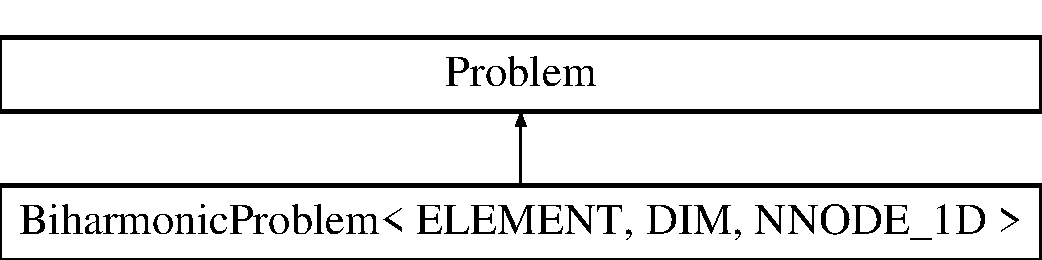
\includegraphics[height=2.000000cm]{classBiharmonicProblem}
\end{center}
\end{figure}
\subsection*{Public Member Functions}
\begin{DoxyCompactItemize}
\item 
\hyperlink{classBiharmonicProblem_a947d20f6658aa16bb92086a8ed025491}{Biharmonic\+Problem} (typename \hyperlink{classoomph_1_1MyBiharmonicEquations}{My\+Biharmonic\+Equations}$<$ D\+IM, N\+N\+O\+D\+E\+\_\+1D $>$\+::Source\+Fct\+Pt source\+\_\+fct\+\_\+pt, const string \&node\+\_\+file\+\_\+name, const string \&element\+\_\+file\+\_\+name, const string \&poly\+\_\+file\+\_\+name)
\begin{DoxyCompactList}\small\item\em Constructor\+: Pass number of elements and pointer to source function. \end{DoxyCompactList}\item 
\hyperlink{classBiharmonicProblem_aaa512f8c05170aa4a7b97e175db642f3}{$\sim$\+Biharmonic\+Problem} ()
\begin{DoxyCompactList}\small\item\em Destructor (empty) \end{DoxyCompactList}\item 
void \hyperlink{classBiharmonicProblem_ac159c323626ae0514dac820b3f1a2ffb}{actions\+\_\+before\+\_\+newton\+\_\+solve} ()
\begin{DoxyCompactList}\small\item\em Update the problem specs before solve\+: (Re)set boundary conditions. \end{DoxyCompactList}\item 
void \hyperlink{classBiharmonicProblem_ac48f3f4d5164572e711103d7c58de9ed}{actions\+\_\+after\+\_\+newton\+\_\+solve} ()
\begin{DoxyCompactList}\small\item\em Update the problem specs after solve (empty) \end{DoxyCompactList}\item 
void \hyperlink{classBiharmonicProblem_a0cb56f30738170a8d2bfd1c8d1000fd4}{doc\+\_\+solution} (Doc\+Info \&doc\+\_\+info)
\begin{DoxyCompactList}\small\item\em Doc the solution, pass the number of the case considered, so that output files can be distinguished. \end{DoxyCompactList}\end{DoxyCompactItemize}
\subsection*{Private Attributes}
\begin{DoxyCompactItemize}
\item 
\hyperlink{classoomph_1_1MyBiharmonicEquations}{My\+Biharmonic\+Equations}$<$ D\+IM, N\+N\+O\+D\+E\+\_\+1D $>$\+::Source\+Fct\+Pt \hyperlink{classBiharmonicProblem_a4e4e3dc027b6ccf7b0b4e519f84b0843}{Source\+\_\+fct\+\_\+pt}
\begin{DoxyCompactList}\small\item\em Pointer to source function. \end{DoxyCompactList}\end{DoxyCompactItemize}


\subsection{Detailed Description}
\subsubsection*{template$<$class E\+L\+E\+M\+E\+NT, unsigned D\+IM, unsigned N\+N\+O\+D\+E\+\_\+1D$>$\newline
class Biharmonic\+Problem$<$ E\+L\+E\+M\+E\+N\+T, D\+I\+M, N\+N\+O\+D\+E\+\_\+1\+D $>$}

2D Biharmonic problem. 

Definition at line 974 of file unstructured\+\_\+2d\+\_\+biharmonic\+\_\+bellelement.\+cc.



\subsection{Constructor \& Destructor Documentation}
\mbox{\Hypertarget{classBiharmonicProblem_a947d20f6658aa16bb92086a8ed025491}\label{classBiharmonicProblem_a947d20f6658aa16bb92086a8ed025491}} 
\index{Biharmonic\+Problem@{Biharmonic\+Problem}!Biharmonic\+Problem@{Biharmonic\+Problem}}
\index{Biharmonic\+Problem@{Biharmonic\+Problem}!Biharmonic\+Problem@{Biharmonic\+Problem}}
\subsubsection{\texorpdfstring{Biharmonic\+Problem()}{BiharmonicProblem()}}
{\footnotesize\ttfamily template$<$class E\+L\+E\+M\+E\+NT , unsigned D\+IM, unsigned N\+N\+O\+D\+E\+\_\+1D$>$ \\
\hyperlink{classBiharmonicProblem}{Biharmonic\+Problem}$<$ E\+L\+E\+M\+E\+NT, D\+IM, N\+N\+O\+D\+E\+\_\+1D $>$\+::\hyperlink{classBiharmonicProblem}{Biharmonic\+Problem} (\begin{DoxyParamCaption}\item[{typename \hyperlink{classoomph_1_1MyBiharmonicEquations}{My\+Biharmonic\+Equations}$<$ D\+IM, N\+N\+O\+D\+E\+\_\+1D $>$\+::Source\+Fct\+Pt}]{source\+\_\+fct\+\_\+pt,  }\item[{const string \&}]{node\+\_\+file\+\_\+name,  }\item[{const string \&}]{element\+\_\+file\+\_\+name,  }\item[{const string \&}]{poly\+\_\+file\+\_\+name }\end{DoxyParamCaption})}



Constructor\+: Pass number of elements and pointer to source function. 

Constructor for 2D Biharmonic problem. Discretise the 2D domain with n\+\_\+element elements of type E\+L\+E\+M\+E\+NT. Specify function pointer to source function. 

Definition at line 1016 of file unstructured\+\_\+2d\+\_\+biharmonic\+\_\+bellelement.\+cc.

\mbox{\Hypertarget{classBiharmonicProblem_aaa512f8c05170aa4a7b97e175db642f3}\label{classBiharmonicProblem_aaa512f8c05170aa4a7b97e175db642f3}} 
\index{Biharmonic\+Problem@{Biharmonic\+Problem}!````~Biharmonic\+Problem@{$\sim$\+Biharmonic\+Problem}}
\index{````~Biharmonic\+Problem@{$\sim$\+Biharmonic\+Problem}!Biharmonic\+Problem@{Biharmonic\+Problem}}
\subsubsection{\texorpdfstring{$\sim$\+Biharmonic\+Problem()}{~BiharmonicProblem()}}
{\footnotesize\ttfamily template$<$class E\+L\+E\+M\+E\+NT, unsigned D\+IM, unsigned N\+N\+O\+D\+E\+\_\+1D$>$ \\
\hyperlink{classBiharmonicProblem}{Biharmonic\+Problem}$<$ E\+L\+E\+M\+E\+NT, D\+IM, N\+N\+O\+D\+E\+\_\+1D $>$\+::$\sim$\hyperlink{classBiharmonicProblem}{Biharmonic\+Problem} (\begin{DoxyParamCaption}{ }\end{DoxyParamCaption})\hspace{0.3cm}{\ttfamily [inline]}}



Destructor (empty) 



Definition at line 985 of file unstructured\+\_\+2d\+\_\+biharmonic\+\_\+bellelement.\+cc.



\subsection{Member Function Documentation}
\mbox{\Hypertarget{classBiharmonicProblem_ac48f3f4d5164572e711103d7c58de9ed}\label{classBiharmonicProblem_ac48f3f4d5164572e711103d7c58de9ed}} 
\index{Biharmonic\+Problem@{Biharmonic\+Problem}!actions\+\_\+after\+\_\+newton\+\_\+solve@{actions\+\_\+after\+\_\+newton\+\_\+solve}}
\index{actions\+\_\+after\+\_\+newton\+\_\+solve@{actions\+\_\+after\+\_\+newton\+\_\+solve}!Biharmonic\+Problem@{Biharmonic\+Problem}}
\subsubsection{\texorpdfstring{actions\+\_\+after\+\_\+newton\+\_\+solve()}{actions\_after\_newton\_solve()}}
{\footnotesize\ttfamily template$<$class E\+L\+E\+M\+E\+NT, unsigned D\+IM, unsigned N\+N\+O\+D\+E\+\_\+1D$>$ \\
void \hyperlink{classBiharmonicProblem}{Biharmonic\+Problem}$<$ E\+L\+E\+M\+E\+NT, D\+IM, N\+N\+O\+D\+E\+\_\+1D $>$\+::actions\+\_\+after\+\_\+newton\+\_\+solve (\begin{DoxyParamCaption}{ }\end{DoxyParamCaption})\hspace{0.3cm}{\ttfamily [inline]}}



Update the problem specs after solve (empty) 



Definition at line 994 of file unstructured\+\_\+2d\+\_\+biharmonic\+\_\+bellelement.\+cc.

\mbox{\Hypertarget{classBiharmonicProblem_ac159c323626ae0514dac820b3f1a2ffb}\label{classBiharmonicProblem_ac159c323626ae0514dac820b3f1a2ffb}} 
\index{Biharmonic\+Problem@{Biharmonic\+Problem}!actions\+\_\+before\+\_\+newton\+\_\+solve@{actions\+\_\+before\+\_\+newton\+\_\+solve}}
\index{actions\+\_\+before\+\_\+newton\+\_\+solve@{actions\+\_\+before\+\_\+newton\+\_\+solve}!Biharmonic\+Problem@{Biharmonic\+Problem}}
\subsubsection{\texorpdfstring{actions\+\_\+before\+\_\+newton\+\_\+solve()}{actions\_before\_newton\_solve()}}
{\footnotesize\ttfamily template$<$class E\+L\+E\+M\+E\+NT , unsigned D\+IM, unsigned N\+N\+O\+D\+E\+\_\+1D$>$ \\
void \hyperlink{classBiharmonicProblem}{Biharmonic\+Problem}$<$ E\+L\+E\+M\+E\+NT, D\+IM, N\+N\+O\+D\+E\+\_\+1D $>$\+::actions\+\_\+before\+\_\+newton\+\_\+solve (\begin{DoxyParamCaption}{ }\end{DoxyParamCaption})}



Update the problem specs before solve\+: (Re)set boundary conditions. 

Update the problem specs before solve\+: (Re)set boundary values from the exact solution. 

Definition at line 1069 of file unstructured\+\_\+2d\+\_\+biharmonic\+\_\+bellelement.\+cc.



References Physical\+\_\+\+Variables\+::get\+\_\+exact\+\_\+u().

\mbox{\Hypertarget{classBiharmonicProblem_a0cb56f30738170a8d2bfd1c8d1000fd4}\label{classBiharmonicProblem_a0cb56f30738170a8d2bfd1c8d1000fd4}} 
\index{Biharmonic\+Problem@{Biharmonic\+Problem}!doc\+\_\+solution@{doc\+\_\+solution}}
\index{doc\+\_\+solution@{doc\+\_\+solution}!Biharmonic\+Problem@{Biharmonic\+Problem}}
\subsubsection{\texorpdfstring{doc\+\_\+solution()}{doc\_solution()}}
{\footnotesize\ttfamily template$<$class E\+L\+E\+M\+E\+NT , unsigned D\+IM, unsigned N\+N\+O\+D\+E\+\_\+1D$>$ \\
void \hyperlink{classBiharmonicProblem}{Biharmonic\+Problem}$<$ E\+L\+E\+M\+E\+NT, D\+IM, N\+N\+O\+D\+E\+\_\+1D $>$\+::doc\+\_\+solution (\begin{DoxyParamCaption}\item[{Doc\+Info \&}]{doc\+\_\+info }\end{DoxyParamCaption})}



Doc the solution, pass the number of the case considered, so that output files can be distinguished. 

Doc the solution in tecplot format. Label files with label. 

Definition at line 1110 of file unstructured\+\_\+2d\+\_\+biharmonic\+\_\+bellelement.\+cc.



References Physical\+\_\+\+Variables\+::get\+\_\+exact\+\_\+u().



Referenced by main().



\subsection{Member Data Documentation}
\mbox{\Hypertarget{classBiharmonicProblem_a4e4e3dc027b6ccf7b0b4e519f84b0843}\label{classBiharmonicProblem_a4e4e3dc027b6ccf7b0b4e519f84b0843}} 
\index{Biharmonic\+Problem@{Biharmonic\+Problem}!Source\+\_\+fct\+\_\+pt@{Source\+\_\+fct\+\_\+pt}}
\index{Source\+\_\+fct\+\_\+pt@{Source\+\_\+fct\+\_\+pt}!Biharmonic\+Problem@{Biharmonic\+Problem}}
\subsubsection{\texorpdfstring{Source\+\_\+fct\+\_\+pt}{Source\_fct\_pt}}
{\footnotesize\ttfamily template$<$class E\+L\+E\+M\+E\+NT, unsigned D\+IM, unsigned N\+N\+O\+D\+E\+\_\+1D$>$ \\
\hyperlink{classoomph_1_1MyBiharmonicEquations}{My\+Biharmonic\+Equations}$<$D\+IM,N\+N\+O\+D\+E\+\_\+1D$>$\+::Source\+Fct\+Pt \hyperlink{classBiharmonicProblem}{Biharmonic\+Problem}$<$ E\+L\+E\+M\+E\+NT, D\+IM, N\+N\+O\+D\+E\+\_\+1D $>$\+::Source\+\_\+fct\+\_\+pt\hspace{0.3cm}{\ttfamily [private]}}



Pointer to source function. 



Definition at line 1003 of file unstructured\+\_\+2d\+\_\+biharmonic\+\_\+bellelement.\+cc.



The documentation for this class was generated from the following file\+:\begin{DoxyCompactItemize}
\item 
\hyperlink{unstructured__2d__biharmonic__bellelement_8cc}{unstructured\+\_\+2d\+\_\+biharmonic\+\_\+bellelement.\+cc}\end{DoxyCompactItemize}

\hypertarget{classoomph_1_1FaceGeometry_3_01BellBiharmonicElement_3_01DIM_00_01NNODE__1D_01_4_01_4}{}\section{oomph\+:\+:Face\+Geometry$<$ Bell\+Biharmonic\+Element$<$ D\+IM, N\+N\+O\+D\+E\+\_\+1D $>$ $>$ Class Template Reference}
\label{classoomph_1_1FaceGeometry_3_01BellBiharmonicElement_3_01DIM_00_01NNODE__1D_01_4_01_4}\index{oomph\+::\+Face\+Geometry$<$ Bell\+Biharmonic\+Element$<$ D\+I\+M, N\+N\+O\+D\+E\+\_\+1\+D $>$ $>$@{oomph\+::\+Face\+Geometry$<$ Bell\+Biharmonic\+Element$<$ D\+I\+M, N\+N\+O\+D\+E\+\_\+1\+D $>$ $>$}}
Inheritance diagram for oomph\+:\+:Face\+Geometry$<$ Bell\+Biharmonic\+Element$<$ D\+IM, N\+N\+O\+D\+E\+\_\+1D $>$ $>$\+:\begin{figure}[H]
\begin{center}
\leavevmode
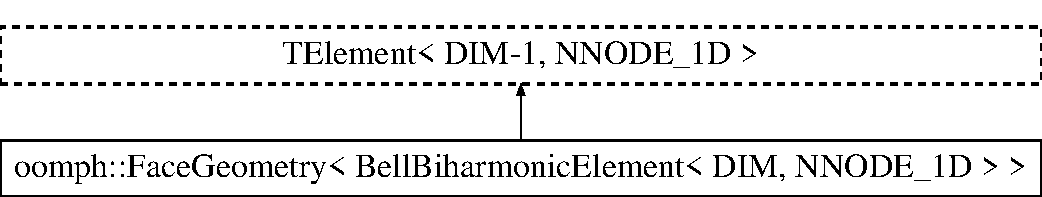
\includegraphics[height=2.000000cm]{classoomph_1_1FaceGeometry_3_01BellBiharmonicElement_3_01DIM_00_01NNODE__1D_01_4_01_4}
\end{center}
\end{figure}
\subsection*{Public Member Functions}
\begin{DoxyCompactItemize}
\item 
\hyperlink{classoomph_1_1FaceGeometry_3_01BellBiharmonicElement_3_01DIM_00_01NNODE__1D_01_4_01_4_a9242ac70d699ed140af2d89299b9cf19}{Face\+Geometry} ()
\begin{DoxyCompactList}\small\item\em Constructor\+: Call the constructor for the appropriate lower-\/dimensional T\+Element. \end{DoxyCompactList}\end{DoxyCompactItemize}


\subsection{Detailed Description}
\subsubsection*{template$<$unsigned D\+IM, unsigned N\+N\+O\+D\+E\+\_\+1D$>$\newline
class oomph\+::\+Face\+Geometry$<$ Bell\+Biharmonic\+Element$<$ D\+I\+M, N\+N\+O\+D\+E\+\_\+1\+D $>$ $>$}

Face geometry for the \hyperlink{classoomph_1_1BellBiharmonicElement}{Bell\+Biharmonic\+Element} elements\+: The spatial dimension of the face elements is one lower than that of the bulk element but they have the same number of points along their 1D edges. 

Definition at line 427 of file unstructured\+\_\+2d\+\_\+biharmonic\+\_\+bellelement.\+cc.



\subsection{Constructor \& Destructor Documentation}
\mbox{\Hypertarget{classoomph_1_1FaceGeometry_3_01BellBiharmonicElement_3_01DIM_00_01NNODE__1D_01_4_01_4_a9242ac70d699ed140af2d89299b9cf19}\label{classoomph_1_1FaceGeometry_3_01BellBiharmonicElement_3_01DIM_00_01NNODE__1D_01_4_01_4_a9242ac70d699ed140af2d89299b9cf19}} 
\index{oomph\+::\+Face\+Geometry$<$ Bell\+Biharmonic\+Element$<$ D\+I\+M, N\+N\+O\+D\+E\+\_\+1\+D $>$ $>$@{oomph\+::\+Face\+Geometry$<$ Bell\+Biharmonic\+Element$<$ D\+I\+M, N\+N\+O\+D\+E\+\_\+1\+D $>$ $>$}!Face\+Geometry@{Face\+Geometry}}
\index{Face\+Geometry@{Face\+Geometry}!oomph\+::\+Face\+Geometry$<$ Bell\+Biharmonic\+Element$<$ D\+I\+M, N\+N\+O\+D\+E\+\_\+1\+D $>$ $>$@{oomph\+::\+Face\+Geometry$<$ Bell\+Biharmonic\+Element$<$ D\+I\+M, N\+N\+O\+D\+E\+\_\+1\+D $>$ $>$}}
\subsubsection{\texorpdfstring{Face\+Geometry()}{FaceGeometry()}}
{\footnotesize\ttfamily template$<$unsigned D\+IM, unsigned N\+N\+O\+D\+E\+\_\+1D$>$ \\
oomph\+::\+Face\+Geometry$<$ \hyperlink{classoomph_1_1BellBiharmonicElement}{Bell\+Biharmonic\+Element}$<$ D\+IM, N\+N\+O\+D\+E\+\_\+1D $>$ $>$\+::Face\+Geometry (\begin{DoxyParamCaption}{ }\end{DoxyParamCaption})\hspace{0.3cm}{\ttfamily [inline]}}



Constructor\+: Call the constructor for the appropriate lower-\/dimensional T\+Element. 



Definition at line 435 of file unstructured\+\_\+2d\+\_\+biharmonic\+\_\+bellelement.\+cc.



The documentation for this class was generated from the following file\+:\begin{DoxyCompactItemize}
\item 
\hyperlink{unstructured__2d__biharmonic__bellelement_8cc}{unstructured\+\_\+2d\+\_\+biharmonic\+\_\+bellelement.\+cc}\end{DoxyCompactItemize}

\hypertarget{classoomph_1_1FaceGeometry_3_01BiharmonicCurvedElement_3_01DIM_00_01NNODE__1D_01_4_01_4}{}\section{oomph\+:\+:Face\+Geometry$<$ Biharmonic\+Curved\+Element$<$ D\+IM, N\+N\+O\+D\+E\+\_\+1D $>$ $>$ Class Template Reference}
\label{classoomph_1_1FaceGeometry_3_01BiharmonicCurvedElement_3_01DIM_00_01NNODE__1D_01_4_01_4}\index{oomph\+::\+Face\+Geometry$<$ Biharmonic\+Curved\+Element$<$ D\+I\+M, N\+N\+O\+D\+E\+\_\+1\+D $>$ $>$@{oomph\+::\+Face\+Geometry$<$ Biharmonic\+Curved\+Element$<$ D\+I\+M, N\+N\+O\+D\+E\+\_\+1\+D $>$ $>$}}
Inheritance diagram for oomph\+:\+:Face\+Geometry$<$ Biharmonic\+Curved\+Element$<$ D\+IM, N\+N\+O\+D\+E\+\_\+1D $>$ $>$\+:\begin{figure}[H]
\begin{center}
\leavevmode
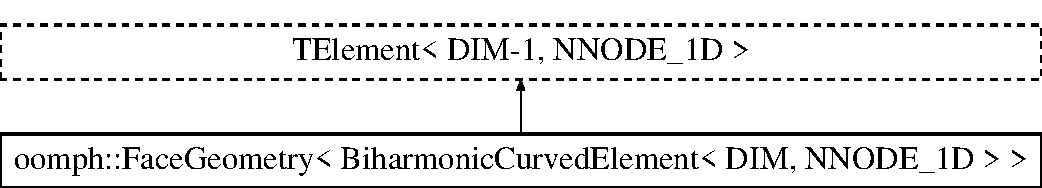
\includegraphics[height=2.000000cm]{classoomph_1_1FaceGeometry_3_01BiharmonicCurvedElement_3_01DIM_00_01NNODE__1D_01_4_01_4}
\end{center}
\end{figure}
\subsection*{Public Member Functions}
\begin{DoxyCompactItemize}
\item 
\hyperlink{classoomph_1_1FaceGeometry_3_01BiharmonicCurvedElement_3_01DIM_00_01NNODE__1D_01_4_01_4_a9b53ebab89d9c273519b2cd4b338a898}{Face\+Geometry} ()
\begin{DoxyCompactList}\small\item\em Constructor\+: Call the constructor for the appropriate lower-\/dimensional T\+Element. \end{DoxyCompactList}\end{DoxyCompactItemize}


\subsection{Detailed Description}
\subsubsection*{template$<$unsigned D\+IM, unsigned N\+N\+O\+D\+E\+\_\+1D$>$\newline
class oomph\+::\+Face\+Geometry$<$ Biharmonic\+Curved\+Element$<$ D\+I\+M, N\+N\+O\+D\+E\+\_\+1\+D $>$ $>$}

Face geometry for the Curved\+T\+Element elements\+: The spatial dimension of the face elements is one lower than that of the bulk element but they have the same number of points along their 1D edges. 

Definition at line 445 of file unstructured\+\_\+2d\+\_\+biharmonic\+\_\+curvedelement.\+cc.



\subsection{Constructor \& Destructor Documentation}
\mbox{\Hypertarget{classoomph_1_1FaceGeometry_3_01BiharmonicCurvedElement_3_01DIM_00_01NNODE__1D_01_4_01_4_a9b53ebab89d9c273519b2cd4b338a898}\label{classoomph_1_1FaceGeometry_3_01BiharmonicCurvedElement_3_01DIM_00_01NNODE__1D_01_4_01_4_a9b53ebab89d9c273519b2cd4b338a898}} 
\index{oomph\+::\+Face\+Geometry$<$ Biharmonic\+Curved\+Element$<$ D\+I\+M, N\+N\+O\+D\+E\+\_\+1\+D $>$ $>$@{oomph\+::\+Face\+Geometry$<$ Biharmonic\+Curved\+Element$<$ D\+I\+M, N\+N\+O\+D\+E\+\_\+1\+D $>$ $>$}!Face\+Geometry@{Face\+Geometry}}
\index{Face\+Geometry@{Face\+Geometry}!oomph\+::\+Face\+Geometry$<$ Biharmonic\+Curved\+Element$<$ D\+I\+M, N\+N\+O\+D\+E\+\_\+1\+D $>$ $>$@{oomph\+::\+Face\+Geometry$<$ Biharmonic\+Curved\+Element$<$ D\+I\+M, N\+N\+O\+D\+E\+\_\+1\+D $>$ $>$}}
\subsubsection{\texorpdfstring{Face\+Geometry()}{FaceGeometry()}}
{\footnotesize\ttfamily template$<$unsigned D\+IM, unsigned N\+N\+O\+D\+E\+\_\+1D$>$ \\
oomph\+::\+Face\+Geometry$<$ \hyperlink{classoomph_1_1BiharmonicCurvedElement}{Biharmonic\+Curved\+Element}$<$ D\+IM, N\+N\+O\+D\+E\+\_\+1D $>$ $>$\+::Face\+Geometry (\begin{DoxyParamCaption}{ }\end{DoxyParamCaption})\hspace{0.3cm}{\ttfamily [inline]}}



Constructor\+: Call the constructor for the appropriate lower-\/dimensional T\+Element. 



Definition at line 453 of file unstructured\+\_\+2d\+\_\+biharmonic\+\_\+curvedelement.\+cc.



The documentation for this class was generated from the following file\+:\begin{DoxyCompactItemize}
\item 
\hyperlink{unstructured__2d__biharmonic__curvedelement_8cc}{unstructured\+\_\+2d\+\_\+biharmonic\+\_\+curvedelement.\+cc}\end{DoxyCompactItemize}

\hypertarget{classoomph_1_1MyBiharmonicEquations}{}\section{oomph\+:\+:My\+Biharmonic\+Equations$<$ D\+IM, N\+N\+O\+D\+E\+\_\+1D $>$ Class Template Reference}
\label{classoomph_1_1MyBiharmonicEquations}\index{oomph\+::\+My\+Biharmonic\+Equations$<$ D\+I\+M, N\+N\+O\+D\+E\+\_\+1\+D $>$@{oomph\+::\+My\+Biharmonic\+Equations$<$ D\+I\+M, N\+N\+O\+D\+E\+\_\+1\+D $>$}}
Inheritance diagram for oomph\+:\+:My\+Biharmonic\+Equations$<$ D\+IM, N\+N\+O\+D\+E\+\_\+1D $>$\+:\begin{figure}[H]
\begin{center}
\leavevmode
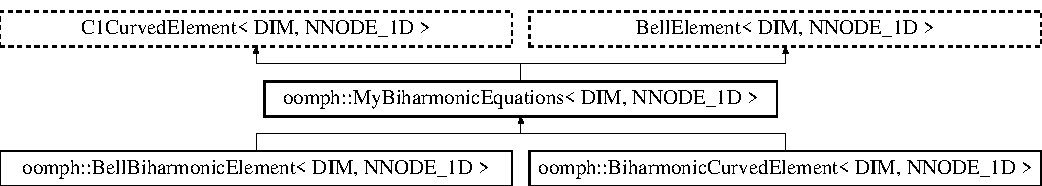
\includegraphics[height=3.000000cm]{classoomph_1_1MyBiharmonicEquations}
\end{center}
\end{figure}
\subsection*{Public Types}
\begin{DoxyCompactItemize}
\item 
typedef void($\ast$ \hyperlink{classoomph_1_1MyBiharmonicEquations_a17bd58054c66229016eb1c52eab36bc1}{Source\+Fct\+Pt}) (const Vector$<$ double $>$ \&x, double \&f)
\begin{DoxyCompactList}\small\item\em Function pointer to source function fct(x,f(x)) -- x is a Vector! \end{DoxyCompactList}\item 
typedef void($\ast$ \hyperlink{classoomph_1_1MyBiharmonicEquations_af007c03701e888fed7375cb4537f0046}{Source\+Fct\+Gradient\+Pt}) (const Vector$<$ double $>$ \&x, Vector$<$ double $>$ \&gradient)
\begin{DoxyCompactList}\small\item\em Function pointer to gradient of source function fct(x,g(x)) -- x is a Vector! \end{DoxyCompactList}\end{DoxyCompactItemize}
\subsection*{Public Member Functions}
\begin{DoxyCompactItemize}
\item 
\hyperlink{classoomph_1_1MyBiharmonicEquations_ab5084decf9d75cee91f0e88fb4f62c86}{My\+Biharmonic\+Equations} ()
\begin{DoxyCompactList}\small\item\em Constructor (must initialise the Source\+\_\+fct\+\_\+pt to null) \end{DoxyCompactList}\item 
\hyperlink{classoomph_1_1MyBiharmonicEquations_a3cf0e0a63e46219b94195aa4ab926316}{My\+Biharmonic\+Equations} (const \hyperlink{classoomph_1_1MyBiharmonicEquations}{My\+Biharmonic\+Equations} \&dummy)
\begin{DoxyCompactList}\small\item\em Broken copy constructor. \end{DoxyCompactList}\item 
virtual unsigned \hyperlink{classoomph_1_1MyBiharmonicEquations_aecad5ed2e1534519b81e778c5dff6457}{u\+\_\+index\+\_\+biharmonic} () const
\begin{DoxyCompactList}\small\item\em Return the index at which the unknown value is stored. The default value, 0, is appropriate for single-\/physics problems, when there is only one variable, the value that satisfies the biharmonic equation. In derived multi-\/physics elements, this function should be overloaded to reflect the chosen storage scheme. Note that these equations require that the unknown is always stored at the same index at each node. \end{DoxyCompactList}\item 
void \hyperlink{classoomph_1_1MyBiharmonicEquations_aa0d1248dcc8fcebd986c295d6af2ebf6}{output} (std\+::ostream \&outfile)
\begin{DoxyCompactList}\small\item\em Output with default number of plot points. \end{DoxyCompactList}\item 
void \hyperlink{classoomph_1_1MyBiharmonicEquations_a9a2734695e94f83eb6d553a7090dbebd}{output} (std\+::ostream \&outfile, const unsigned \&n\+\_\+plot)
\begin{DoxyCompactList}\small\item\em Output FE representation of soln\+: x,y,u or x,y,z,u at n\+\_\+plot$^\wedge$\+D\+IM plot points. \end{DoxyCompactList}\item 
void \hyperlink{classoomph_1_1MyBiharmonicEquations_a2ee8f210f50cf3b43f2b31b5e16b704f}{output} (F\+I\+LE $\ast$file\+\_\+pt)
\begin{DoxyCompactList}\small\item\em C\+\_\+style output with default number of plot points. \end{DoxyCompactList}\item 
void \hyperlink{classoomph_1_1MyBiharmonicEquations_a898e272a1af66eacb3ebe5ac2fbe7749}{output} (F\+I\+LE $\ast$file\+\_\+pt, const unsigned \&n\+\_\+plot)
\begin{DoxyCompactList}\small\item\em C-\/style output FE representation of soln\+: x,y,u or x,y,z,u at n\+\_\+plot$^\wedge$\+D\+IM plot points. \end{DoxyCompactList}\item 
void \hyperlink{classoomph_1_1MyBiharmonicEquations_a0f45f28eae4d25ddd9e53a769c3626a3}{output\+\_\+fct} (std\+::ostream \&outfile, const unsigned \&n\+\_\+plot, Finite\+Element\+::\+Steady\+Exact\+Solution\+Fct\+Pt exact\+\_\+soln\+\_\+pt)
\begin{DoxyCompactList}\small\item\em Output exact soln\+: x,y,u\+\_\+exact or x,y,z,u\+\_\+exact at n\+\_\+plot$^\wedge$\+D\+IM plot points. \end{DoxyCompactList}\item 
virtual void \hyperlink{classoomph_1_1MyBiharmonicEquations_a95b35b18fac5212ade1a81c26657bcdb}{output\+\_\+fct} (std\+::ostream \&outfile, const unsigned \&n\+\_\+plot, const double \&time, Finite\+Element\+::\+Unsteady\+Exact\+Solution\+Fct\+Pt exact\+\_\+soln\+\_\+pt)
\begin{DoxyCompactList}\small\item\em Output exact soln\+: x,y,u\+\_\+exact or x,y,z,u\+\_\+exact at n\+\_\+plot$^\wedge$\+D\+IM plot points (dummy time-\/dependent version to keep intel compiler happy) \end{DoxyCompactList}\item 
void \hyperlink{classoomph_1_1MyBiharmonicEquations_ac605d044c4e8c0483dcdf9b3b9e6634d}{compute\+\_\+error} (std\+::ostream \&outfile, Finite\+Element\+::\+Steady\+Exact\+Solution\+Fct\+Pt exact\+\_\+soln\+\_\+pt, double \&error, double \&norm)
\begin{DoxyCompactList}\small\item\em Get error against and norm of exact solution. \end{DoxyCompactList}\item 
void \hyperlink{classoomph_1_1MyBiharmonicEquations_a617b8c8dc3dbac7aeb9d466f6da4edb9}{compute\+\_\+error} (std\+::ostream \&outfile, Finite\+Element\+::\+Unsteady\+Exact\+Solution\+Fct\+Pt exact\+\_\+soln\+\_\+pt, const double \&time, double \&error, double \&norm)
\begin{DoxyCompactList}\small\item\em Dummy, time dependent error checker. \end{DoxyCompactList}\item 
\hyperlink{classoomph_1_1MyBiharmonicEquations_a17bd58054c66229016eb1c52eab36bc1}{Source\+Fct\+Pt} \& \hyperlink{classoomph_1_1MyBiharmonicEquations_afbb201cb342fef337cfce82a776fa2b3}{source\+\_\+fct\+\_\+pt} ()
\begin{DoxyCompactList}\small\item\em Access function\+: Pointer to source function. \end{DoxyCompactList}\item 
\hyperlink{classoomph_1_1MyBiharmonicEquations_a17bd58054c66229016eb1c52eab36bc1}{Source\+Fct\+Pt} \hyperlink{classoomph_1_1MyBiharmonicEquations_a1c2d7933266cf773e3729fb236bc13be}{source\+\_\+fct\+\_\+pt} () const
\begin{DoxyCompactList}\small\item\em Access function\+: Pointer to source function. Const version. \end{DoxyCompactList}\item 
\hyperlink{classoomph_1_1MyBiharmonicEquations_af007c03701e888fed7375cb4537f0046}{Source\+Fct\+Gradient\+Pt} \& \hyperlink{classoomph_1_1MyBiharmonicEquations_a9da77a58e4d4a96e6cfe1eb708bca631}{source\+\_\+fct\+\_\+gradient\+\_\+pt} ()
\begin{DoxyCompactList}\small\item\em Access function\+: Pointer to gradient of source function. \end{DoxyCompactList}\item 
\hyperlink{classoomph_1_1MyBiharmonicEquations_af007c03701e888fed7375cb4537f0046}{Source\+Fct\+Gradient\+Pt} \hyperlink{classoomph_1_1MyBiharmonicEquations_a3c6a713fdc0847a374c58ef4760046ec}{source\+\_\+fct\+\_\+gradient\+\_\+pt} () const
\begin{DoxyCompactList}\small\item\em Access function\+: Pointer to gradient source function. Const version. \end{DoxyCompactList}\item 
virtual void \hyperlink{classoomph_1_1MyBiharmonicEquations_a30d824f604ff00b823238d5b18561693}{get\+\_\+source\+\_\+function} (const unsigned \&ipt, const Vector$<$ double $>$ \&x, double \&source) const
\item 
void \hyperlink{classoomph_1_1MyBiharmonicEquations_a2f795bb316c3a9fc749639a8d3f8b5dd}{fill\+\_\+in\+\_\+contribution\+\_\+to\+\_\+residuals} (Vector$<$ double $>$ \&residuals)
\begin{DoxyCompactList}\small\item\em Add the element\textquotesingle{}s contribution to its residual vector (wrapper) \end{DoxyCompactList}\item 
void \hyperlink{classoomph_1_1MyBiharmonicEquations_ad5ef6af62c0ebf27bacf62be8d408c8a}{fill\+\_\+in\+\_\+contribution\+\_\+to\+\_\+jacobian} (Vector$<$ double $>$ \&residuals, Dense\+Matrix$<$ double $>$ \&jacobian)
\item 
Vector$<$ double $>$ \hyperlink{classoomph_1_1MyBiharmonicEquations_ac451e7d6ebf1dd94f0a0c122e3882d53}{interpolated\+\_\+u\+\_\+biharmonic} (const Vector$<$ double $>$ \&s) const
\begin{DoxyCompactList}\small\item\em Return FE representation of function value unknown(s) at local coordinate s. \end{DoxyCompactList}\item 
unsigned \hyperlink{classoomph_1_1MyBiharmonicEquations_a6898ff065e57f8e765440da81075cf3d}{self\+\_\+test} ()
\begin{DoxyCompactList}\small\item\em Self-\/test\+: Return 0 for OK. \end{DoxyCompactList}\end{DoxyCompactItemize}
\subsection*{Protected Member Functions}
\begin{DoxyCompactItemize}
\item 
virtual double \hyperlink{classoomph_1_1MyBiharmonicEquations_a4597b3938b6f1244d6e8e0f58250c14a}{d2shape\+\_\+and\+\_\+d2test\+\_\+eulerian\+\_\+biharmonic} (const Vector$<$ double $>$ \&s, Shape \&psi, D\+Shape \&dpsidx, D\+Shape \&d2psidx, Shape \&test, D\+Shape \&dtestdx, D\+Shape \&d2testdx) const =0
\begin{DoxyCompactList}\small\item\em Shape/test functions and derivs w.\+r.\+t. to global coords at local coord. s; return Jacobian of mapping. \end{DoxyCompactList}\item 
virtual double \hyperlink{classoomph_1_1MyBiharmonicEquations_a084eaadd62185dad622c7708862f023a}{dshape\+\_\+and\+\_\+dtest\+\_\+eulerian\+\_\+biharmonic} (const Vector$<$ double $>$ \&s, Shape \&psi, D\+Shape \&dpsidx, Shape \&test, D\+Shape \&dtestdx) const =0
\item 
virtual double \hyperlink{classoomph_1_1MyBiharmonicEquations_a85687f39c0fb72f25ce67f5867a83470}{d2shape\+\_\+and\+\_\+d2test\+\_\+eulerian\+\_\+at\+\_\+knot\+\_\+biharmonic} (const unsigned \&ipt, Shape \&psi, D\+Shape \&dpsidx, D\+Shape \&d2psidx, Shape \&test, D\+Shape \&dtestdx, D\+Shape \&d2testdx) const =0
\begin{DoxyCompactList}\small\item\em Shape/test functions and derivs w.\+r.\+t. to global coords at integration point ipt; return Jacobian of mapping. \end{DoxyCompactList}\item 
virtual double \hyperlink{classoomph_1_1MyBiharmonicEquations_a08e45fddb2c25119e6ba826cd6cafdbf}{dshape\+\_\+and\+\_\+dtest\+\_\+eulerian\+\_\+at\+\_\+knot\+\_\+biharmonic} (const unsigned \&ipt, Shape \&psi, D\+Shape \&dpsidx, Shape \&test, D\+Shape \&dtestdx) const =0
\item 
virtual void \hyperlink{classoomph_1_1MyBiharmonicEquations_ad951338582f7807eb83999e09f7486ec}{fill\+\_\+in\+\_\+generic\+\_\+residual\+\_\+contribution} (Vector$<$ double $>$ \&residuals, Dense\+Matrix$<$ double $>$ \&jacobian, const unsigned \&flag)
\begin{DoxyCompactList}\small\item\em Compute element residual Vector only (if flag=and/or element Jacobian matrix. \end{DoxyCompactList}\end{DoxyCompactItemize}
\subsection*{Protected Attributes}
\begin{DoxyCompactItemize}
\item 
\hyperlink{classoomph_1_1MyBiharmonicEquations_a17bd58054c66229016eb1c52eab36bc1}{Source\+Fct\+Pt} \hyperlink{classoomph_1_1MyBiharmonicEquations_aa96fd779e04f5c726f2535f43210e905}{Source\+\_\+fct\+\_\+pt}
\begin{DoxyCompactList}\small\item\em Pointer to source function\+: \end{DoxyCompactList}\item 
\hyperlink{classoomph_1_1MyBiharmonicEquations_af007c03701e888fed7375cb4537f0046}{Source\+Fct\+Gradient\+Pt} \hyperlink{classoomph_1_1MyBiharmonicEquations_afbd71d4a6c31f36d88bf60697c4140aa}{Source\+\_\+fct\+\_\+gradient\+\_\+pt}
\begin{DoxyCompactList}\small\item\em Pointer to gradient of source function. \end{DoxyCompactList}\end{DoxyCompactItemize}


\subsection{Detailed Description}
\subsubsection*{template$<$unsigned D\+IM, unsigned N\+N\+O\+D\+E\+\_\+1D$>$\newline
class oomph\+::\+My\+Biharmonic\+Equations$<$ D\+I\+M, N\+N\+O\+D\+E\+\_\+1\+D $>$}

A class for all subparametric elements that solve the 2\+D-\/ Biharmonic equations. \[ \frac{\partial^4 u}{\partial x_i^4} = f(x_j) \] This contains the generic maths. Shape functions, geometric mapping etc. must get implemented in derived class. 

Definition at line 68 of file structured\+\_\+2d\+\_\+biharmonic\+\_\+bellelement.\+cc.



\subsection{Member Typedef Documentation}
\mbox{\Hypertarget{classoomph_1_1MyBiharmonicEquations_af007c03701e888fed7375cb4537f0046}\label{classoomph_1_1MyBiharmonicEquations_af007c03701e888fed7375cb4537f0046}} 
\index{oomph\+::\+My\+Biharmonic\+Equations@{oomph\+::\+My\+Biharmonic\+Equations}!Source\+Fct\+Gradient\+Pt@{Source\+Fct\+Gradient\+Pt}}
\index{Source\+Fct\+Gradient\+Pt@{Source\+Fct\+Gradient\+Pt}!oomph\+::\+My\+Biharmonic\+Equations@{oomph\+::\+My\+Biharmonic\+Equations}}
\subsubsection{\texorpdfstring{Source\+Fct\+Gradient\+Pt}{SourceFctGradientPt}}
{\footnotesize\ttfamily template$<$unsigned D\+IM, unsigned N\+N\+O\+D\+E\+\_\+1D$>$ \\
typedef void($\ast$ \hyperlink{classoomph_1_1MyBiharmonicEquations}{oomph\+::\+My\+Biharmonic\+Equations}$<$ D\+IM, N\+N\+O\+D\+E\+\_\+1D $>$\+::Source\+Fct\+Gradient\+Pt) (const Vector$<$ double $>$ \&x, Vector$<$ double $>$ \&gradient)}



Function pointer to gradient of source function fct(x,g(x)) -- x is a Vector! 



Definition at line 80 of file structured\+\_\+2d\+\_\+biharmonic\+\_\+bellelement.\+cc.

\mbox{\Hypertarget{classoomph_1_1MyBiharmonicEquations_a17bd58054c66229016eb1c52eab36bc1}\label{classoomph_1_1MyBiharmonicEquations_a17bd58054c66229016eb1c52eab36bc1}} 
\index{oomph\+::\+My\+Biharmonic\+Equations@{oomph\+::\+My\+Biharmonic\+Equations}!Source\+Fct\+Pt@{Source\+Fct\+Pt}}
\index{Source\+Fct\+Pt@{Source\+Fct\+Pt}!oomph\+::\+My\+Biharmonic\+Equations@{oomph\+::\+My\+Biharmonic\+Equations}}
\subsubsection{\texorpdfstring{Source\+Fct\+Pt}{SourceFctPt}}
{\footnotesize\ttfamily template$<$unsigned D\+IM, unsigned N\+N\+O\+D\+E\+\_\+1D$>$ \\
typedef void($\ast$ \hyperlink{classoomph_1_1MyBiharmonicEquations}{oomph\+::\+My\+Biharmonic\+Equations}$<$ D\+IM, N\+N\+O\+D\+E\+\_\+1D $>$\+::Source\+Fct\+Pt) (const Vector$<$ double $>$ \&x, double \&f)}



Function pointer to source function fct(x,f(x)) -- x is a Vector! 



Definition at line 75 of file structured\+\_\+2d\+\_\+biharmonic\+\_\+bellelement.\+cc.



\subsection{Constructor \& Destructor Documentation}
\mbox{\Hypertarget{classoomph_1_1MyBiharmonicEquations_ab5084decf9d75cee91f0e88fb4f62c86}\label{classoomph_1_1MyBiharmonicEquations_ab5084decf9d75cee91f0e88fb4f62c86}} 
\index{oomph\+::\+My\+Biharmonic\+Equations@{oomph\+::\+My\+Biharmonic\+Equations}!My\+Biharmonic\+Equations@{My\+Biharmonic\+Equations}}
\index{My\+Biharmonic\+Equations@{My\+Biharmonic\+Equations}!oomph\+::\+My\+Biharmonic\+Equations@{oomph\+::\+My\+Biharmonic\+Equations}}
\subsubsection{\texorpdfstring{My\+Biharmonic\+Equations()}{MyBiharmonicEquations()}\hspace{0.1cm}{\footnotesize\ttfamily [1/2]}}
{\footnotesize\ttfamily template$<$unsigned D\+IM, unsigned N\+N\+O\+D\+E\+\_\+1D$>$ \\
\hyperlink{classoomph_1_1MyBiharmonicEquations}{oomph\+::\+My\+Biharmonic\+Equations}$<$ D\+IM, N\+N\+O\+D\+E\+\_\+1D $>$\+::\hyperlink{classoomph_1_1MyBiharmonicEquations}{My\+Biharmonic\+Equations} (\begin{DoxyParamCaption}{ }\end{DoxyParamCaption})\hspace{0.3cm}{\ttfamily [inline]}}



Constructor (must initialise the Source\+\_\+fct\+\_\+pt to null) 



Definition at line 85 of file structured\+\_\+2d\+\_\+biharmonic\+\_\+bellelement.\+cc.

\mbox{\Hypertarget{classoomph_1_1MyBiharmonicEquations_a3cf0e0a63e46219b94195aa4ab926316}\label{classoomph_1_1MyBiharmonicEquations_a3cf0e0a63e46219b94195aa4ab926316}} 
\index{oomph\+::\+My\+Biharmonic\+Equations@{oomph\+::\+My\+Biharmonic\+Equations}!My\+Biharmonic\+Equations@{My\+Biharmonic\+Equations}}
\index{My\+Biharmonic\+Equations@{My\+Biharmonic\+Equations}!oomph\+::\+My\+Biharmonic\+Equations@{oomph\+::\+My\+Biharmonic\+Equations}}
\subsubsection{\texorpdfstring{My\+Biharmonic\+Equations()}{MyBiharmonicEquations()}\hspace{0.1cm}{\footnotesize\ttfamily [2/2]}}
{\footnotesize\ttfamily template$<$unsigned D\+IM, unsigned N\+N\+O\+D\+E\+\_\+1D$>$ \\
\hyperlink{classoomph_1_1MyBiharmonicEquations}{oomph\+::\+My\+Biharmonic\+Equations}$<$ D\+IM, N\+N\+O\+D\+E\+\_\+1D $>$\+::\hyperlink{classoomph_1_1MyBiharmonicEquations}{My\+Biharmonic\+Equations} (\begin{DoxyParamCaption}\item[{const \hyperlink{classoomph_1_1MyBiharmonicEquations}{My\+Biharmonic\+Equations}$<$ D\+IM, N\+N\+O\+D\+E\+\_\+1D $>$ \&}]{dummy }\end{DoxyParamCaption})\hspace{0.3cm}{\ttfamily [inline]}}



Broken copy constructor. 



Definition at line 89 of file structured\+\_\+2d\+\_\+biharmonic\+\_\+bellelement.\+cc.



\subsection{Member Function Documentation}
\mbox{\Hypertarget{classoomph_1_1MyBiharmonicEquations_ac605d044c4e8c0483dcdf9b3b9e6634d}\label{classoomph_1_1MyBiharmonicEquations_ac605d044c4e8c0483dcdf9b3b9e6634d}} 
\index{oomph\+::\+My\+Biharmonic\+Equations@{oomph\+::\+My\+Biharmonic\+Equations}!compute\+\_\+error@{compute\+\_\+error}}
\index{compute\+\_\+error@{compute\+\_\+error}!oomph\+::\+My\+Biharmonic\+Equations@{oomph\+::\+My\+Biharmonic\+Equations}}
\subsubsection{\texorpdfstring{compute\+\_\+error()}{compute\_error()}\hspace{0.1cm}{\footnotesize\ttfamily [1/2]}}
{\footnotesize\ttfamily template$<$unsigned D\+IM, unsigned N\+N\+O\+D\+E\+\_\+1D$>$ \\
void \hyperlink{classoomph_1_1MyBiharmonicEquations}{oomph\+::\+My\+Biharmonic\+Equations}$<$ D\+IM, N\+N\+O\+D\+E\+\_\+1D $>$\+::compute\+\_\+error (\begin{DoxyParamCaption}\item[{std\+::ostream \&}]{outfile,  }\item[{Finite\+Element\+::\+Steady\+Exact\+Solution\+Fct\+Pt}]{exact\+\_\+soln\+\_\+pt,  }\item[{double \&}]{error,  }\item[{double \&}]{norm }\end{DoxyParamCaption})}



Get error against and norm of exact solution. 

Validate against exact solution

Solution is provided via function pointer. Plot error at a given number of plot points. 

Definition at line 835 of file structured\+\_\+2d\+\_\+biharmonic\+\_\+bellelement.\+cc.

\mbox{\Hypertarget{classoomph_1_1MyBiharmonicEquations_a617b8c8dc3dbac7aeb9d466f6da4edb9}\label{classoomph_1_1MyBiharmonicEquations_a617b8c8dc3dbac7aeb9d466f6da4edb9}} 
\index{oomph\+::\+My\+Biharmonic\+Equations@{oomph\+::\+My\+Biharmonic\+Equations}!compute\+\_\+error@{compute\+\_\+error}}
\index{compute\+\_\+error@{compute\+\_\+error}!oomph\+::\+My\+Biharmonic\+Equations@{oomph\+::\+My\+Biharmonic\+Equations}}
\subsubsection{\texorpdfstring{compute\+\_\+error()}{compute\_error()}\hspace{0.1cm}{\footnotesize\ttfamily [2/2]}}
{\footnotesize\ttfamily template$<$unsigned D\+IM, unsigned N\+N\+O\+D\+E\+\_\+1D$>$ \\
void \hyperlink{classoomph_1_1MyBiharmonicEquations}{oomph\+::\+My\+Biharmonic\+Equations}$<$ D\+IM, N\+N\+O\+D\+E\+\_\+1D $>$\+::compute\+\_\+error (\begin{DoxyParamCaption}\item[{std\+::ostream \&}]{outfile,  }\item[{Finite\+Element\+::\+Unsteady\+Exact\+Solution\+Fct\+Pt}]{exact\+\_\+soln\+\_\+pt,  }\item[{const double \&}]{time,  }\item[{double \&}]{error,  }\item[{double \&}]{norm }\end{DoxyParamCaption})\hspace{0.3cm}{\ttfamily [inline]}}



Dummy, time dependent error checker. 



Definition at line 151 of file structured\+\_\+2d\+\_\+biharmonic\+\_\+bellelement.\+cc.

\mbox{\Hypertarget{classoomph_1_1MyBiharmonicEquations_a85687f39c0fb72f25ce67f5867a83470}\label{classoomph_1_1MyBiharmonicEquations_a85687f39c0fb72f25ce67f5867a83470}} 
\index{oomph\+::\+My\+Biharmonic\+Equations@{oomph\+::\+My\+Biharmonic\+Equations}!d2shape\+\_\+and\+\_\+d2test\+\_\+eulerian\+\_\+at\+\_\+knot\+\_\+biharmonic@{d2shape\+\_\+and\+\_\+d2test\+\_\+eulerian\+\_\+at\+\_\+knot\+\_\+biharmonic}}
\index{d2shape\+\_\+and\+\_\+d2test\+\_\+eulerian\+\_\+at\+\_\+knot\+\_\+biharmonic@{d2shape\+\_\+and\+\_\+d2test\+\_\+eulerian\+\_\+at\+\_\+knot\+\_\+biharmonic}!oomph\+::\+My\+Biharmonic\+Equations@{oomph\+::\+My\+Biharmonic\+Equations}}
\subsubsection{\texorpdfstring{d2shape\+\_\+and\+\_\+d2test\+\_\+eulerian\+\_\+at\+\_\+knot\+\_\+biharmonic()}{d2shape\_and\_d2test\_eulerian\_at\_knot\_biharmonic()}}
{\footnotesize\ttfamily template$<$unsigned D\+IM, unsigned N\+N\+O\+D\+E\+\_\+1D$>$ \\
virtual double \hyperlink{classoomph_1_1MyBiharmonicEquations}{oomph\+::\+My\+Biharmonic\+Equations}$<$ D\+IM, N\+N\+O\+D\+E\+\_\+1D $>$\+::d2shape\+\_\+and\+\_\+d2test\+\_\+eulerian\+\_\+at\+\_\+knot\+\_\+biharmonic (\begin{DoxyParamCaption}\item[{const unsigned \&}]{ipt,  }\item[{Shape \&}]{psi,  }\item[{D\+Shape \&}]{dpsidx,  }\item[{D\+Shape \&}]{d2psidx,  }\item[{Shape \&}]{test,  }\item[{D\+Shape \&}]{dtestdx,  }\item[{D\+Shape \&}]{d2testdx }\end{DoxyParamCaption}) const\hspace{0.3cm}{\ttfamily [protected]}, {\ttfamily [pure virtual]}}



Shape/test functions and derivs w.\+r.\+t. to global coords at integration point ipt; return Jacobian of mapping. 



Implemented in \hyperlink{classoomph_1_1BiharmonicBellElement_a5a98ec12400b72d5fd31e62c6c250339}{oomph\+::\+Biharmonic\+Bell\+Element$<$ D\+I\+M, N\+N\+O\+D\+E\+\_\+1\+D $>$}.

\mbox{\Hypertarget{classoomph_1_1MyBiharmonicEquations_a4597b3938b6f1244d6e8e0f58250c14a}\label{classoomph_1_1MyBiharmonicEquations_a4597b3938b6f1244d6e8e0f58250c14a}} 
\index{oomph\+::\+My\+Biharmonic\+Equations@{oomph\+::\+My\+Biharmonic\+Equations}!d2shape\+\_\+and\+\_\+d2test\+\_\+eulerian\+\_\+biharmonic@{d2shape\+\_\+and\+\_\+d2test\+\_\+eulerian\+\_\+biharmonic}}
\index{d2shape\+\_\+and\+\_\+d2test\+\_\+eulerian\+\_\+biharmonic@{d2shape\+\_\+and\+\_\+d2test\+\_\+eulerian\+\_\+biharmonic}!oomph\+::\+My\+Biharmonic\+Equations@{oomph\+::\+My\+Biharmonic\+Equations}}
\subsubsection{\texorpdfstring{d2shape\+\_\+and\+\_\+d2test\+\_\+eulerian\+\_\+biharmonic()}{d2shape\_and\_d2test\_eulerian\_biharmonic()}}
{\footnotesize\ttfamily template$<$unsigned D\+IM, unsigned N\+N\+O\+D\+E\+\_\+1D$>$ \\
virtual double \hyperlink{classoomph_1_1MyBiharmonicEquations}{oomph\+::\+My\+Biharmonic\+Equations}$<$ D\+IM, N\+N\+O\+D\+E\+\_\+1D $>$\+::d2shape\+\_\+and\+\_\+d2test\+\_\+eulerian\+\_\+biharmonic (\begin{DoxyParamCaption}\item[{const Vector$<$ double $>$ \&}]{s,  }\item[{Shape \&}]{psi,  }\item[{D\+Shape \&}]{dpsidx,  }\item[{D\+Shape \&}]{d2psidx,  }\item[{Shape \&}]{test,  }\item[{D\+Shape \&}]{dtestdx,  }\item[{D\+Shape \&}]{d2testdx }\end{DoxyParamCaption}) const\hspace{0.3cm}{\ttfamily [protected]}, {\ttfamily [pure virtual]}}



Shape/test functions and derivs w.\+r.\+t. to global coords at local coord. s; return Jacobian of mapping. 



Implemented in \hyperlink{classoomph_1_1BiharmonicBellElement_ac0343916d2900e138d5d5e98aa46b758}{oomph\+::\+Biharmonic\+Bell\+Element$<$ D\+I\+M, N\+N\+O\+D\+E\+\_\+1\+D $>$}.

\mbox{\Hypertarget{classoomph_1_1MyBiharmonicEquations_a08e45fddb2c25119e6ba826cd6cafdbf}\label{classoomph_1_1MyBiharmonicEquations_a08e45fddb2c25119e6ba826cd6cafdbf}} 
\index{oomph\+::\+My\+Biharmonic\+Equations@{oomph\+::\+My\+Biharmonic\+Equations}!dshape\+\_\+and\+\_\+dtest\+\_\+eulerian\+\_\+at\+\_\+knot\+\_\+biharmonic@{dshape\+\_\+and\+\_\+dtest\+\_\+eulerian\+\_\+at\+\_\+knot\+\_\+biharmonic}}
\index{dshape\+\_\+and\+\_\+dtest\+\_\+eulerian\+\_\+at\+\_\+knot\+\_\+biharmonic@{dshape\+\_\+and\+\_\+dtest\+\_\+eulerian\+\_\+at\+\_\+knot\+\_\+biharmonic}!oomph\+::\+My\+Biharmonic\+Equations@{oomph\+::\+My\+Biharmonic\+Equations}}
\subsubsection{\texorpdfstring{dshape\+\_\+and\+\_\+dtest\+\_\+eulerian\+\_\+at\+\_\+knot\+\_\+biharmonic()}{dshape\_and\_dtest\_eulerian\_at\_knot\_biharmonic()}}
{\footnotesize\ttfamily template$<$unsigned D\+IM, unsigned N\+N\+O\+D\+E\+\_\+1D$>$ \\
virtual double \hyperlink{classoomph_1_1MyBiharmonicEquations}{oomph\+::\+My\+Biharmonic\+Equations}$<$ D\+IM, N\+N\+O\+D\+E\+\_\+1D $>$\+::dshape\+\_\+and\+\_\+dtest\+\_\+eulerian\+\_\+at\+\_\+knot\+\_\+biharmonic (\begin{DoxyParamCaption}\item[{const unsigned \&}]{ipt,  }\item[{Shape \&}]{psi,  }\item[{D\+Shape \&}]{dpsidx,  }\item[{Shape \&}]{test,  }\item[{D\+Shape \&}]{dtestdx }\end{DoxyParamCaption}) const\hspace{0.3cm}{\ttfamily [protected]}, {\ttfamily [pure virtual]}}



Implemented in \hyperlink{classoomph_1_1BiharmonicBellElement_ab15a039def500f435638bed6f02edbcb}{oomph\+::\+Biharmonic\+Bell\+Element$<$ D\+I\+M, N\+N\+O\+D\+E\+\_\+1\+D $>$}.

\mbox{\Hypertarget{classoomph_1_1MyBiharmonicEquations_a084eaadd62185dad622c7708862f023a}\label{classoomph_1_1MyBiharmonicEquations_a084eaadd62185dad622c7708862f023a}} 
\index{oomph\+::\+My\+Biharmonic\+Equations@{oomph\+::\+My\+Biharmonic\+Equations}!dshape\+\_\+and\+\_\+dtest\+\_\+eulerian\+\_\+biharmonic@{dshape\+\_\+and\+\_\+dtest\+\_\+eulerian\+\_\+biharmonic}}
\index{dshape\+\_\+and\+\_\+dtest\+\_\+eulerian\+\_\+biharmonic@{dshape\+\_\+and\+\_\+dtest\+\_\+eulerian\+\_\+biharmonic}!oomph\+::\+My\+Biharmonic\+Equations@{oomph\+::\+My\+Biharmonic\+Equations}}
\subsubsection{\texorpdfstring{dshape\+\_\+and\+\_\+dtest\+\_\+eulerian\+\_\+biharmonic()}{dshape\_and\_dtest\_eulerian\_biharmonic()}}
{\footnotesize\ttfamily template$<$unsigned D\+IM, unsigned N\+N\+O\+D\+E\+\_\+1D$>$ \\
virtual double \hyperlink{classoomph_1_1MyBiharmonicEquations}{oomph\+::\+My\+Biharmonic\+Equations}$<$ D\+IM, N\+N\+O\+D\+E\+\_\+1D $>$\+::dshape\+\_\+and\+\_\+dtest\+\_\+eulerian\+\_\+biharmonic (\begin{DoxyParamCaption}\item[{const Vector$<$ double $>$ \&}]{s,  }\item[{Shape \&}]{psi,  }\item[{D\+Shape \&}]{dpsidx,  }\item[{Shape \&}]{test,  }\item[{D\+Shape \&}]{dtestdx }\end{DoxyParamCaption}) const\hspace{0.3cm}{\ttfamily [protected]}, {\ttfamily [pure virtual]}}



Implemented in \hyperlink{classoomph_1_1BiharmonicBellElement_ab4fc981e180b12acd2a9865efb42459b}{oomph\+::\+Biharmonic\+Bell\+Element$<$ D\+I\+M, N\+N\+O\+D\+E\+\_\+1\+D $>$}.

\mbox{\Hypertarget{classoomph_1_1MyBiharmonicEquations_ad5ef6af62c0ebf27bacf62be8d408c8a}\label{classoomph_1_1MyBiharmonicEquations_ad5ef6af62c0ebf27bacf62be8d408c8a}} 
\index{oomph\+::\+My\+Biharmonic\+Equations@{oomph\+::\+My\+Biharmonic\+Equations}!fill\+\_\+in\+\_\+contribution\+\_\+to\+\_\+jacobian@{fill\+\_\+in\+\_\+contribution\+\_\+to\+\_\+jacobian}}
\index{fill\+\_\+in\+\_\+contribution\+\_\+to\+\_\+jacobian@{fill\+\_\+in\+\_\+contribution\+\_\+to\+\_\+jacobian}!oomph\+::\+My\+Biharmonic\+Equations@{oomph\+::\+My\+Biharmonic\+Equations}}
\subsubsection{\texorpdfstring{fill\+\_\+in\+\_\+contribution\+\_\+to\+\_\+jacobian()}{fill\_in\_contribution\_to\_jacobian()}}
{\footnotesize\ttfamily template$<$unsigned D\+IM, unsigned N\+N\+O\+D\+E\+\_\+1D$>$ \\
void \hyperlink{classoomph_1_1MyBiharmonicEquations}{oomph\+::\+My\+Biharmonic\+Equations}$<$ D\+IM, N\+N\+O\+D\+E\+\_\+1D $>$\+::fill\+\_\+in\+\_\+contribution\+\_\+to\+\_\+jacobian (\begin{DoxyParamCaption}\item[{Vector$<$ double $>$ \&}]{residuals,  }\item[{Dense\+Matrix$<$ double $>$ \&}]{jacobian }\end{DoxyParamCaption})\hspace{0.3cm}{\ttfamily [inline]}}

Add the element\textquotesingle{}s contribution to its residual vector and element Jacobian matrix (wrapper) 

Definition at line 207 of file structured\+\_\+2d\+\_\+biharmonic\+\_\+bellelement.\+cc.

\mbox{\Hypertarget{classoomph_1_1MyBiharmonicEquations_a2f795bb316c3a9fc749639a8d3f8b5dd}\label{classoomph_1_1MyBiharmonicEquations_a2f795bb316c3a9fc749639a8d3f8b5dd}} 
\index{oomph\+::\+My\+Biharmonic\+Equations@{oomph\+::\+My\+Biharmonic\+Equations}!fill\+\_\+in\+\_\+contribution\+\_\+to\+\_\+residuals@{fill\+\_\+in\+\_\+contribution\+\_\+to\+\_\+residuals}}
\index{fill\+\_\+in\+\_\+contribution\+\_\+to\+\_\+residuals@{fill\+\_\+in\+\_\+contribution\+\_\+to\+\_\+residuals}!oomph\+::\+My\+Biharmonic\+Equations@{oomph\+::\+My\+Biharmonic\+Equations}}
\subsubsection{\texorpdfstring{fill\+\_\+in\+\_\+contribution\+\_\+to\+\_\+residuals()}{fill\_in\_contribution\_to\_residuals()}}
{\footnotesize\ttfamily template$<$unsigned D\+IM, unsigned N\+N\+O\+D\+E\+\_\+1D$>$ \\
void \hyperlink{classoomph_1_1MyBiharmonicEquations}{oomph\+::\+My\+Biharmonic\+Equations}$<$ D\+IM, N\+N\+O\+D\+E\+\_\+1D $>$\+::fill\+\_\+in\+\_\+contribution\+\_\+to\+\_\+residuals (\begin{DoxyParamCaption}\item[{Vector$<$ double $>$ \&}]{residuals }\end{DoxyParamCaption})\hspace{0.3cm}{\ttfamily [inline]}}



Add the element\textquotesingle{}s contribution to its residual vector (wrapper) 



Definition at line 197 of file structured\+\_\+2d\+\_\+biharmonic\+\_\+bellelement.\+cc.

\mbox{\Hypertarget{classoomph_1_1MyBiharmonicEquations_ad951338582f7807eb83999e09f7486ec}\label{classoomph_1_1MyBiharmonicEquations_ad951338582f7807eb83999e09f7486ec}} 
\index{oomph\+::\+My\+Biharmonic\+Equations@{oomph\+::\+My\+Biharmonic\+Equations}!fill\+\_\+in\+\_\+generic\+\_\+residual\+\_\+contribution@{fill\+\_\+in\+\_\+generic\+\_\+residual\+\_\+contribution}}
\index{fill\+\_\+in\+\_\+generic\+\_\+residual\+\_\+contribution@{fill\+\_\+in\+\_\+generic\+\_\+residual\+\_\+contribution}!oomph\+::\+My\+Biharmonic\+Equations@{oomph\+::\+My\+Biharmonic\+Equations}}
\subsubsection{\texorpdfstring{fill\+\_\+in\+\_\+generic\+\_\+residual\+\_\+contribution()}{fill\_in\_generic\_residual\_contribution()}}
{\footnotesize\ttfamily template$<$unsigned D\+IM, unsigned N\+N\+O\+D\+E\+\_\+1D$>$ \\
void \hyperlink{classoomph_1_1MyBiharmonicEquations}{oomph\+::\+My\+Biharmonic\+Equations}$<$ D\+IM, N\+N\+O\+D\+E\+\_\+1D $>$\+::fill\+\_\+in\+\_\+generic\+\_\+residual\+\_\+contribution (\begin{DoxyParamCaption}\item[{Vector$<$ double $>$ \&}]{residuals,  }\item[{Dense\+Matrix$<$ double $>$ \&}]{jacobian,  }\item[{const unsigned \&}]{flag }\end{DoxyParamCaption})\hspace{0.3cm}{\ttfamily [protected]}, {\ttfamily [virtual]}}



Compute element residual Vector only (if flag=and/or element Jacobian matrix. 



Definition at line 532 of file structured\+\_\+2d\+\_\+biharmonic\+\_\+bellelement.\+cc.

\mbox{\Hypertarget{classoomph_1_1MyBiharmonicEquations_a30d824f604ff00b823238d5b18561693}\label{classoomph_1_1MyBiharmonicEquations_a30d824f604ff00b823238d5b18561693}} 
\index{oomph\+::\+My\+Biharmonic\+Equations@{oomph\+::\+My\+Biharmonic\+Equations}!get\+\_\+source\+\_\+function@{get\+\_\+source\+\_\+function}}
\index{get\+\_\+source\+\_\+function@{get\+\_\+source\+\_\+function}!oomph\+::\+My\+Biharmonic\+Equations@{oomph\+::\+My\+Biharmonic\+Equations}}
\subsubsection{\texorpdfstring{get\+\_\+source\+\_\+function()}{get\_source\_function()}}
{\footnotesize\ttfamily template$<$unsigned D\+IM, unsigned N\+N\+O\+D\+E\+\_\+1D$>$ \\
virtual void \hyperlink{classoomph_1_1MyBiharmonicEquations}{oomph\+::\+My\+Biharmonic\+Equations}$<$ D\+IM, N\+N\+O\+D\+E\+\_\+1D $>$\+::get\+\_\+source\+\_\+function (\begin{DoxyParamCaption}\item[{const unsigned \&}]{ipt,  }\item[{const Vector$<$ double $>$ \&}]{x,  }\item[{double \&}]{source }\end{DoxyParamCaption}) const\hspace{0.3cm}{\ttfamily [inline]}, {\ttfamily [virtual]}}

Get source term at (Eulerian) position x. This function is virtual to allow overloading in multi-\/physics problems where the strength of the source function might be determined by another system of equations. 

Definition at line 180 of file structured\+\_\+2d\+\_\+biharmonic\+\_\+bellelement.\+cc.

\mbox{\Hypertarget{classoomph_1_1MyBiharmonicEquations_ac451e7d6ebf1dd94f0a0c122e3882d53}\label{classoomph_1_1MyBiharmonicEquations_ac451e7d6ebf1dd94f0a0c122e3882d53}} 
\index{oomph\+::\+My\+Biharmonic\+Equations@{oomph\+::\+My\+Biharmonic\+Equations}!interpolated\+\_\+u\+\_\+biharmonic@{interpolated\+\_\+u\+\_\+biharmonic}}
\index{interpolated\+\_\+u\+\_\+biharmonic@{interpolated\+\_\+u\+\_\+biharmonic}!oomph\+::\+My\+Biharmonic\+Equations@{oomph\+::\+My\+Biharmonic\+Equations}}
\subsubsection{\texorpdfstring{interpolated\+\_\+u\+\_\+biharmonic()}{interpolated\_u\_biharmonic()}}
{\footnotesize\ttfamily template$<$unsigned D\+IM, unsigned N\+N\+O\+D\+E\+\_\+1D$>$ \\
Vector$<$double$>$ \hyperlink{classoomph_1_1MyBiharmonicEquations}{oomph\+::\+My\+Biharmonic\+Equations}$<$ D\+IM, N\+N\+O\+D\+E\+\_\+1D $>$\+::interpolated\+\_\+u\+\_\+biharmonic (\begin{DoxyParamCaption}\item[{const Vector$<$ double $>$ \&}]{s }\end{DoxyParamCaption}) const\hspace{0.3cm}{\ttfamily [inline]}}



Return FE representation of function value unknown(s) at local coordinate s. 



Definition at line 216 of file structured\+\_\+2d\+\_\+biharmonic\+\_\+bellelement.\+cc.

\mbox{\Hypertarget{classoomph_1_1MyBiharmonicEquations_aa0d1248dcc8fcebd986c295d6af2ebf6}\label{classoomph_1_1MyBiharmonicEquations_aa0d1248dcc8fcebd986c295d6af2ebf6}} 
\index{oomph\+::\+My\+Biharmonic\+Equations@{oomph\+::\+My\+Biharmonic\+Equations}!output@{output}}
\index{output@{output}!oomph\+::\+My\+Biharmonic\+Equations@{oomph\+::\+My\+Biharmonic\+Equations}}
\subsubsection{\texorpdfstring{output()}{output()}\hspace{0.1cm}{\footnotesize\ttfamily [1/4]}}
{\footnotesize\ttfamily template$<$unsigned D\+IM, unsigned N\+N\+O\+D\+E\+\_\+1D$>$ \\
void \hyperlink{classoomph_1_1MyBiharmonicEquations}{oomph\+::\+My\+Biharmonic\+Equations}$<$ D\+IM, N\+N\+O\+D\+E\+\_\+1D $>$\+::output (\begin{DoxyParamCaption}\item[{std\+::ostream \&}]{outfile }\end{DoxyParamCaption})\hspace{0.3cm}{\ttfamily [inline]}}



Output with default number of plot points. 



Definition at line 104 of file structured\+\_\+2d\+\_\+biharmonic\+\_\+bellelement.\+cc.

\mbox{\Hypertarget{classoomph_1_1MyBiharmonicEquations_a9a2734695e94f83eb6d553a7090dbebd}\label{classoomph_1_1MyBiharmonicEquations_a9a2734695e94f83eb6d553a7090dbebd}} 
\index{oomph\+::\+My\+Biharmonic\+Equations@{oomph\+::\+My\+Biharmonic\+Equations}!output@{output}}
\index{output@{output}!oomph\+::\+My\+Biharmonic\+Equations@{oomph\+::\+My\+Biharmonic\+Equations}}
\subsubsection{\texorpdfstring{output()}{output()}\hspace{0.1cm}{\footnotesize\ttfamily [2/4]}}
{\footnotesize\ttfamily template$<$unsigned D\+IM, unsigned N\+N\+O\+D\+E\+\_\+1D$>$ \\
void \hyperlink{classoomph_1_1MyBiharmonicEquations}{oomph\+::\+My\+Biharmonic\+Equations}$<$ D\+IM, N\+N\+O\+D\+E\+\_\+1D $>$\+::output (\begin{DoxyParamCaption}\item[{std\+::ostream \&}]{outfile,  }\item[{const unsigned \&}]{nplot }\end{DoxyParamCaption})}



Output FE representation of soln\+: x,y,u or x,y,z,u at n\+\_\+plot$^\wedge$\+D\+IM plot points. 

Output function\+:

x,y,u or x,y,z,u

nplot points in each coordinate direction 

Definition at line 684 of file structured\+\_\+2d\+\_\+biharmonic\+\_\+bellelement.\+cc.

\mbox{\Hypertarget{classoomph_1_1MyBiharmonicEquations_a2ee8f210f50cf3b43f2b31b5e16b704f}\label{classoomph_1_1MyBiharmonicEquations_a2ee8f210f50cf3b43f2b31b5e16b704f}} 
\index{oomph\+::\+My\+Biharmonic\+Equations@{oomph\+::\+My\+Biharmonic\+Equations}!output@{output}}
\index{output@{output}!oomph\+::\+My\+Biharmonic\+Equations@{oomph\+::\+My\+Biharmonic\+Equations}}
\subsubsection{\texorpdfstring{output()}{output()}\hspace{0.1cm}{\footnotesize\ttfamily [3/4]}}
{\footnotesize\ttfamily template$<$unsigned D\+IM, unsigned N\+N\+O\+D\+E\+\_\+1D$>$ \\
void \hyperlink{classoomph_1_1MyBiharmonicEquations}{oomph\+::\+My\+Biharmonic\+Equations}$<$ D\+IM, N\+N\+O\+D\+E\+\_\+1D $>$\+::output (\begin{DoxyParamCaption}\item[{F\+I\+LE $\ast$}]{file\+\_\+pt }\end{DoxyParamCaption})\hspace{0.3cm}{\ttfamily [inline]}}



C\+\_\+style output with default number of plot points. 



Definition at line 115 of file structured\+\_\+2d\+\_\+biharmonic\+\_\+bellelement.\+cc.

\mbox{\Hypertarget{classoomph_1_1MyBiharmonicEquations_a898e272a1af66eacb3ebe5ac2fbe7749}\label{classoomph_1_1MyBiharmonicEquations_a898e272a1af66eacb3ebe5ac2fbe7749}} 
\index{oomph\+::\+My\+Biharmonic\+Equations@{oomph\+::\+My\+Biharmonic\+Equations}!output@{output}}
\index{output@{output}!oomph\+::\+My\+Biharmonic\+Equations@{oomph\+::\+My\+Biharmonic\+Equations}}
\subsubsection{\texorpdfstring{output()}{output()}\hspace{0.1cm}{\footnotesize\ttfamily [4/4]}}
{\footnotesize\ttfamily template$<$unsigned D\+IM, unsigned N\+N\+O\+D\+E\+\_\+1D$>$ \\
void \hyperlink{classoomph_1_1MyBiharmonicEquations}{oomph\+::\+My\+Biharmonic\+Equations}$<$ D\+IM, N\+N\+O\+D\+E\+\_\+1D $>$\+::output (\begin{DoxyParamCaption}\item[{F\+I\+LE $\ast$}]{file\+\_\+pt,  }\item[{const unsigned \&}]{nplot }\end{DoxyParamCaption})}



C-\/style output FE representation of soln\+: x,y,u or x,y,z,u at n\+\_\+plot$^\wedge$\+D\+IM plot points. 

C-\/style output function\+:

x,y,u or x,y,z,u

nplot points in each coordinate direction 

Definition at line 736 of file structured\+\_\+2d\+\_\+biharmonic\+\_\+bellelement.\+cc.

\mbox{\Hypertarget{classoomph_1_1MyBiharmonicEquations_a0f45f28eae4d25ddd9e53a769c3626a3}\label{classoomph_1_1MyBiharmonicEquations_a0f45f28eae4d25ddd9e53a769c3626a3}} 
\index{oomph\+::\+My\+Biharmonic\+Equations@{oomph\+::\+My\+Biharmonic\+Equations}!output\+\_\+fct@{output\+\_\+fct}}
\index{output\+\_\+fct@{output\+\_\+fct}!oomph\+::\+My\+Biharmonic\+Equations@{oomph\+::\+My\+Biharmonic\+Equations}}
\subsubsection{\texorpdfstring{output\+\_\+fct()}{output\_fct()}\hspace{0.1cm}{\footnotesize\ttfamily [1/2]}}
{\footnotesize\ttfamily template$<$unsigned D\+IM, unsigned N\+N\+O\+D\+E\+\_\+1D$>$ \\
void \hyperlink{classoomph_1_1MyBiharmonicEquations}{oomph\+::\+My\+Biharmonic\+Equations}$<$ D\+IM, N\+N\+O\+D\+E\+\_\+1D $>$\+::output\+\_\+fct (\begin{DoxyParamCaption}\item[{std\+::ostream \&}]{outfile,  }\item[{const unsigned \&}]{nplot,  }\item[{Finite\+Element\+::\+Steady\+Exact\+Solution\+Fct\+Pt}]{exact\+\_\+soln\+\_\+pt }\end{DoxyParamCaption})}



Output exact soln\+: x,y,u\+\_\+exact or x,y,z,u\+\_\+exact at n\+\_\+plot$^\wedge$\+D\+IM plot points. 

Output exact solution

Solution is provided via function pointer. Plot at a given number of plot points.

x,y,u\+\_\+exact or x,y,z,u\+\_\+exact 

Definition at line 776 of file structured\+\_\+2d\+\_\+biharmonic\+\_\+bellelement.\+cc.

\mbox{\Hypertarget{classoomph_1_1MyBiharmonicEquations_a95b35b18fac5212ade1a81c26657bcdb}\label{classoomph_1_1MyBiharmonicEquations_a95b35b18fac5212ade1a81c26657bcdb}} 
\index{oomph\+::\+My\+Biharmonic\+Equations@{oomph\+::\+My\+Biharmonic\+Equations}!output\+\_\+fct@{output\+\_\+fct}}
\index{output\+\_\+fct@{output\+\_\+fct}!oomph\+::\+My\+Biharmonic\+Equations@{oomph\+::\+My\+Biharmonic\+Equations}}
\subsubsection{\texorpdfstring{output\+\_\+fct()}{output\_fct()}\hspace{0.1cm}{\footnotesize\ttfamily [2/2]}}
{\footnotesize\ttfamily template$<$unsigned D\+IM, unsigned N\+N\+O\+D\+E\+\_\+1D$>$ \\
virtual void \hyperlink{classoomph_1_1MyBiharmonicEquations}{oomph\+::\+My\+Biharmonic\+Equations}$<$ D\+IM, N\+N\+O\+D\+E\+\_\+1D $>$\+::output\+\_\+fct (\begin{DoxyParamCaption}\item[{std\+::ostream \&}]{outfile,  }\item[{const unsigned \&}]{n\+\_\+plot,  }\item[{const double \&}]{time,  }\item[{Finite\+Element\+::\+Unsteady\+Exact\+Solution\+Fct\+Pt}]{exact\+\_\+soln\+\_\+pt }\end{DoxyParamCaption})\hspace{0.3cm}{\ttfamily [inline]}, {\ttfamily [virtual]}}



Output exact soln\+: x,y,u\+\_\+exact or x,y,z,u\+\_\+exact at n\+\_\+plot$^\wedge$\+D\+IM plot points (dummy time-\/dependent version to keep intel compiler happy) 



Reimplemented in \hyperlink{classoomph_1_1BiharmonicBellElement_ac383ee9d4eedfe0646062847af2a9b2e}{oomph\+::\+Biharmonic\+Bell\+Element$<$ D\+I\+M, N\+N\+O\+D\+E\+\_\+1\+D $>$}.



Definition at line 132 of file structured\+\_\+2d\+\_\+biharmonic\+\_\+bellelement.\+cc.

\mbox{\Hypertarget{classoomph_1_1MyBiharmonicEquations_a6898ff065e57f8e765440da81075cf3d}\label{classoomph_1_1MyBiharmonicEquations_a6898ff065e57f8e765440da81075cf3d}} 
\index{oomph\+::\+My\+Biharmonic\+Equations@{oomph\+::\+My\+Biharmonic\+Equations}!self\+\_\+test@{self\+\_\+test}}
\index{self\+\_\+test@{self\+\_\+test}!oomph\+::\+My\+Biharmonic\+Equations@{oomph\+::\+My\+Biharmonic\+Equations}}
\subsubsection{\texorpdfstring{self\+\_\+test()}{self\_test()}}
{\footnotesize\ttfamily template$<$unsigned D\+IM, unsigned N\+N\+O\+D\+E\+\_\+1D$>$ \\
unsigned \hyperlink{classoomph_1_1MyBiharmonicEquations}{oomph\+::\+My\+Biharmonic\+Equations}$<$ D\+IM, N\+N\+O\+D\+E\+\_\+1D $>$\+::self\+\_\+test (\begin{DoxyParamCaption}{ }\end{DoxyParamCaption})}



Self-\/test\+: Return 0 for OK. 



Definition at line 651 of file structured\+\_\+2d\+\_\+biharmonic\+\_\+bellelement.\+cc.

\mbox{\Hypertarget{classoomph_1_1MyBiharmonicEquations_a9da77a58e4d4a96e6cfe1eb708bca631}\label{classoomph_1_1MyBiharmonicEquations_a9da77a58e4d4a96e6cfe1eb708bca631}} 
\index{oomph\+::\+My\+Biharmonic\+Equations@{oomph\+::\+My\+Biharmonic\+Equations}!source\+\_\+fct\+\_\+gradient\+\_\+pt@{source\+\_\+fct\+\_\+gradient\+\_\+pt}}
\index{source\+\_\+fct\+\_\+gradient\+\_\+pt@{source\+\_\+fct\+\_\+gradient\+\_\+pt}!oomph\+::\+My\+Biharmonic\+Equations@{oomph\+::\+My\+Biharmonic\+Equations}}
\subsubsection{\texorpdfstring{source\+\_\+fct\+\_\+gradient\+\_\+pt()}{source\_fct\_gradient\_pt()}\hspace{0.1cm}{\footnotesize\ttfamily [1/2]}}
{\footnotesize\ttfamily template$<$unsigned D\+IM, unsigned N\+N\+O\+D\+E\+\_\+1D$>$ \\
\hyperlink{classoomph_1_1MyBiharmonicEquations_af007c03701e888fed7375cb4537f0046}{Source\+Fct\+Gradient\+Pt}\& \hyperlink{classoomph_1_1MyBiharmonicEquations}{oomph\+::\+My\+Biharmonic\+Equations}$<$ D\+IM, N\+N\+O\+D\+E\+\_\+1D $>$\+::source\+\_\+fct\+\_\+gradient\+\_\+pt (\begin{DoxyParamCaption}{ }\end{DoxyParamCaption})\hspace{0.3cm}{\ttfamily [inline]}}



Access function\+: Pointer to gradient of source function. 



Definition at line 168 of file structured\+\_\+2d\+\_\+biharmonic\+\_\+bellelement.\+cc.

\mbox{\Hypertarget{classoomph_1_1MyBiharmonicEquations_a3c6a713fdc0847a374c58ef4760046ec}\label{classoomph_1_1MyBiharmonicEquations_a3c6a713fdc0847a374c58ef4760046ec}} 
\index{oomph\+::\+My\+Biharmonic\+Equations@{oomph\+::\+My\+Biharmonic\+Equations}!source\+\_\+fct\+\_\+gradient\+\_\+pt@{source\+\_\+fct\+\_\+gradient\+\_\+pt}}
\index{source\+\_\+fct\+\_\+gradient\+\_\+pt@{source\+\_\+fct\+\_\+gradient\+\_\+pt}!oomph\+::\+My\+Biharmonic\+Equations@{oomph\+::\+My\+Biharmonic\+Equations}}
\subsubsection{\texorpdfstring{source\+\_\+fct\+\_\+gradient\+\_\+pt()}{source\_fct\_gradient\_pt()}\hspace{0.1cm}{\footnotesize\ttfamily [2/2]}}
{\footnotesize\ttfamily template$<$unsigned D\+IM, unsigned N\+N\+O\+D\+E\+\_\+1D$>$ \\
\hyperlink{classoomph_1_1MyBiharmonicEquations_af007c03701e888fed7375cb4537f0046}{Source\+Fct\+Gradient\+Pt} \hyperlink{classoomph_1_1MyBiharmonicEquations}{oomph\+::\+My\+Biharmonic\+Equations}$<$ D\+IM, N\+N\+O\+D\+E\+\_\+1D $>$\+::source\+\_\+fct\+\_\+gradient\+\_\+pt (\begin{DoxyParamCaption}{ }\end{DoxyParamCaption}) const\hspace{0.3cm}{\ttfamily [inline]}}



Access function\+: Pointer to gradient source function. Const version. 



Definition at line 172 of file structured\+\_\+2d\+\_\+biharmonic\+\_\+bellelement.\+cc.

\mbox{\Hypertarget{classoomph_1_1MyBiharmonicEquations_afbb201cb342fef337cfce82a776fa2b3}\label{classoomph_1_1MyBiharmonicEquations_afbb201cb342fef337cfce82a776fa2b3}} 
\index{oomph\+::\+My\+Biharmonic\+Equations@{oomph\+::\+My\+Biharmonic\+Equations}!source\+\_\+fct\+\_\+pt@{source\+\_\+fct\+\_\+pt}}
\index{source\+\_\+fct\+\_\+pt@{source\+\_\+fct\+\_\+pt}!oomph\+::\+My\+Biharmonic\+Equations@{oomph\+::\+My\+Biharmonic\+Equations}}
\subsubsection{\texorpdfstring{source\+\_\+fct\+\_\+pt()}{source\_fct\_pt()}\hspace{0.1cm}{\footnotesize\ttfamily [1/2]}}
{\footnotesize\ttfamily template$<$unsigned D\+IM, unsigned N\+N\+O\+D\+E\+\_\+1D$>$ \\
\hyperlink{classoomph_1_1MyBiharmonicEquations_a17bd58054c66229016eb1c52eab36bc1}{Source\+Fct\+Pt}\& \hyperlink{classoomph_1_1MyBiharmonicEquations}{oomph\+::\+My\+Biharmonic\+Equations}$<$ D\+IM, N\+N\+O\+D\+E\+\_\+1D $>$\+::source\+\_\+fct\+\_\+pt (\begin{DoxyParamCaption}{ }\end{DoxyParamCaption})\hspace{0.3cm}{\ttfamily [inline]}}



Access function\+: Pointer to source function. 



Definition at line 162 of file structured\+\_\+2d\+\_\+biharmonic\+\_\+bellelement.\+cc.

\mbox{\Hypertarget{classoomph_1_1MyBiharmonicEquations_a1c2d7933266cf773e3729fb236bc13be}\label{classoomph_1_1MyBiharmonicEquations_a1c2d7933266cf773e3729fb236bc13be}} 
\index{oomph\+::\+My\+Biharmonic\+Equations@{oomph\+::\+My\+Biharmonic\+Equations}!source\+\_\+fct\+\_\+pt@{source\+\_\+fct\+\_\+pt}}
\index{source\+\_\+fct\+\_\+pt@{source\+\_\+fct\+\_\+pt}!oomph\+::\+My\+Biharmonic\+Equations@{oomph\+::\+My\+Biharmonic\+Equations}}
\subsubsection{\texorpdfstring{source\+\_\+fct\+\_\+pt()}{source\_fct\_pt()}\hspace{0.1cm}{\footnotesize\ttfamily [2/2]}}
{\footnotesize\ttfamily template$<$unsigned D\+IM, unsigned N\+N\+O\+D\+E\+\_\+1D$>$ \\
\hyperlink{classoomph_1_1MyBiharmonicEquations_a17bd58054c66229016eb1c52eab36bc1}{Source\+Fct\+Pt} \hyperlink{classoomph_1_1MyBiharmonicEquations}{oomph\+::\+My\+Biharmonic\+Equations}$<$ D\+IM, N\+N\+O\+D\+E\+\_\+1D $>$\+::source\+\_\+fct\+\_\+pt (\begin{DoxyParamCaption}{ }\end{DoxyParamCaption}) const\hspace{0.3cm}{\ttfamily [inline]}}



Access function\+: Pointer to source function. Const version. 



Definition at line 165 of file structured\+\_\+2d\+\_\+biharmonic\+\_\+bellelement.\+cc.

\mbox{\Hypertarget{classoomph_1_1MyBiharmonicEquations_aecad5ed2e1534519b81e778c5dff6457}\label{classoomph_1_1MyBiharmonicEquations_aecad5ed2e1534519b81e778c5dff6457}} 
\index{oomph\+::\+My\+Biharmonic\+Equations@{oomph\+::\+My\+Biharmonic\+Equations}!u\+\_\+index\+\_\+biharmonic@{u\+\_\+index\+\_\+biharmonic}}
\index{u\+\_\+index\+\_\+biharmonic@{u\+\_\+index\+\_\+biharmonic}!oomph\+::\+My\+Biharmonic\+Equations@{oomph\+::\+My\+Biharmonic\+Equations}}
\subsubsection{\texorpdfstring{u\+\_\+index\+\_\+biharmonic()}{u\_index\_biharmonic()}}
{\footnotesize\ttfamily template$<$unsigned D\+IM, unsigned N\+N\+O\+D\+E\+\_\+1D$>$ \\
virtual unsigned \hyperlink{classoomph_1_1MyBiharmonicEquations}{oomph\+::\+My\+Biharmonic\+Equations}$<$ D\+IM, N\+N\+O\+D\+E\+\_\+1D $>$\+::u\+\_\+index\+\_\+biharmonic (\begin{DoxyParamCaption}{ }\end{DoxyParamCaption}) const\hspace{0.3cm}{\ttfamily [inline]}, {\ttfamily [virtual]}}



Return the index at which the unknown value is stored. The default value, 0, is appropriate for single-\/physics problems, when there is only one variable, the value that satisfies the biharmonic equation. In derived multi-\/physics elements, this function should be overloaded to reflect the chosen storage scheme. Note that these equations require that the unknown is always stored at the same index at each node. 



Definition at line 101 of file structured\+\_\+2d\+\_\+biharmonic\+\_\+bellelement.\+cc.



\subsection{Member Data Documentation}
\mbox{\Hypertarget{classoomph_1_1MyBiharmonicEquations_afbd71d4a6c31f36d88bf60697c4140aa}\label{classoomph_1_1MyBiharmonicEquations_afbd71d4a6c31f36d88bf60697c4140aa}} 
\index{oomph\+::\+My\+Biharmonic\+Equations@{oomph\+::\+My\+Biharmonic\+Equations}!Source\+\_\+fct\+\_\+gradient\+\_\+pt@{Source\+\_\+fct\+\_\+gradient\+\_\+pt}}
\index{Source\+\_\+fct\+\_\+gradient\+\_\+pt@{Source\+\_\+fct\+\_\+gradient\+\_\+pt}!oomph\+::\+My\+Biharmonic\+Equations@{oomph\+::\+My\+Biharmonic\+Equations}}
\subsubsection{\texorpdfstring{Source\+\_\+fct\+\_\+gradient\+\_\+pt}{Source\_fct\_gradient\_pt}}
{\footnotesize\ttfamily template$<$unsigned D\+IM, unsigned N\+N\+O\+D\+E\+\_\+1D$>$ \\
\hyperlink{classoomph_1_1MyBiharmonicEquations_af007c03701e888fed7375cb4537f0046}{Source\+Fct\+Gradient\+Pt} \hyperlink{classoomph_1_1MyBiharmonicEquations}{oomph\+::\+My\+Biharmonic\+Equations}$<$ D\+IM, N\+N\+O\+D\+E\+\_\+1D $>$\+::Source\+\_\+fct\+\_\+gradient\+\_\+pt\hspace{0.3cm}{\ttfamily [protected]}}



Pointer to gradient of source function. 



Definition at line 298 of file structured\+\_\+2d\+\_\+biharmonic\+\_\+bellelement.\+cc.

\mbox{\Hypertarget{classoomph_1_1MyBiharmonicEquations_aa96fd779e04f5c726f2535f43210e905}\label{classoomph_1_1MyBiharmonicEquations_aa96fd779e04f5c726f2535f43210e905}} 
\index{oomph\+::\+My\+Biharmonic\+Equations@{oomph\+::\+My\+Biharmonic\+Equations}!Source\+\_\+fct\+\_\+pt@{Source\+\_\+fct\+\_\+pt}}
\index{Source\+\_\+fct\+\_\+pt@{Source\+\_\+fct\+\_\+pt}!oomph\+::\+My\+Biharmonic\+Equations@{oomph\+::\+My\+Biharmonic\+Equations}}
\subsubsection{\texorpdfstring{Source\+\_\+fct\+\_\+pt}{Source\_fct\_pt}}
{\footnotesize\ttfamily template$<$unsigned D\+IM, unsigned N\+N\+O\+D\+E\+\_\+1D$>$ \\
\hyperlink{classoomph_1_1MyBiharmonicEquations_a17bd58054c66229016eb1c52eab36bc1}{Source\+Fct\+Pt} \hyperlink{classoomph_1_1MyBiharmonicEquations}{oomph\+::\+My\+Biharmonic\+Equations}$<$ D\+IM, N\+N\+O\+D\+E\+\_\+1D $>$\+::Source\+\_\+fct\+\_\+pt\hspace{0.3cm}{\ttfamily [protected]}}



Pointer to source function\+: 



Definition at line 295 of file structured\+\_\+2d\+\_\+biharmonic\+\_\+bellelement.\+cc.



The documentation for this class was generated from the following file\+:\begin{DoxyCompactItemize}
\item 
\hyperlink{structured__2d__biharmonic__bellelement_8cc}{structured\+\_\+2d\+\_\+biharmonic\+\_\+bellelement.\+cc}\end{DoxyCompactItemize}

\hypertarget{classMyBiharmonicProblem}{}\section{My\+Biharmonic\+Problem$<$ E\+L\+E\+M\+E\+NT, D\+IM, N\+N\+O\+D\+E\+\_\+1D $>$ Class Template Reference}
\label{classMyBiharmonicProblem}\index{My\+Biharmonic\+Problem$<$ E\+L\+E\+M\+E\+N\+T, D\+I\+M, N\+N\+O\+D\+E\+\_\+1\+D $>$@{My\+Biharmonic\+Problem$<$ E\+L\+E\+M\+E\+N\+T, D\+I\+M, N\+N\+O\+D\+E\+\_\+1\+D $>$}}


2D Biharmonic problem.  


Inheritance diagram for My\+Biharmonic\+Problem$<$ E\+L\+E\+M\+E\+NT, D\+IM, N\+N\+O\+D\+E\+\_\+1D $>$\+:\begin{figure}[H]
\begin{center}
\leavevmode
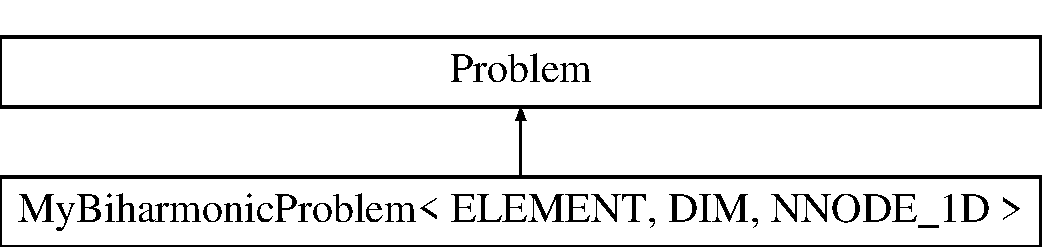
\includegraphics[height=2.000000cm]{classMyBiharmonicProblem}
\end{center}
\end{figure}
\subsection*{Public Member Functions}
\begin{DoxyCompactItemize}
\item 
\hyperlink{classMyBiharmonicProblem_ab894abf54210a71c3b4e00e1b30e380e}{My\+Biharmonic\+Problem} (typename \hyperlink{classoomph_1_1MyBiharmonicEquations}{My\+Biharmonic\+Equations}$<$ D\+IM, N\+N\+O\+D\+E\+\_\+1D $>$\+::Source\+Fct\+Pt source\+\_\+fct\+\_\+pt, typename \hyperlink{classoomph_1_1MyBiharmonicEquations}{My\+Biharmonic\+Equations}$<$ D\+IM, N\+N\+O\+D\+E\+\_\+1D $>$\+::Exact\+Soln\+Pt exact\+\_\+pt, const string \&node\+\_\+file\+\_\+name, const string \&element\+\_\+file\+\_\+name, const string \&poly\+\_\+file\+\_\+name)
\begin{DoxyCompactList}\small\item\em Constructor\+: Pass number of elements and pointer to source function. \end{DoxyCompactList}\item 
\hyperlink{classMyBiharmonicProblem_ad6d1bdce803ec5fd13bf6b0e3b1f3ca9}{$\sim$\+My\+Biharmonic\+Problem} ()
\begin{DoxyCompactList}\small\item\em Destructor (empty) \end{DoxyCompactList}\item 
void \hyperlink{classMyBiharmonicProblem_ae9a9d6db2c84c3cc12138558b60d676d}{actions\+\_\+before\+\_\+newton\+\_\+solve} ()
\begin{DoxyCompactList}\small\item\em Update the problem specs before solve\+: (Re)set boundary conditions. \end{DoxyCompactList}\item 
void \hyperlink{classMyBiharmonicProblem_a0600c4a7dff6f362b6171c66e07b594c}{actions\+\_\+after\+\_\+newton\+\_\+solve} ()
\begin{DoxyCompactList}\small\item\em Update the problem specs after solve (empty) \end{DoxyCompactList}\item 
void \hyperlink{classMyBiharmonicProblem_aa1c9d6b8298b2b78f5df9343349ecd70}{doc\+\_\+solution} (Doc\+Info \&doc\+\_\+info)
\begin{DoxyCompactList}\small\item\em Doc the solution, pass the number of the case considered, so that output files can be distinguished. \end{DoxyCompactList}\item 
void \hyperlink{classMyBiharmonicProblem_a40167119fb35b4926185b7adc23a6358}{nodal\+\_\+permutation} ()
\begin{DoxyCompactList}\small\item\em Perform a nodal permutation in curved elements. \end{DoxyCompactList}\end{DoxyCompactItemize}
\subsection*{Private Attributes}
\begin{DoxyCompactItemize}
\item 
\hyperlink{classoomph_1_1MyBiharmonicEquations}{My\+Biharmonic\+Equations}$<$ D\+IM, N\+N\+O\+D\+E\+\_\+1D $>$\+::Source\+Fct\+Pt \hyperlink{classMyBiharmonicProblem_a1ba6c64955d32e319db7a7de7807458a}{Source\+\_\+fct\+\_\+pt}
\begin{DoxyCompactList}\small\item\em Pointer to source function. \end{DoxyCompactList}\item 
\hyperlink{classoomph_1_1MyBiharmonicEquations}{My\+Biharmonic\+Equations}$<$ D\+IM, N\+N\+O\+D\+E\+\_\+1D $>$\+::Exact\+Soln\+Pt \hyperlink{classMyBiharmonicProblem_a9f681412ab2041bf3ddcd668ee816362}{Exact\+\_\+soln\+\_\+pt}
\begin{DoxyCompactList}\small\item\em Pointer to the exact solution. \end{DoxyCompactList}\end{DoxyCompactItemize}


\subsection{Detailed Description}
\subsubsection*{template$<$class E\+L\+E\+M\+E\+NT, unsigned D\+IM, unsigned N\+N\+O\+D\+E\+\_\+1D$>$\newline
class My\+Biharmonic\+Problem$<$ E\+L\+E\+M\+E\+N\+T, D\+I\+M, N\+N\+O\+D\+E\+\_\+1\+D $>$}

2D Biharmonic problem. 

Definition at line 1174 of file unstructured\+\_\+2d\+\_\+biharmonic\+\_\+curvedelement.\+cc.



\subsection{Constructor \& Destructor Documentation}
\mbox{\Hypertarget{classMyBiharmonicProblem_ab894abf54210a71c3b4e00e1b30e380e}\label{classMyBiharmonicProblem_ab894abf54210a71c3b4e00e1b30e380e}} 
\index{My\+Biharmonic\+Problem@{My\+Biharmonic\+Problem}!My\+Biharmonic\+Problem@{My\+Biharmonic\+Problem}}
\index{My\+Biharmonic\+Problem@{My\+Biharmonic\+Problem}!My\+Biharmonic\+Problem@{My\+Biharmonic\+Problem}}
\subsubsection{\texorpdfstring{My\+Biharmonic\+Problem()}{MyBiharmonicProblem()}}
{\footnotesize\ttfamily template$<$class E\+L\+E\+M\+E\+NT , unsigned D\+IM, unsigned N\+N\+O\+D\+E\+\_\+1D$>$ \\
\hyperlink{classMyBiharmonicProblem}{My\+Biharmonic\+Problem}$<$ E\+L\+E\+M\+E\+NT, D\+IM, N\+N\+O\+D\+E\+\_\+1D $>$\+::\hyperlink{classMyBiharmonicProblem}{My\+Biharmonic\+Problem} (\begin{DoxyParamCaption}\item[{typename \hyperlink{classoomph_1_1MyBiharmonicEquations}{My\+Biharmonic\+Equations}$<$ D\+IM, N\+N\+O\+D\+E\+\_\+1D $>$\+::Source\+Fct\+Pt}]{source\+\_\+fct\+\_\+pt,  }\item[{typename \hyperlink{classoomph_1_1MyBiharmonicEquations}{My\+Biharmonic\+Equations}$<$ D\+IM, N\+N\+O\+D\+E\+\_\+1D $>$\+::Exact\+Soln\+Pt}]{exact\+\_\+pt,  }\item[{const string \&}]{node\+\_\+file\+\_\+name,  }\item[{const string \&}]{element\+\_\+file\+\_\+name,  }\item[{const string \&}]{poly\+\_\+file\+\_\+name }\end{DoxyParamCaption})}



Constructor\+: Pass number of elements and pointer to source function. 

Constructor for 2D Biharmonic problem. Discretise the 2D domain with n\+\_\+element elements of type E\+L\+E\+M\+E\+NT. Specify function pointer to source function. 

Definition at line 1226 of file unstructured\+\_\+2d\+\_\+biharmonic\+\_\+curvedelement.\+cc.

\mbox{\Hypertarget{classMyBiharmonicProblem_ad6d1bdce803ec5fd13bf6b0e3b1f3ca9}\label{classMyBiharmonicProblem_ad6d1bdce803ec5fd13bf6b0e3b1f3ca9}} 
\index{My\+Biharmonic\+Problem@{My\+Biharmonic\+Problem}!````~My\+Biharmonic\+Problem@{$\sim$\+My\+Biharmonic\+Problem}}
\index{````~My\+Biharmonic\+Problem@{$\sim$\+My\+Biharmonic\+Problem}!My\+Biharmonic\+Problem@{My\+Biharmonic\+Problem}}
\subsubsection{\texorpdfstring{$\sim$\+My\+Biharmonic\+Problem()}{~MyBiharmonicProblem()}}
{\footnotesize\ttfamily template$<$class E\+L\+E\+M\+E\+NT, unsigned D\+IM, unsigned N\+N\+O\+D\+E\+\_\+1D$>$ \\
\hyperlink{classMyBiharmonicProblem}{My\+Biharmonic\+Problem}$<$ E\+L\+E\+M\+E\+NT, D\+IM, N\+N\+O\+D\+E\+\_\+1D $>$\+::$\sim$\hyperlink{classMyBiharmonicProblem}{My\+Biharmonic\+Problem} (\begin{DoxyParamCaption}{ }\end{DoxyParamCaption})\hspace{0.3cm}{\ttfamily [inline]}}



Destructor (empty) 



Definition at line 1186 of file unstructured\+\_\+2d\+\_\+biharmonic\+\_\+curvedelement.\+cc.



\subsection{Member Function Documentation}
\mbox{\Hypertarget{classMyBiharmonicProblem_a0600c4a7dff6f362b6171c66e07b594c}\label{classMyBiharmonicProblem_a0600c4a7dff6f362b6171c66e07b594c}} 
\index{My\+Biharmonic\+Problem@{My\+Biharmonic\+Problem}!actions\+\_\+after\+\_\+newton\+\_\+solve@{actions\+\_\+after\+\_\+newton\+\_\+solve}}
\index{actions\+\_\+after\+\_\+newton\+\_\+solve@{actions\+\_\+after\+\_\+newton\+\_\+solve}!My\+Biharmonic\+Problem@{My\+Biharmonic\+Problem}}
\subsubsection{\texorpdfstring{actions\+\_\+after\+\_\+newton\+\_\+solve()}{actions\_after\_newton\_solve()}}
{\footnotesize\ttfamily template$<$class E\+L\+E\+M\+E\+NT, unsigned D\+IM, unsigned N\+N\+O\+D\+E\+\_\+1D$>$ \\
void \hyperlink{classMyBiharmonicProblem}{My\+Biharmonic\+Problem}$<$ E\+L\+E\+M\+E\+NT, D\+IM, N\+N\+O\+D\+E\+\_\+1D $>$\+::actions\+\_\+after\+\_\+newton\+\_\+solve (\begin{DoxyParamCaption}{ }\end{DoxyParamCaption})\hspace{0.3cm}{\ttfamily [inline]}}



Update the problem specs after solve (empty) 



Definition at line 1196 of file unstructured\+\_\+2d\+\_\+biharmonic\+\_\+curvedelement.\+cc.

\mbox{\Hypertarget{classMyBiharmonicProblem_ae9a9d6db2c84c3cc12138558b60d676d}\label{classMyBiharmonicProblem_ae9a9d6db2c84c3cc12138558b60d676d}} 
\index{My\+Biharmonic\+Problem@{My\+Biharmonic\+Problem}!actions\+\_\+before\+\_\+newton\+\_\+solve@{actions\+\_\+before\+\_\+newton\+\_\+solve}}
\index{actions\+\_\+before\+\_\+newton\+\_\+solve@{actions\+\_\+before\+\_\+newton\+\_\+solve}!My\+Biharmonic\+Problem@{My\+Biharmonic\+Problem}}
\subsubsection{\texorpdfstring{actions\+\_\+before\+\_\+newton\+\_\+solve()}{actions\_before\_newton\_solve()}}
{\footnotesize\ttfamily template$<$class E\+L\+E\+M\+E\+NT , unsigned D\+IM, unsigned N\+N\+O\+D\+E\+\_\+1D$>$ \\
void \hyperlink{classMyBiharmonicProblem}{My\+Biharmonic\+Problem}$<$ E\+L\+E\+M\+E\+NT, D\+IM, N\+N\+O\+D\+E\+\_\+1D $>$\+::actions\+\_\+before\+\_\+newton\+\_\+solve (\begin{DoxyParamCaption}{ }\end{DoxyParamCaption})}



Update the problem specs before solve\+: (Re)set boundary conditions. 

Update the problem specs before solve\+: (Re)set boundary values from the exact solution. 

Definition at line 1502 of file unstructured\+\_\+2d\+\_\+biharmonic\+\_\+curvedelement.\+cc.



References Physical\+\_\+\+Variables\+::get\+\_\+exact\+\_\+u().

\mbox{\Hypertarget{classMyBiharmonicProblem_aa1c9d6b8298b2b78f5df9343349ecd70}\label{classMyBiharmonicProblem_aa1c9d6b8298b2b78f5df9343349ecd70}} 
\index{My\+Biharmonic\+Problem@{My\+Biharmonic\+Problem}!doc\+\_\+solution@{doc\+\_\+solution}}
\index{doc\+\_\+solution@{doc\+\_\+solution}!My\+Biharmonic\+Problem@{My\+Biharmonic\+Problem}}
\subsubsection{\texorpdfstring{doc\+\_\+solution()}{doc\_solution()}}
{\footnotesize\ttfamily template$<$class E\+L\+E\+M\+E\+NT , unsigned D\+IM, unsigned N\+N\+O\+D\+E\+\_\+1D$>$ \\
void \hyperlink{classMyBiharmonicProblem}{My\+Biharmonic\+Problem}$<$ E\+L\+E\+M\+E\+NT, D\+IM, N\+N\+O\+D\+E\+\_\+1D $>$\+::doc\+\_\+solution (\begin{DoxyParamCaption}\item[{Doc\+Info \&}]{doc\+\_\+info }\end{DoxyParamCaption})}



Doc the solution, pass the number of the case considered, so that output files can be distinguished. 

Doc the solution in tecplot format. Label files with label. 

Definition at line 1542 of file unstructured\+\_\+2d\+\_\+biharmonic\+\_\+curvedelement.\+cc.



References Physical\+\_\+\+Variables\+::get\+\_\+exact\+\_\+u().



Referenced by main().

\mbox{\Hypertarget{classMyBiharmonicProblem_a40167119fb35b4926185b7adc23a6358}\label{classMyBiharmonicProblem_a40167119fb35b4926185b7adc23a6358}} 
\index{My\+Biharmonic\+Problem@{My\+Biharmonic\+Problem}!nodal\+\_\+permutation@{nodal\+\_\+permutation}}
\index{nodal\+\_\+permutation@{nodal\+\_\+permutation}!My\+Biharmonic\+Problem@{My\+Biharmonic\+Problem}}
\subsubsection{\texorpdfstring{nodal\+\_\+permutation()}{nodal\_permutation()}}
{\footnotesize\ttfamily template$<$class E\+L\+E\+M\+E\+NT , unsigned D\+IM, unsigned N\+N\+O\+D\+E\+\_\+1D$>$ \\
void \hyperlink{classMyBiharmonicProblem}{My\+Biharmonic\+Problem}$<$ E\+L\+E\+M\+E\+NT, D\+IM, N\+N\+O\+D\+E\+\_\+1D $>$\+::nodal\+\_\+permutation (\begin{DoxyParamCaption}{ }\end{DoxyParamCaption})}



Perform a nodal permutation in curved elements. 

Update the nodal permutation in curved elements\+: (Re)assign coordinates so that the first and the second nodes are associated with the lower and upper position on a boundary, respectively. The third node is off-\/boundary node. Permutation just for the curved elements 

Definition at line 1359 of file unstructured\+\_\+2d\+\_\+biharmonic\+\_\+curvedelement.\+cc.



\subsection{Member Data Documentation}
\mbox{\Hypertarget{classMyBiharmonicProblem_a9f681412ab2041bf3ddcd668ee816362}\label{classMyBiharmonicProblem_a9f681412ab2041bf3ddcd668ee816362}} 
\index{My\+Biharmonic\+Problem@{My\+Biharmonic\+Problem}!Exact\+\_\+soln\+\_\+pt@{Exact\+\_\+soln\+\_\+pt}}
\index{Exact\+\_\+soln\+\_\+pt@{Exact\+\_\+soln\+\_\+pt}!My\+Biharmonic\+Problem@{My\+Biharmonic\+Problem}}
\subsubsection{\texorpdfstring{Exact\+\_\+soln\+\_\+pt}{Exact\_soln\_pt}}
{\footnotesize\ttfamily template$<$class E\+L\+E\+M\+E\+NT, unsigned D\+IM, unsigned N\+N\+O\+D\+E\+\_\+1D$>$ \\
\hyperlink{classoomph_1_1MyBiharmonicEquations}{My\+Biharmonic\+Equations}$<$D\+IM,N\+N\+O\+D\+E\+\_\+1D$>$\+::Exact\+Soln\+Pt \hyperlink{classMyBiharmonicProblem}{My\+Biharmonic\+Problem}$<$ E\+L\+E\+M\+E\+NT, D\+IM, N\+N\+O\+D\+E\+\_\+1D $>$\+::Exact\+\_\+soln\+\_\+pt\hspace{0.3cm}{\ttfamily [private]}}



Pointer to the exact solution. 



Definition at line 1211 of file unstructured\+\_\+2d\+\_\+biharmonic\+\_\+curvedelement.\+cc.

\mbox{\Hypertarget{classMyBiharmonicProblem_a1ba6c64955d32e319db7a7de7807458a}\label{classMyBiharmonicProblem_a1ba6c64955d32e319db7a7de7807458a}} 
\index{My\+Biharmonic\+Problem@{My\+Biharmonic\+Problem}!Source\+\_\+fct\+\_\+pt@{Source\+\_\+fct\+\_\+pt}}
\index{Source\+\_\+fct\+\_\+pt@{Source\+\_\+fct\+\_\+pt}!My\+Biharmonic\+Problem@{My\+Biharmonic\+Problem}}
\subsubsection{\texorpdfstring{Source\+\_\+fct\+\_\+pt}{Source\_fct\_pt}}
{\footnotesize\ttfamily template$<$class E\+L\+E\+M\+E\+NT, unsigned D\+IM, unsigned N\+N\+O\+D\+E\+\_\+1D$>$ \\
\hyperlink{classoomph_1_1MyBiharmonicEquations}{My\+Biharmonic\+Equations}$<$D\+IM,N\+N\+O\+D\+E\+\_\+1D$>$\+::Source\+Fct\+Pt \hyperlink{classMyBiharmonicProblem}{My\+Biharmonic\+Problem}$<$ E\+L\+E\+M\+E\+NT, D\+IM, N\+N\+O\+D\+E\+\_\+1D $>$\+::Source\+\_\+fct\+\_\+pt\hspace{0.3cm}{\ttfamily [private]}}



Pointer to source function. 



Definition at line 1208 of file unstructured\+\_\+2d\+\_\+biharmonic\+\_\+curvedelement.\+cc.



The documentation for this class was generated from the following file\+:\begin{DoxyCompactItemize}
\item 
\hyperlink{unstructured__2d__biharmonic__curvedelement_8cc}{unstructured\+\_\+2d\+\_\+biharmonic\+\_\+curvedelement.\+cc}\end{DoxyCompactItemize}

\chapter{File Documentation}
\hypertarget{curved__element_8txt__doxygenified_8h}{}\section{curved\+\_\+element.\+txt\+\_\+doxygenified.\+h File Reference}
\label{curved__element_8txt__doxygenified_8h}\index{curved\+\_\+element.\+txt\+\_\+doxygenified.\+h@{curved\+\_\+element.\+txt\+\_\+doxygenified.\+h}}

\hypertarget{unstructured__2d__biharmonic__bellelement_8cc}{}\section{unstructured\+\_\+2d\+\_\+biharmonic\+\_\+bellelement.\+cc File Reference}
\label{unstructured__2d__biharmonic__bellelement_8cc}\index{unstructured\+\_\+2d\+\_\+biharmonic\+\_\+bellelement.\+cc@{unstructured\+\_\+2d\+\_\+biharmonic\+\_\+bellelement.\+cc}}
{\ttfamily \#include \char`\"{}generic.\+h\char`\"{}}\newline
{\ttfamily \#include \char`\"{}meshes/one\+\_\+d\+\_\+mesh.\+h\char`\"{}}\newline
{\ttfamily \#include \char`\"{}meshes/simple\+\_\+rectangular\+\_\+tri\+\_\+mesh.\+h\char`\"{}}\newline
{\ttfamily \#include \char`\"{}meshes/simple\+\_\+rectangular\+\_\+quadmesh.\+h\char`\"{}}\newline
{\ttfamily \#include \char`\"{}generic/geom\+\_\+objects.\+h\char`\"{}}\newline
{\ttfamily \#include \char`\"{}meshes/triangle\+\_\+mesh.\+h\char`\"{}}\newline
\subsection*{Classes}
\begin{DoxyCompactItemize}
\item 
class \hyperlink{classoomph_1_1MyBiharmonicEquations}{oomph\+::\+My\+Biharmonic\+Equations$<$ D\+I\+M, N\+N\+O\+D\+E\+\_\+1\+D $>$}
\item 
class \hyperlink{classoomph_1_1BellBiharmonicElement}{oomph\+::\+Bell\+Biharmonic\+Element$<$ D\+I\+M, N\+N\+O\+D\+E\+\_\+1\+D $>$}
\item 
class \hyperlink{classoomph_1_1FaceGeometry_3_01BellBiharmonicElement_3_01DIM_00_01NNODE__1D_01_4_01_4}{oomph\+::\+Face\+Geometry$<$ Bell\+Biharmonic\+Element$<$ D\+I\+M, N\+N\+O\+D\+E\+\_\+1\+D $>$ $>$}
\item 
class \hyperlink{classBiharmonicProblem}{Biharmonic\+Problem$<$ E\+L\+E\+M\+E\+N\+T, D\+I\+M, N\+N\+O\+D\+E\+\_\+1\+D $>$}
\begin{DoxyCompactList}\small\item\em 2D Biharmonic problem. \end{DoxyCompactList}\end{DoxyCompactItemize}
\subsection*{Namespaces}
\begin{DoxyCompactItemize}
\item 
 \hyperlink{namespaceoomph}{oomph}
\item 
 \hyperlink{namespacePhysical__Variables}{Physical\+\_\+\+Variables}
\begin{DoxyCompactList}\small\item\em Namespace for the solution of 2D Biharmonic equation. \end{DoxyCompactList}\end{DoxyCompactItemize}
\subsection*{Macros}
\begin{DoxyCompactItemize}
\item 
\#define \hyperlink{unstructured__2d__biharmonic__bellelement_8cc_a13287952f5fdf4c8f41200a50b0afc38}{O\+O\+M\+P\+H\+\_\+\+B\+I\+H\+A\+R\+M\+O\+N\+I\+C\+\_\+\+B\+E\+L\+L\+\_\+\+E\+L\+E\+M\+E\+N\+T\+S\+\_\+\+H\+E\+A\+D\+ER}
\end{DoxyCompactItemize}
\subsection*{Functions}
\begin{DoxyCompactItemize}
\item 
void \hyperlink{namespacePhysical__Variables_af90d0c580c57b1152fd1cc7046055031}{Physical\+\_\+\+Variables\+::get\+\_\+exact\+\_\+u} (const Vector$<$ double $>$ \&x, Vector$<$ double $>$ \&u)
\begin{DoxyCompactList}\small\item\em Exact solution as a Vector. \end{DoxyCompactList}\item 
void \hyperlink{namespacePhysical__Variables_ae11027d76c5f512b7db6a1b6d17dc792}{Physical\+\_\+\+Variables\+::source\+\_\+function} (const Vector$<$ double $>$ \&x, double \&source)
\begin{DoxyCompactList}\small\item\em Source function required to make the above exact solution. \end{DoxyCompactList}\item 
int \hyperlink{unstructured__2d__biharmonic__bellelement_8cc_a0ddf1224851353fc92bfbff6f499fa97}{main} (int argc, char $\ast$argv\mbox{[}$\,$\mbox{]})
\begin{DoxyCompactList}\small\item\em Driver for the Biharmonic equation. \end{DoxyCompactList}\end{DoxyCompactItemize}


\subsection{Macro Definition Documentation}
\mbox{\Hypertarget{unstructured__2d__biharmonic__bellelement_8cc_a13287952f5fdf4c8f41200a50b0afc38}\label{unstructured__2d__biharmonic__bellelement_8cc_a13287952f5fdf4c8f41200a50b0afc38}} 
\index{unstructured\+\_\+2d\+\_\+biharmonic\+\_\+bellelement.\+cc@{unstructured\+\_\+2d\+\_\+biharmonic\+\_\+bellelement.\+cc}!O\+O\+M\+P\+H\+\_\+\+B\+I\+H\+A\+R\+M\+O\+N\+I\+C\+\_\+\+B\+E\+L\+L\+\_\+\+E\+L\+E\+M\+E\+N\+T\+S\+\_\+\+H\+E\+A\+D\+ER@{O\+O\+M\+P\+H\+\_\+\+B\+I\+H\+A\+R\+M\+O\+N\+I\+C\+\_\+\+B\+E\+L\+L\+\_\+\+E\+L\+E\+M\+E\+N\+T\+S\+\_\+\+H\+E\+A\+D\+ER}}
\index{O\+O\+M\+P\+H\+\_\+\+B\+I\+H\+A\+R\+M\+O\+N\+I\+C\+\_\+\+B\+E\+L\+L\+\_\+\+E\+L\+E\+M\+E\+N\+T\+S\+\_\+\+H\+E\+A\+D\+ER@{O\+O\+M\+P\+H\+\_\+\+B\+I\+H\+A\+R\+M\+O\+N\+I\+C\+\_\+\+B\+E\+L\+L\+\_\+\+E\+L\+E\+M\+E\+N\+T\+S\+\_\+\+H\+E\+A\+D\+ER}!unstructured\+\_\+2d\+\_\+biharmonic\+\_\+bellelement.\+cc@{unstructured\+\_\+2d\+\_\+biharmonic\+\_\+bellelement.\+cc}}
\subsubsection{\texorpdfstring{O\+O\+M\+P\+H\+\_\+\+B\+I\+H\+A\+R\+M\+O\+N\+I\+C\+\_\+\+B\+E\+L\+L\+\_\+\+E\+L\+E\+M\+E\+N\+T\+S\+\_\+\+H\+E\+A\+D\+ER}{OOMPH\_BIHARMONIC\_BELL\_ELEMENTS\_HEADER}}
{\footnotesize\ttfamily \#define O\+O\+M\+P\+H\+\_\+\+B\+I\+H\+A\+R\+M\+O\+N\+I\+C\+\_\+\+B\+E\+L\+L\+\_\+\+E\+L\+E\+M\+E\+N\+T\+S\+\_\+\+H\+E\+A\+D\+ER}



Definition at line 54 of file unstructured\+\_\+2d\+\_\+biharmonic\+\_\+bellelement.\+cc.



\subsection{Function Documentation}
\mbox{\Hypertarget{unstructured__2d__biharmonic__bellelement_8cc_a0ddf1224851353fc92bfbff6f499fa97}\label{unstructured__2d__biharmonic__bellelement_8cc_a0ddf1224851353fc92bfbff6f499fa97}} 
\index{unstructured\+\_\+2d\+\_\+biharmonic\+\_\+bellelement.\+cc@{unstructured\+\_\+2d\+\_\+biharmonic\+\_\+bellelement.\+cc}!main@{main}}
\index{main@{main}!unstructured\+\_\+2d\+\_\+biharmonic\+\_\+bellelement.\+cc@{unstructured\+\_\+2d\+\_\+biharmonic\+\_\+bellelement.\+cc}}
\subsubsection{\texorpdfstring{main()}{main()}}
{\footnotesize\ttfamily int main (\begin{DoxyParamCaption}\item[{int}]{argc,  }\item[{char $\ast$}]{argv\mbox{[}$\,$\mbox{]} }\end{DoxyParamCaption})}



Driver for the Biharmonic equation. 



Definition at line 1162 of file unstructured\+\_\+2d\+\_\+biharmonic\+\_\+bellelement.\+cc.



References Biharmonic\+Problem$<$ E\+L\+E\+M\+E\+N\+T, D\+I\+M, N\+N\+O\+D\+E\+\_\+1\+D $>$\+::doc\+\_\+solution(), and Physical\+\_\+\+Variables\+::source\+\_\+function().


\hypertarget{unstructured__2d__biharmonic__curvedelement_8cc}{}\section{unstructured\+\_\+2d\+\_\+biharmonic\+\_\+curvedelement.\+cc File Reference}
\label{unstructured__2d__biharmonic__curvedelement_8cc}\index{unstructured\+\_\+2d\+\_\+biharmonic\+\_\+curvedelement.\+cc@{unstructured\+\_\+2d\+\_\+biharmonic\+\_\+curvedelement.\+cc}}
{\ttfamily \#include \char`\"{}generic.\+h\char`\"{}}\newline
{\ttfamily \#include \char`\"{}meshes/one\+\_\+d\+\_\+mesh.\+h\char`\"{}}\newline
{\ttfamily \#include \char`\"{}meshes/simple\+\_\+rectangular\+\_\+tri\+\_\+mesh.\+h\char`\"{}}\newline
{\ttfamily \#include \char`\"{}meshes/simple\+\_\+rectangular\+\_\+quadmesh.\+h\char`\"{}}\newline
{\ttfamily \#include \char`\"{}generic/geom\+\_\+objects.\+h\char`\"{}}\newline
{\ttfamily \#include \char`\"{}meshes/triangle\+\_\+mesh.\+h\char`\"{}}\newline
\subsection*{Classes}
\begin{DoxyCompactItemize}
\item 
class \hyperlink{classoomph_1_1MyBiharmonicEquations}{oomph\+::\+My\+Biharmonic\+Equations$<$ D\+I\+M, N\+N\+O\+D\+E\+\_\+1\+D $>$}
\item 
class \hyperlink{classoomph_1_1BiharmonicCurvedElement}{oomph\+::\+Biharmonic\+Curved\+Element$<$ D\+I\+M, N\+N\+O\+D\+E\+\_\+1\+D $>$}
\item 
class \hyperlink{classoomph_1_1FaceGeometry_3_01BiharmonicCurvedElement_3_01DIM_00_01NNODE__1D_01_4_01_4}{oomph\+::\+Face\+Geometry$<$ Biharmonic\+Curved\+Element$<$ D\+I\+M, N\+N\+O\+D\+E\+\_\+1\+D $>$ $>$}
\item 
class \hyperlink{classMyBiharmonicProblem}{My\+Biharmonic\+Problem$<$ E\+L\+E\+M\+E\+N\+T, D\+I\+M, N\+N\+O\+D\+E\+\_\+1\+D $>$}
\begin{DoxyCompactList}\small\item\em 2D Biharmonic problem. \end{DoxyCompactList}\end{DoxyCompactItemize}
\subsection*{Namespaces}
\begin{DoxyCompactItemize}
\item 
 \hyperlink{namespaceoomph}{oomph}
\item 
 \hyperlink{namespacePhysical__Variables}{Physical\+\_\+\+Variables}
\begin{DoxyCompactList}\small\item\em Namespace for the solution of 2D Biharmonic equation. \end{DoxyCompactList}\end{DoxyCompactItemize}
\subsection*{Macros}
\begin{DoxyCompactItemize}
\item 
\#define \hyperlink{unstructured__2d__biharmonic__curvedelement_8cc_a755d68c72863c25f9c46090d29e8be89}{O\+O\+M\+P\+H\+\_\+\+B\+I\+H\+A\+R\+M\+O\+N\+I\+C\+\_\+\+C\+U\+R\+V\+E\+D\+\_\+\+E\+L\+E\+M\+E\+N\+T\+S\+\_\+\+H\+E\+A\+D\+ER}
\end{DoxyCompactItemize}
\subsection*{Functions}
\begin{DoxyCompactItemize}
\item 
void \hyperlink{namespacePhysical__Variables_af90d0c580c57b1152fd1cc7046055031}{Physical\+\_\+\+Variables\+::get\+\_\+exact\+\_\+u} (const Vector$<$ double $>$ \&x, Vector$<$ double $>$ \&u)
\begin{DoxyCompactList}\small\item\em Exact solution as a Vector. \end{DoxyCompactList}\item 
void \hyperlink{namespacePhysical__Variables_ae11027d76c5f512b7db6a1b6d17dc792}{Physical\+\_\+\+Variables\+::source\+\_\+function} (const Vector$<$ double $>$ \&x, double \&source)
\begin{DoxyCompactList}\small\item\em Source function required to make the above exact solution. \end{DoxyCompactList}\item 
int \hyperlink{unstructured__2d__biharmonic__curvedelement_8cc_a0ddf1224851353fc92bfbff6f499fa97}{main} (int argc, char $\ast$argv\mbox{[}$\,$\mbox{]})
\begin{DoxyCompactList}\small\item\em Driver for 2D Biharmonic problem. \end{DoxyCompactList}\end{DoxyCompactItemize}


\subsection{Macro Definition Documentation}
\mbox{\Hypertarget{unstructured__2d__biharmonic__curvedelement_8cc_a755d68c72863c25f9c46090d29e8be89}\label{unstructured__2d__biharmonic__curvedelement_8cc_a755d68c72863c25f9c46090d29e8be89}} 
\index{unstructured\+\_\+2d\+\_\+biharmonic\+\_\+curvedelement.\+cc@{unstructured\+\_\+2d\+\_\+biharmonic\+\_\+curvedelement.\+cc}!O\+O\+M\+P\+H\+\_\+\+B\+I\+H\+A\+R\+M\+O\+N\+I\+C\+\_\+\+C\+U\+R\+V\+E\+D\+\_\+\+E\+L\+E\+M\+E\+N\+T\+S\+\_\+\+H\+E\+A\+D\+ER@{O\+O\+M\+P\+H\+\_\+\+B\+I\+H\+A\+R\+M\+O\+N\+I\+C\+\_\+\+C\+U\+R\+V\+E\+D\+\_\+\+E\+L\+E\+M\+E\+N\+T\+S\+\_\+\+H\+E\+A\+D\+ER}}
\index{O\+O\+M\+P\+H\+\_\+\+B\+I\+H\+A\+R\+M\+O\+N\+I\+C\+\_\+\+C\+U\+R\+V\+E\+D\+\_\+\+E\+L\+E\+M\+E\+N\+T\+S\+\_\+\+H\+E\+A\+D\+ER@{O\+O\+M\+P\+H\+\_\+\+B\+I\+H\+A\+R\+M\+O\+N\+I\+C\+\_\+\+C\+U\+R\+V\+E\+D\+\_\+\+E\+L\+E\+M\+E\+N\+T\+S\+\_\+\+H\+E\+A\+D\+ER}!unstructured\+\_\+2d\+\_\+biharmonic\+\_\+curvedelement.\+cc@{unstructured\+\_\+2d\+\_\+biharmonic\+\_\+curvedelement.\+cc}}
\subsubsection{\texorpdfstring{O\+O\+M\+P\+H\+\_\+\+B\+I\+H\+A\+R\+M\+O\+N\+I\+C\+\_\+\+C\+U\+R\+V\+E\+D\+\_\+\+E\+L\+E\+M\+E\+N\+T\+S\+\_\+\+H\+E\+A\+D\+ER}{OOMPH\_BIHARMONIC\_CURVED\_ELEMENTS\_HEADER}}
{\footnotesize\ttfamily \#define O\+O\+M\+P\+H\+\_\+\+B\+I\+H\+A\+R\+M\+O\+N\+I\+C\+\_\+\+C\+U\+R\+V\+E\+D\+\_\+\+E\+L\+E\+M\+E\+N\+T\+S\+\_\+\+H\+E\+A\+D\+ER}



Definition at line 54 of file unstructured\+\_\+2d\+\_\+biharmonic\+\_\+curvedelement.\+cc.



\subsection{Function Documentation}
\mbox{\Hypertarget{unstructured__2d__biharmonic__curvedelement_8cc_a0ddf1224851353fc92bfbff6f499fa97}\label{unstructured__2d__biharmonic__curvedelement_8cc_a0ddf1224851353fc92bfbff6f499fa97}} 
\index{unstructured\+\_\+2d\+\_\+biharmonic\+\_\+curvedelement.\+cc@{unstructured\+\_\+2d\+\_\+biharmonic\+\_\+curvedelement.\+cc}!main@{main}}
\index{main@{main}!unstructured\+\_\+2d\+\_\+biharmonic\+\_\+curvedelement.\+cc@{unstructured\+\_\+2d\+\_\+biharmonic\+\_\+curvedelement.\+cc}}
\subsubsection{\texorpdfstring{main()}{main()}}
{\footnotesize\ttfamily int main (\begin{DoxyParamCaption}\item[{int}]{argc,  }\item[{char $\ast$}]{argv\mbox{[}$\,$\mbox{]} }\end{DoxyParamCaption})}



Driver for 2D Biharmonic problem. 



Definition at line 1591 of file unstructured\+\_\+2d\+\_\+biharmonic\+\_\+curvedelement.\+cc.



References My\+Biharmonic\+Problem$<$ E\+L\+E\+M\+E\+N\+T, D\+I\+M, N\+N\+O\+D\+E\+\_\+1\+D $>$\+::doc\+\_\+solution(), Physical\+\_\+\+Variables\+::get\+\_\+exact\+\_\+u(), and Physical\+\_\+\+Variables\+::source\+\_\+function().


%--- End generated contents ---

% Index
\backmatter
\newpage
\phantomsection
\clearemptydoublepage
\addcontentsline{toc}{chapter}{Index}
\printindex

\end{document}
